\documentclass[11pt,a4paper,dvipdfmx]{jsarticle}

%定数
\newcommand{\accessToken}{アクセストークン \index{あくせすとーくん@アクセストークン}}
\newcommand{\bj}{「BaconJam」\index{baconjam@BaconJam}}
\newcommand{\bracketref}[1]{(\ref{#1}) {\footnotesize (P.\pageref{#1})}}
\newcommand{\change}{\colorbox{orange}{\textcolor{white}{\textbf{変更}}}\xdotfill{1pt}[orange]}
\newcommand{\currentVersion}{\texttt{Ver1.2.3}}
\newcommand{\fix}{\colorbox{red}{\textcolor{white}{\textbf{修正}}}\xdotfill{1pt}[red]}
\newcommand{\imageref}[1]{図\ref{#1}}
\newcommand{\mi}{\texttt{Misskey} \index{misskey@Misskey}}
\newcommand{\new}{\colorbox{teal}{\textcolor{white}{\textbf{新規}}}\xdotfill{1pt}[teal]}
\newcommand{\nowplaying}{「なうぷれ投稿」 \index{なうぷれとうこう@なうぷれ投稿}}
\newcommand{\spotifydashboard}{\href{https://developer.spotify.com/dashboard}{Dashboard}}
\newcommand{\ttbox}[1]{\ovalbox{\texttt{#1}}}
\newcommand{\ver}[1]{\texttt{Ver#1}}
\newcommand{\clientId}{\texttt{ClientID} \index{clientid@ClientID}}
\newcommand{\clientSecret}{\texttt{ClientSecret} \index{clientsecret@ClientSecret}}

%目次に節まで表示
\setcounter{tocdepth}{3}

\usepackage[dvipdfm]{color}
\usepackage[dvipdfm]{graphicx}
\usepackage[dvipdfmx]{hyperref}
\usepackage{amsmath,amssymb}
\usepackage{amssymb}
\usepackage{ascmac}
\usepackage{bm}
\usepackage{caption}
\usepackage{colortbl}
\usepackage{fancybox}
\usepackage{ltablex}
\usepackage{makeidx}
\usepackage{okumacro}
\usepackage{pdfpages}
\usepackage{pxjahyper}
\usepackage{xhfill}

\hypersetup{% hyperrefオプションリスト
setpagesize=false,
 bookmarksnumbered=true,%
 bookmarksopen=true,%
 colorlinks=true,%
 linkcolor=blue,
 citecolor=red,
}

\makeindex

\title{\bj (\currentVersion) 操作説明書 }
\author{くろいぬ/Falhong-Cha}
\date{最終更新日:\today}

\begin{document}
\renewcommand{\labelenumi}{(\arabic{enumi})}

\begin{titlepage}
	\maketitle\thispagestyle{empty}
\end{titlepage}
\tableofcontents

\clearpage
\section{アプリの対応}
    \begin{enumerate}
        \item OS:android 5以上
    \end{enumerate}

\newpage
\section{\mi との連携}
\label{sec:misskey1}
    \subsection{\mi 側の設定}
    \label{sec:misskey2}
        \subsubsection{\accessToken の発行}
        \label{sec:misskey3}
            \begin{enumerate}
                \item \nowplaying したい\mi サーバーで二要素認証の設定が必要な場合は、\href{https://support.misskey.io/hc/ja/articles/9354169842191-%E4%BA%8C%E8%A6%81%E7%B4%A0%E8%AA%8D%E8%A8%BC%E3%81%AE%E8%A8%AD%E5%AE%9A%E3%81%AB%E3%81%A4%E3%81%84%E3%81%A6}{こちら}を参考にあらかじめ設定を行ってください。
                \label{item:misskey1}
                \item 設定画面の\ttbox{Misskey接続設定}を押下して、設定項目を展開してください。
                \label{item:misskey2}
                    \begin{figure}[htbp]
                        \begin{minipage}[b]{0.45\linewidth}
                            \centering
                            \fbox{
                                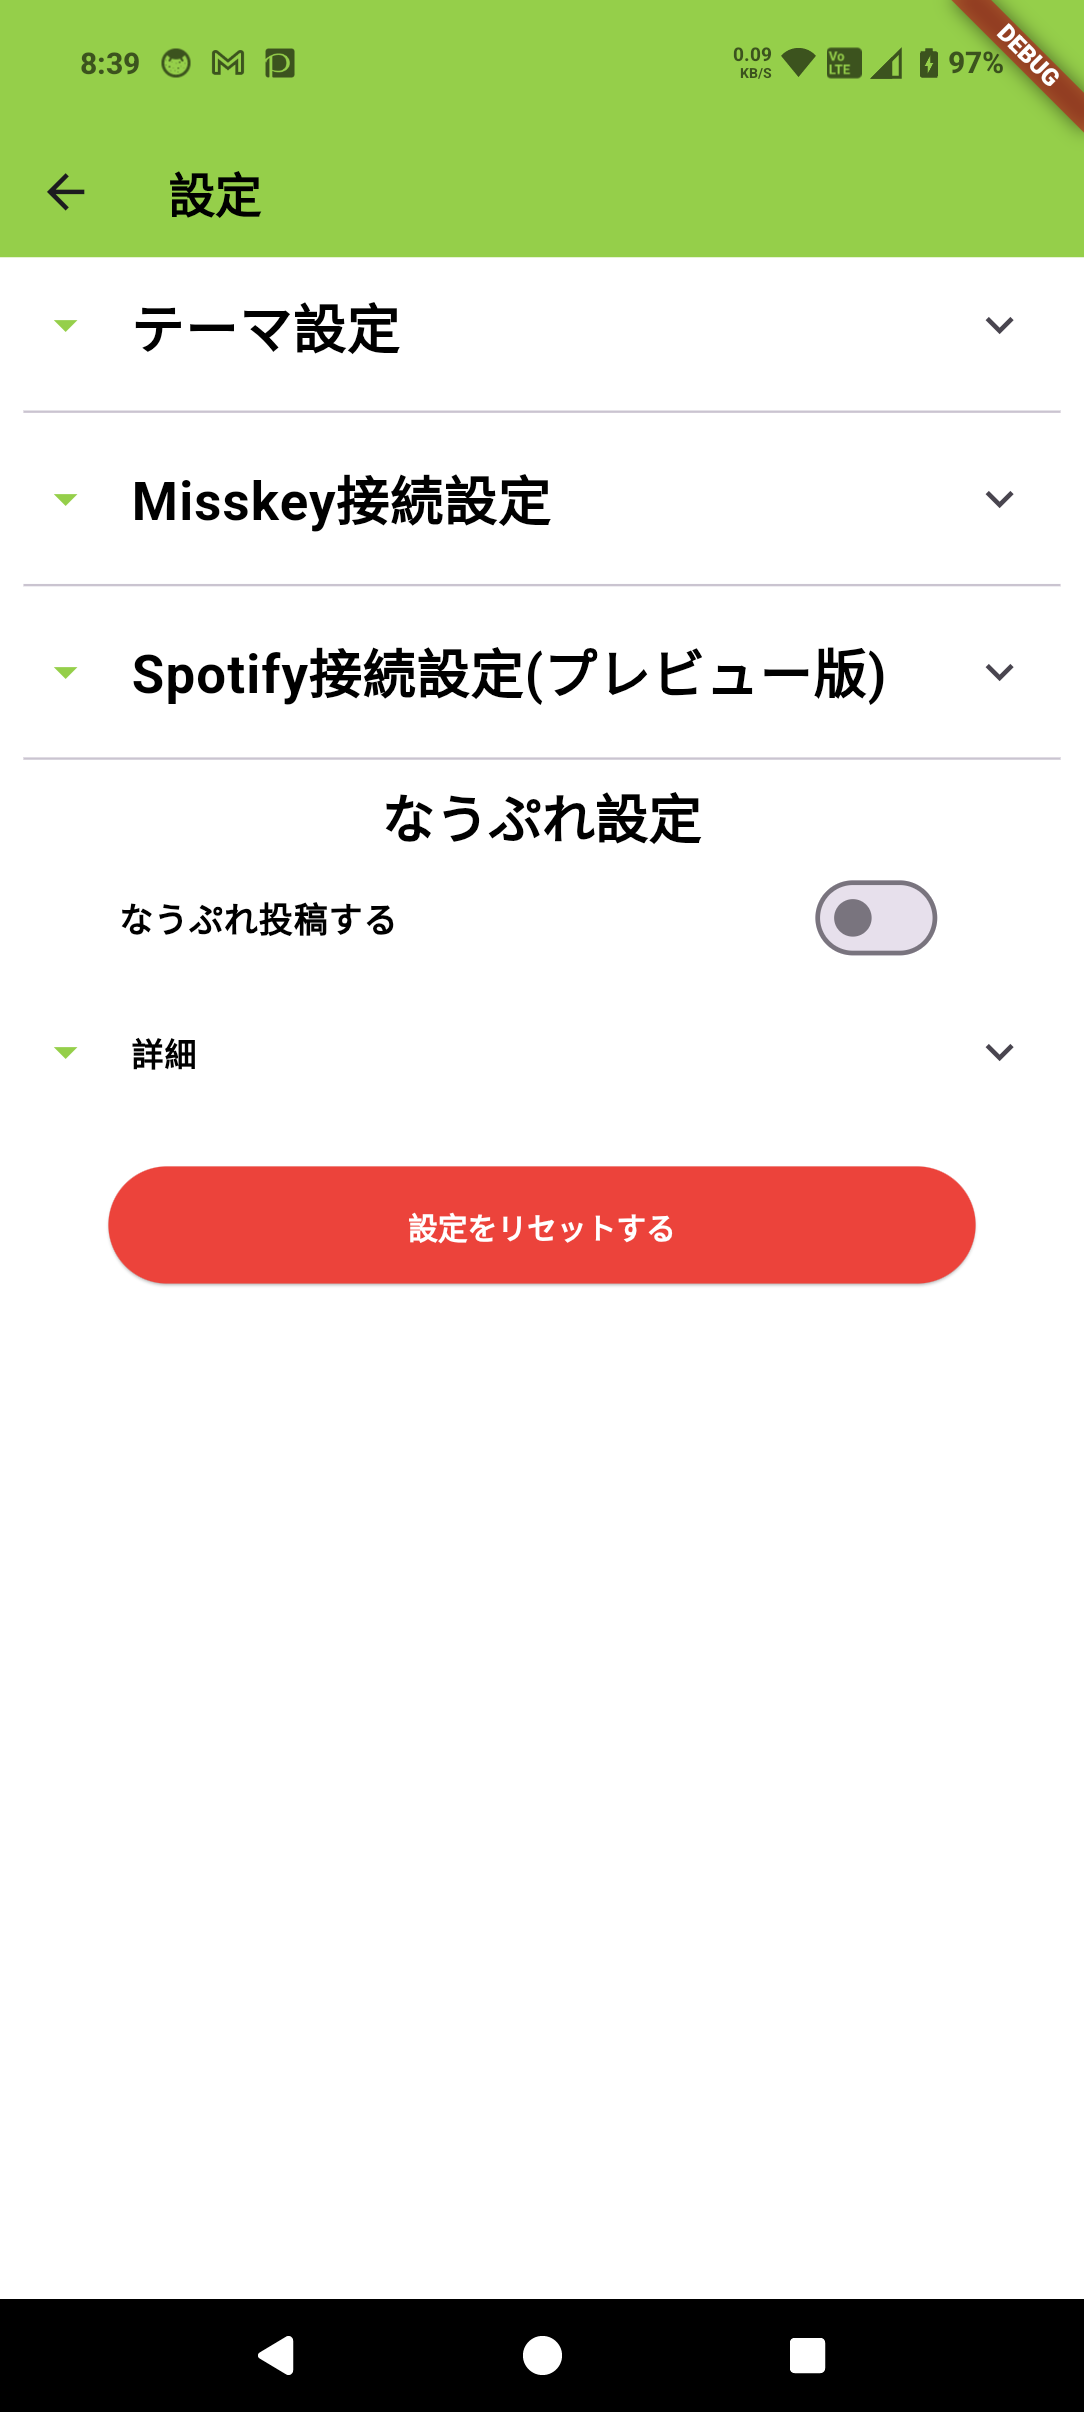
\includegraphics[width=5cm]{./pictures/misskey1.png}
                            }
                            \caption{展開前}
                            \label{img:misskey1}
                        \end{minipage}
                        \begin{minipage}[b]{0.45\linewidth}
                            \centering
                            \fbox{
                                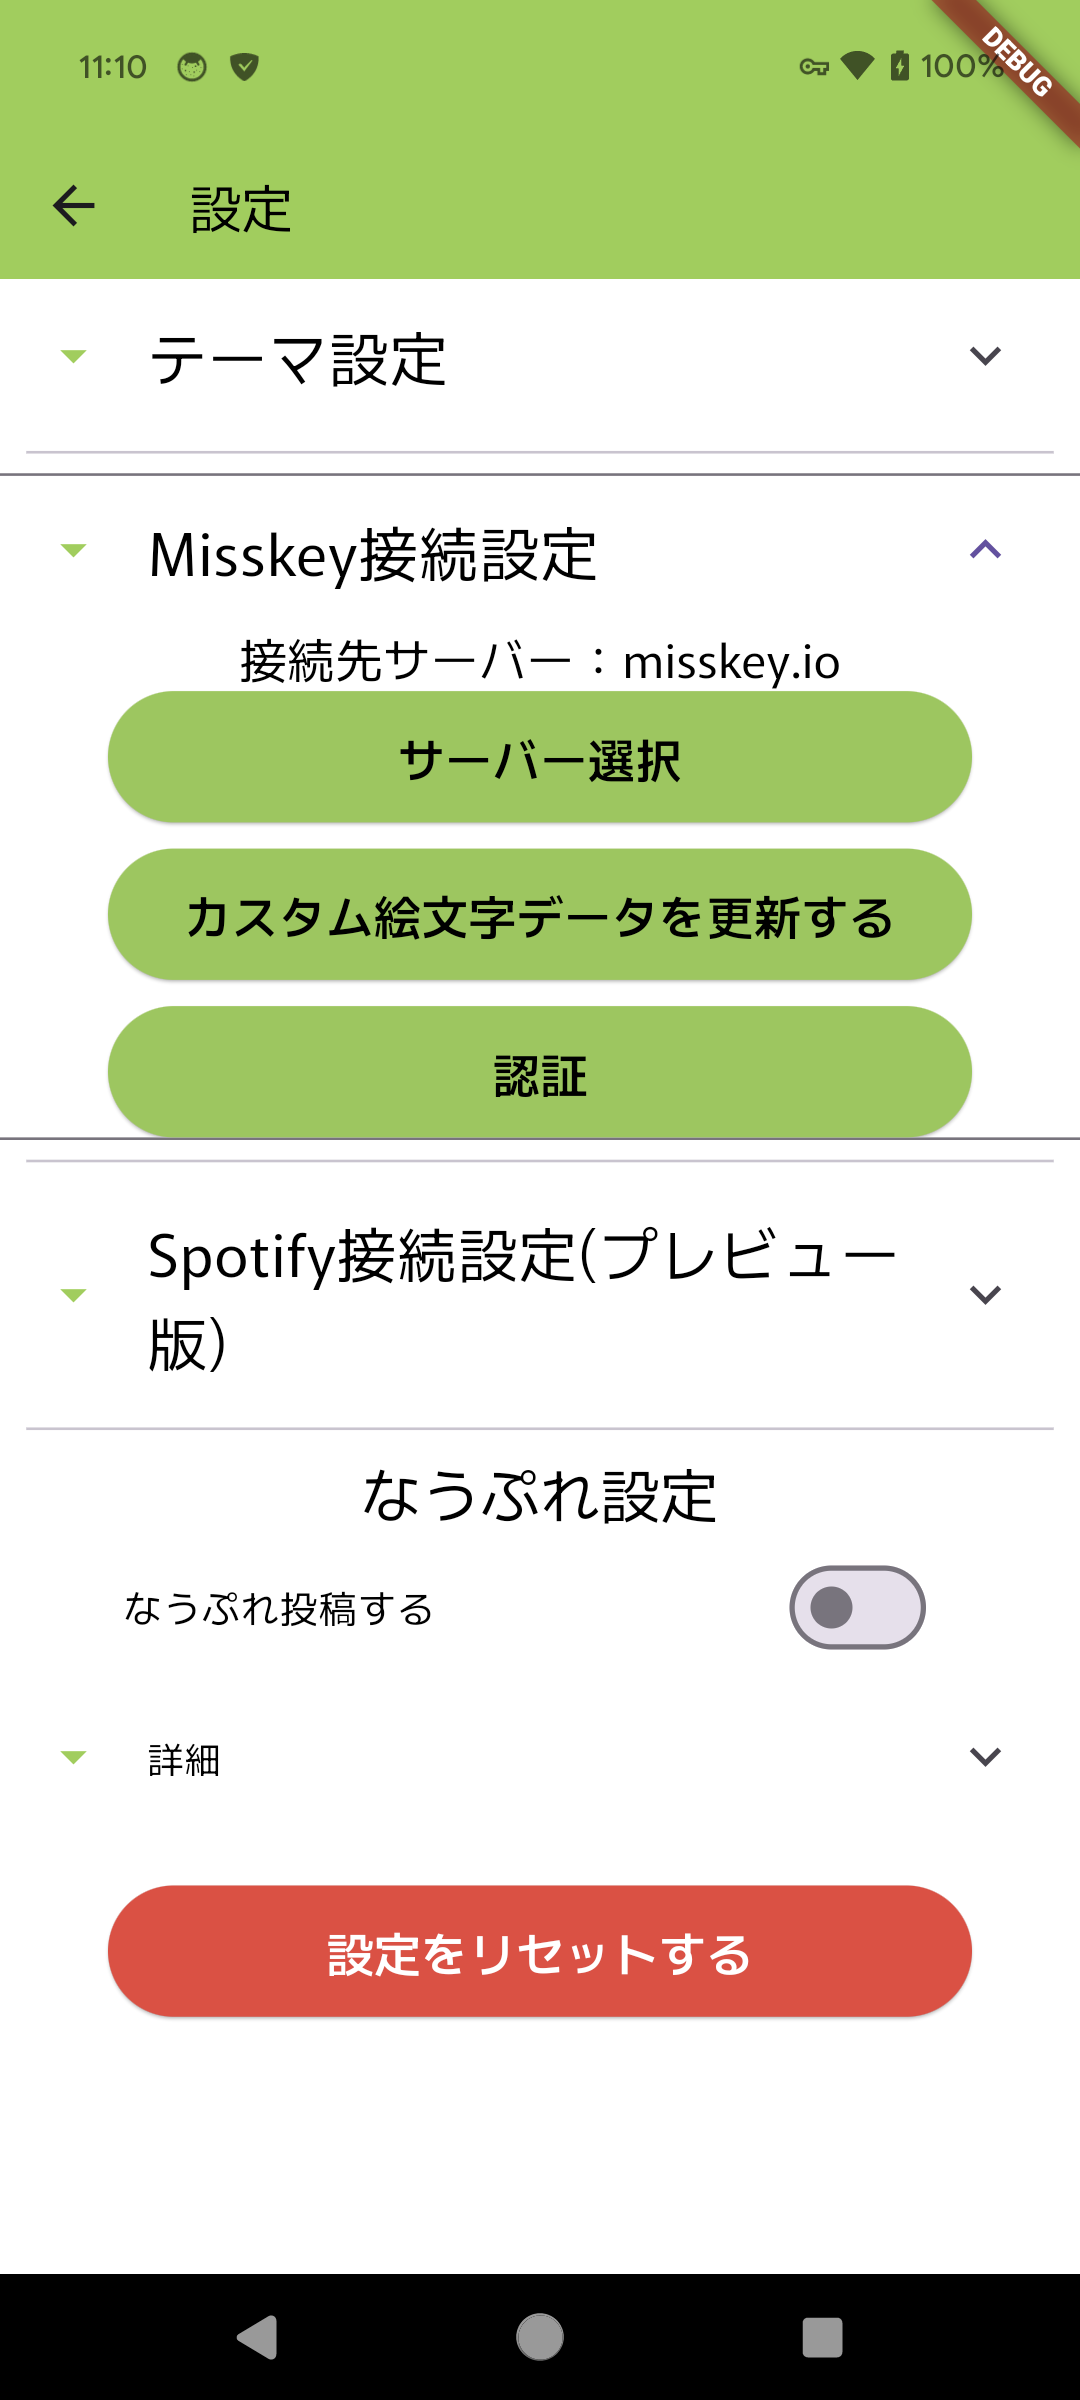
\includegraphics[width=5cm]{./pictures/misskey2.png}
                            }
                            \caption{展開後}
                            \label{img:misskey2}
                        \end{minipage}
                        \caption*{\mi 接続設定(\currentVersion)}
                    \end{figure}

                \item \ttbox{認証}を押下してアプリへのアクセス許可ページにアクセスしてください。
                \label{item:misskey3}

                \newpage
                \item \nowplaying したい\mi アカウントのユーザー名、パスワードを入力して\ttbox{ログイン}を押下してください。
                \label{item:misskey4}
                    \begin{figure}[htbp]
                        \centering
                        \fbox{
                            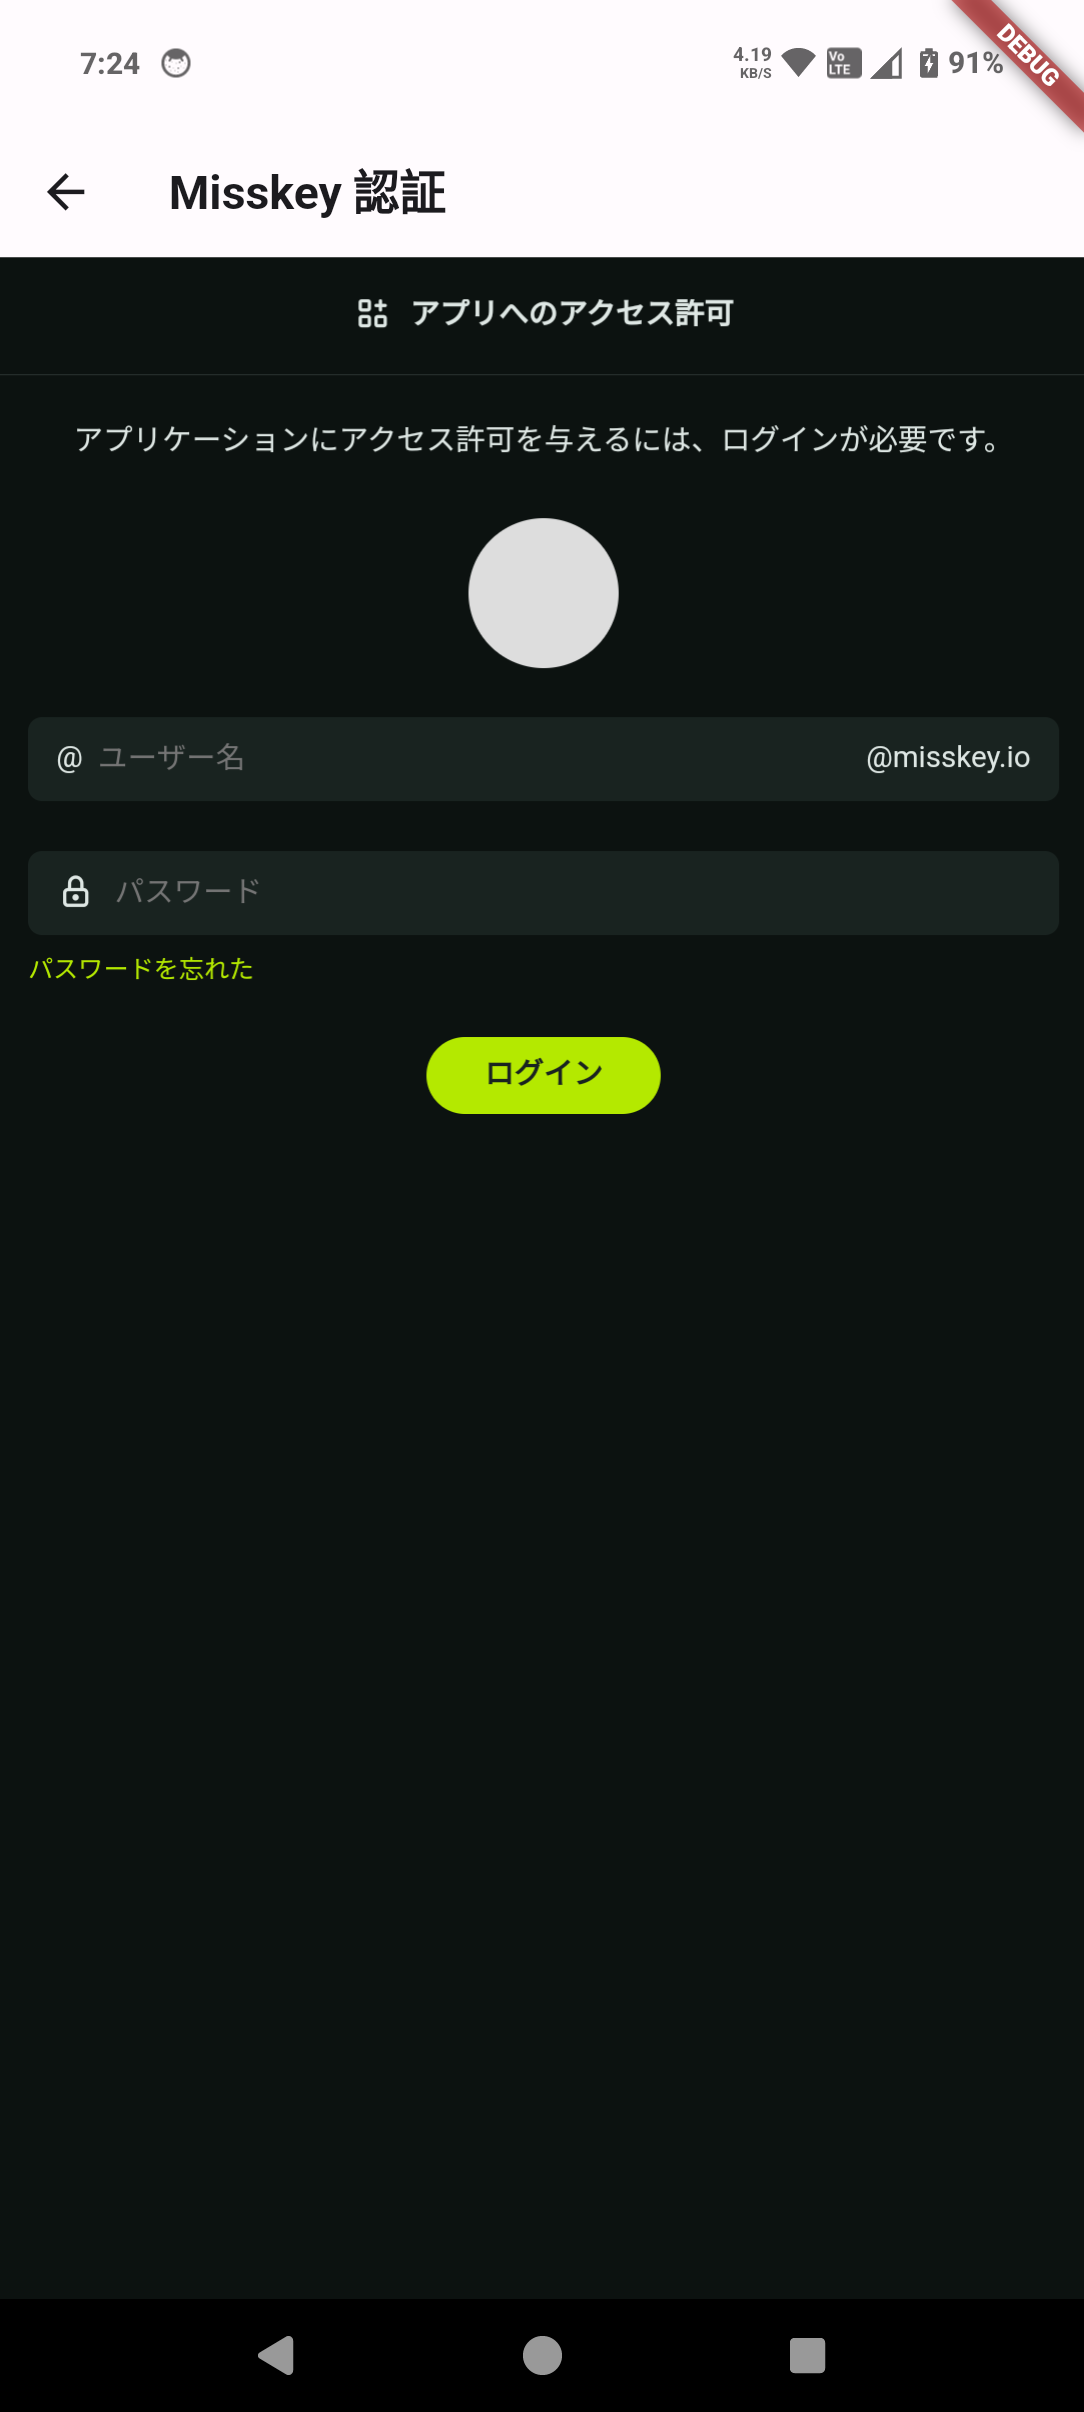
\includegraphics[width=5cm]{./pictures/misskey3.png}
                        }
                        \caption{ログインページ}
                        \label{img:misskey3}
                    \end{figure}

                \newpage
                \item \imageref{img:misskey4}のように二要素認証の入力を要求された場合は、\bracketref{item:misskey1}で作成した認証コードを入力して\ttbox{ログイン}を押下してください。
                    \begin{figure}[htbp]
                        \centering
                        \fbox{
                            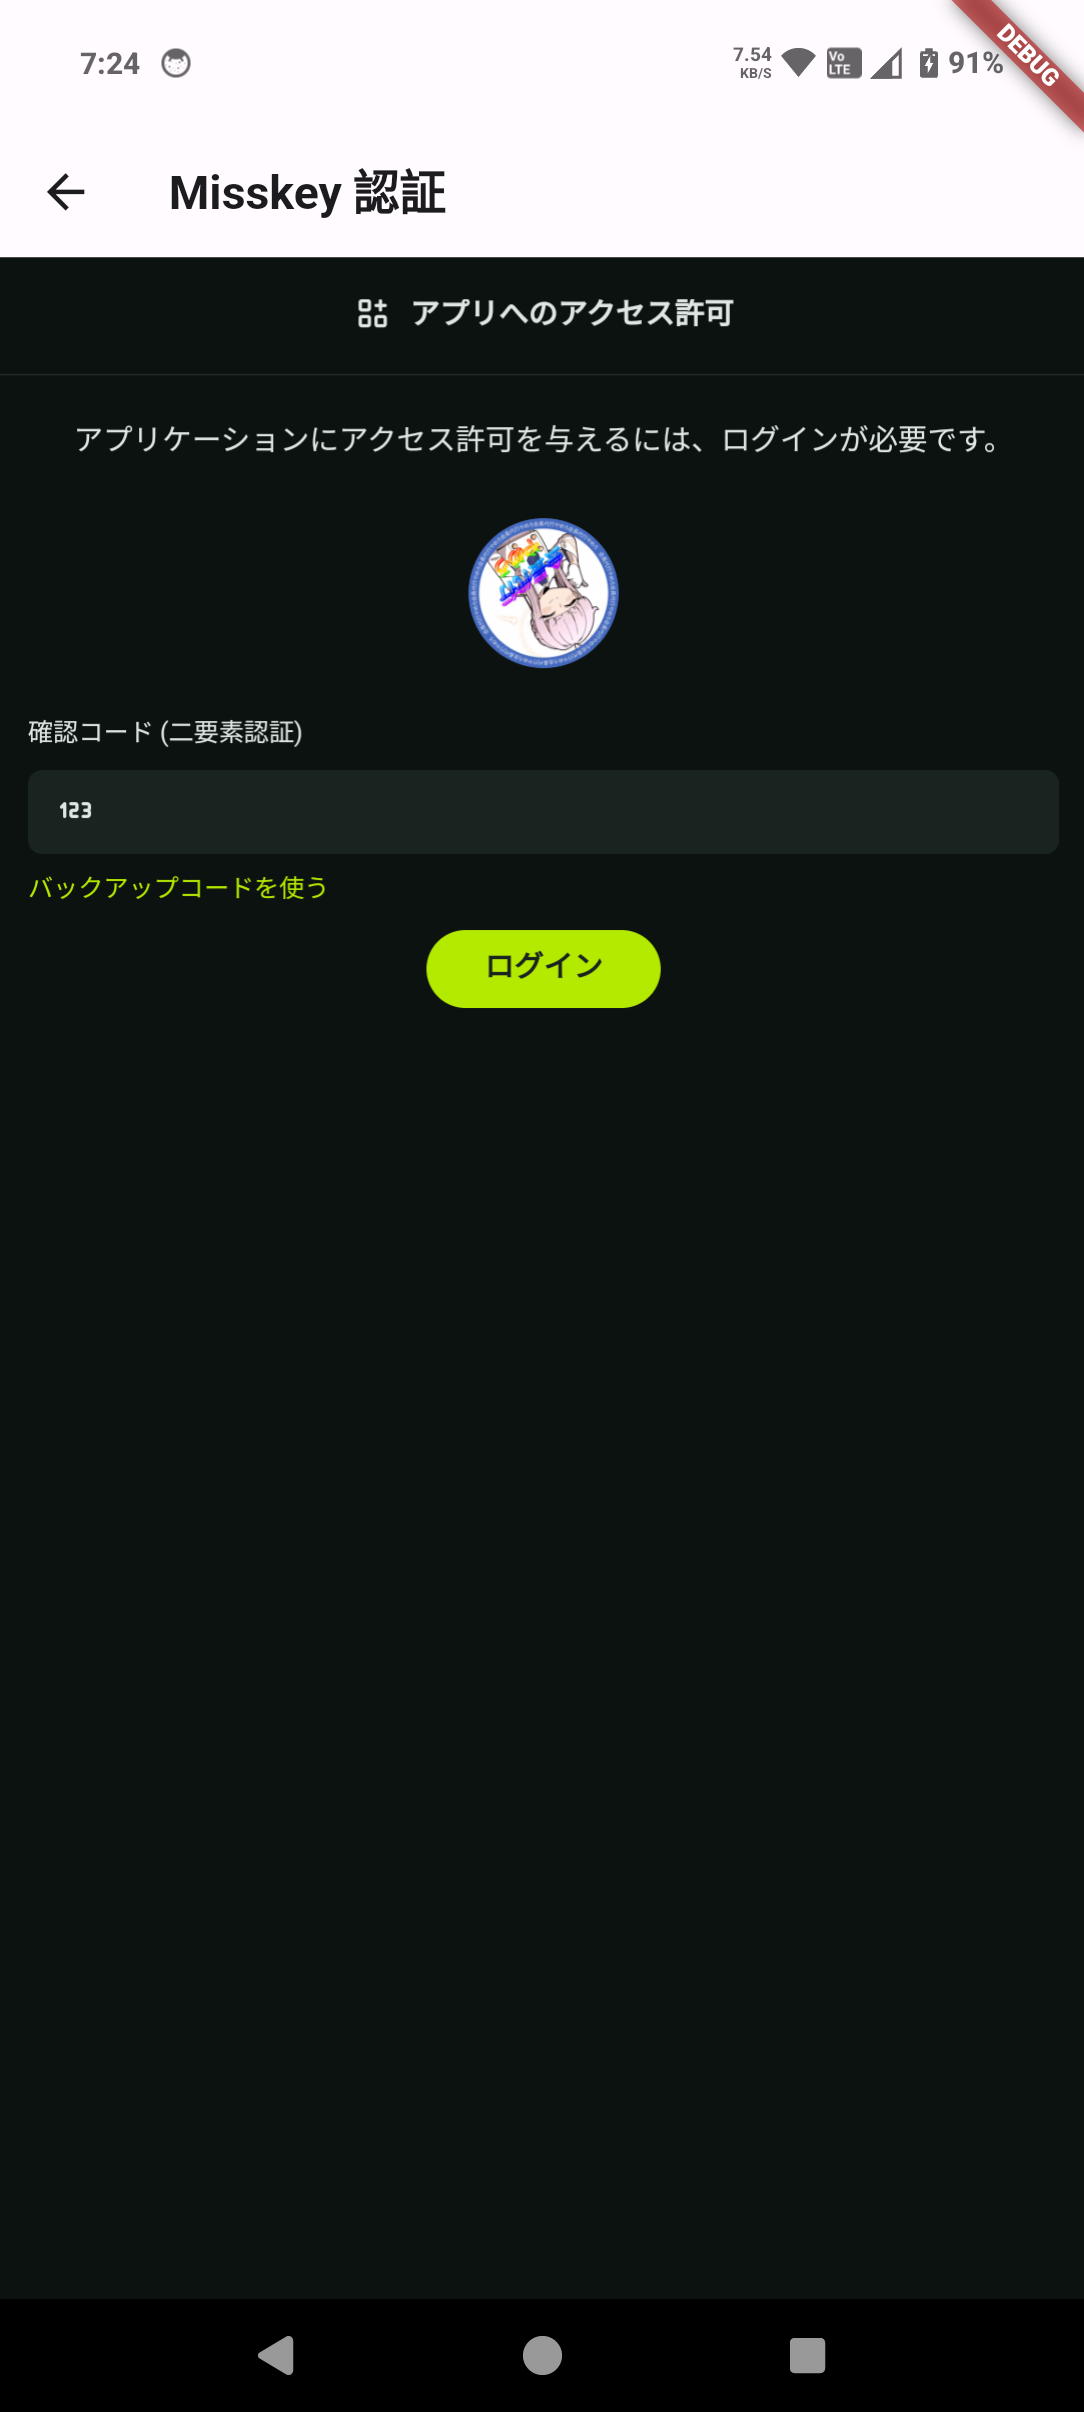
\includegraphics[width=5cm]{./pictures/misskey4.png}
                        }
                        \caption{二要素認証入力ページ}
                        \label{img:misskey4}
                    \end{figure}

                \newpage
                \item \imageref{img:misskey5}のようなアクセス許可ページが表示されるので、\ttbox{許可}を押下してください。
                    \begin{figure}[htbp]
                        \centering
                        \fbox{
                            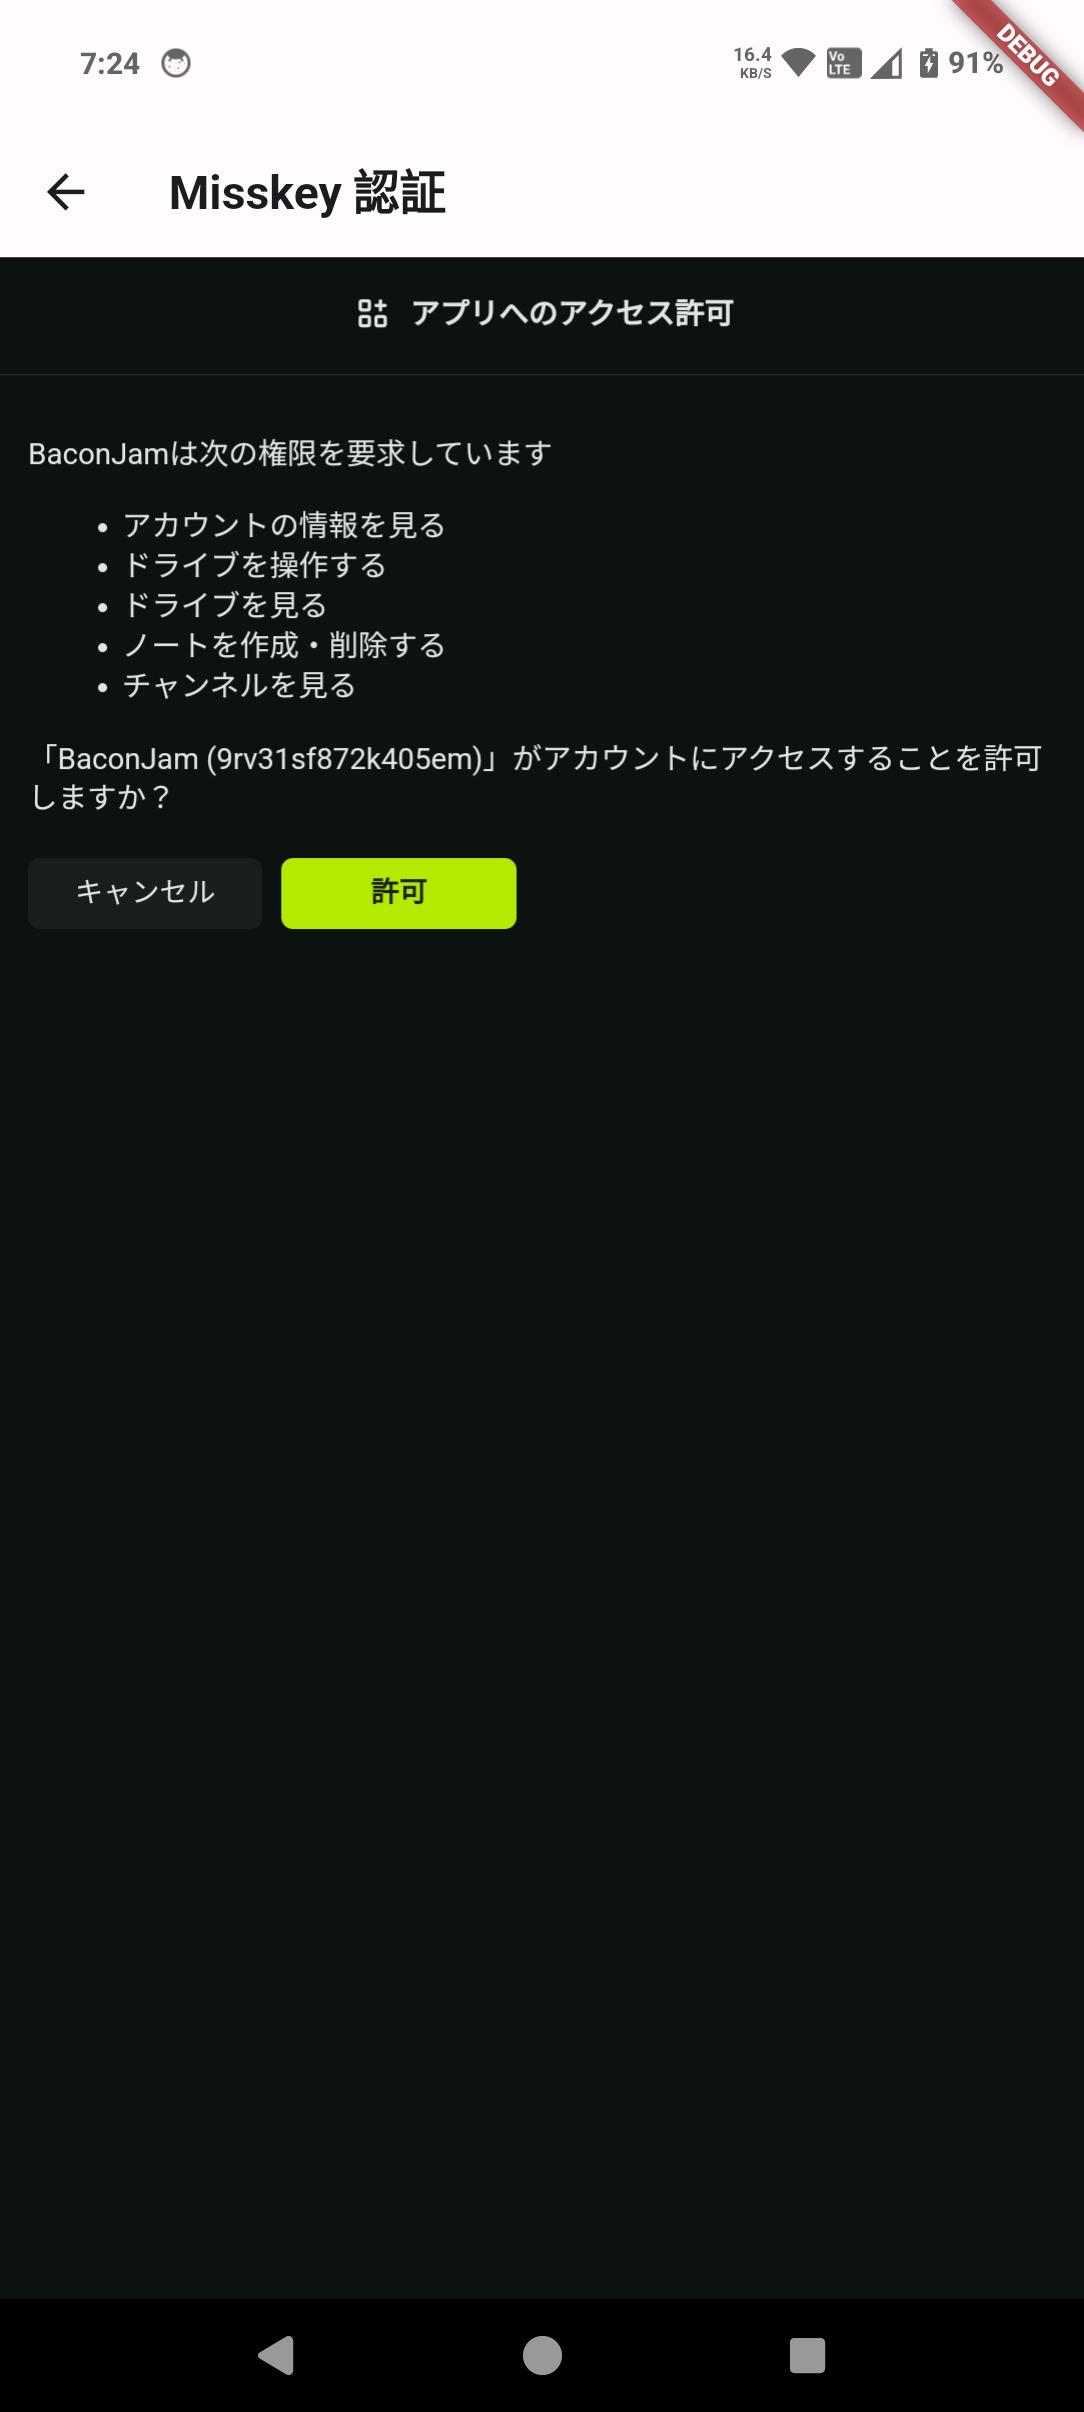
\includegraphics[width=5cm]{./pictures/misskey5.png}
                        }
                        \caption{アクセス許可ページ}
                        \label{img:misskey5}
                    \end{figure}

                \newpage
                \item \imageref{img:misskey6}のような認証完了ページが表示されたら、画面左上の戻るを押下してください。
                    \begin{figure}[htbp]
                        \centering
                        \fbox{
                            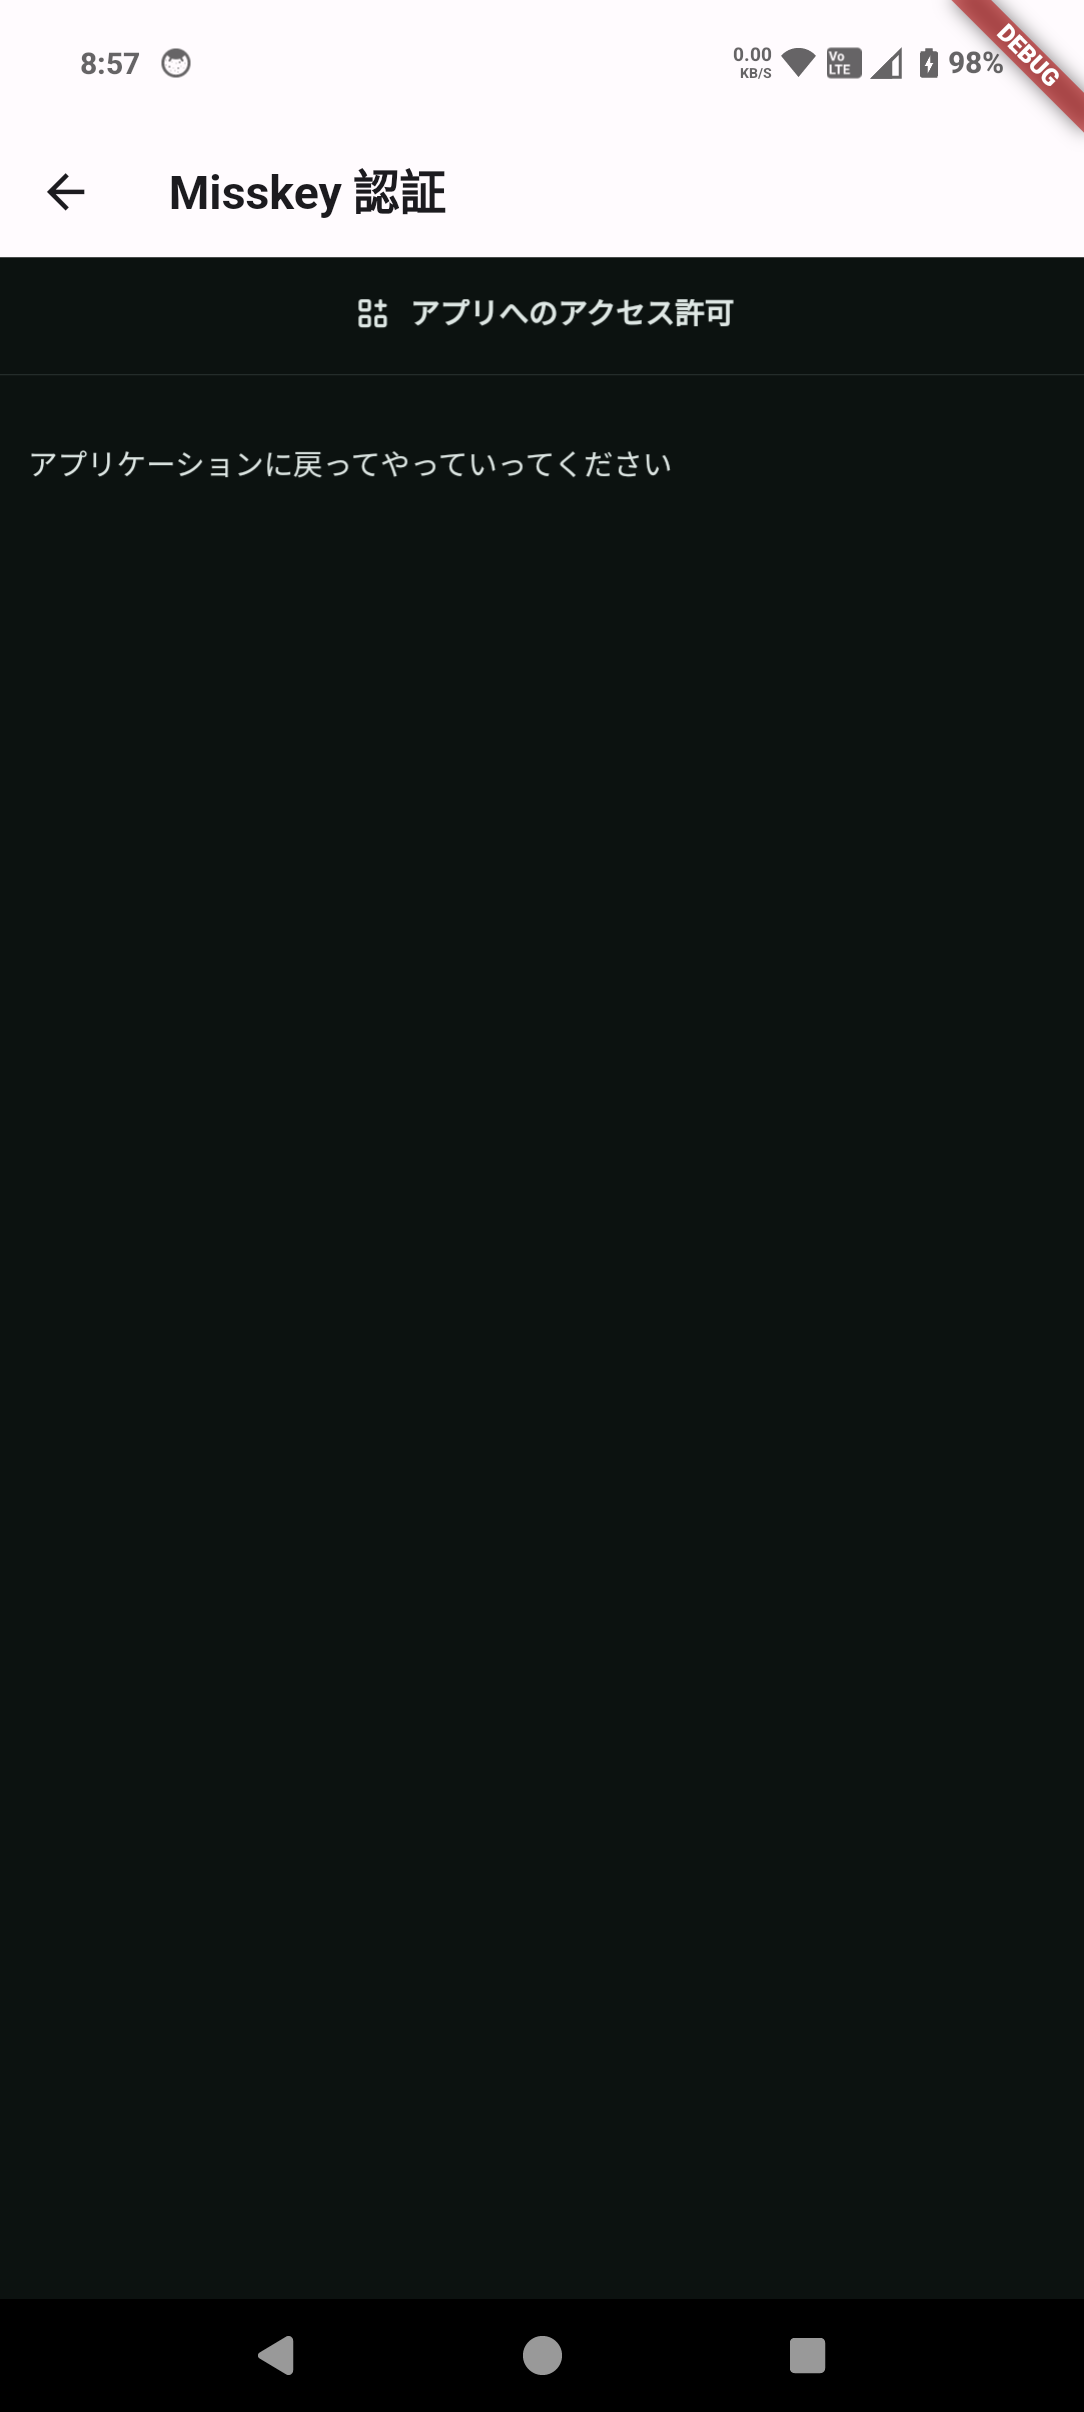
\includegraphics[width=5cm]{./pictures/misskey6.png}
                        }
                        \caption{アクセス許可ページ}
                        \label{img:misskey6}
                    \end{figure}

                \newpage
                \item \imageref{img:misskey7}のようなダイアログが表示され、ご自身のアカウントが正しく連携されていることを確認してください。
                    \begin{figure}[htbp]
                        \centering
                        \fbox{
                            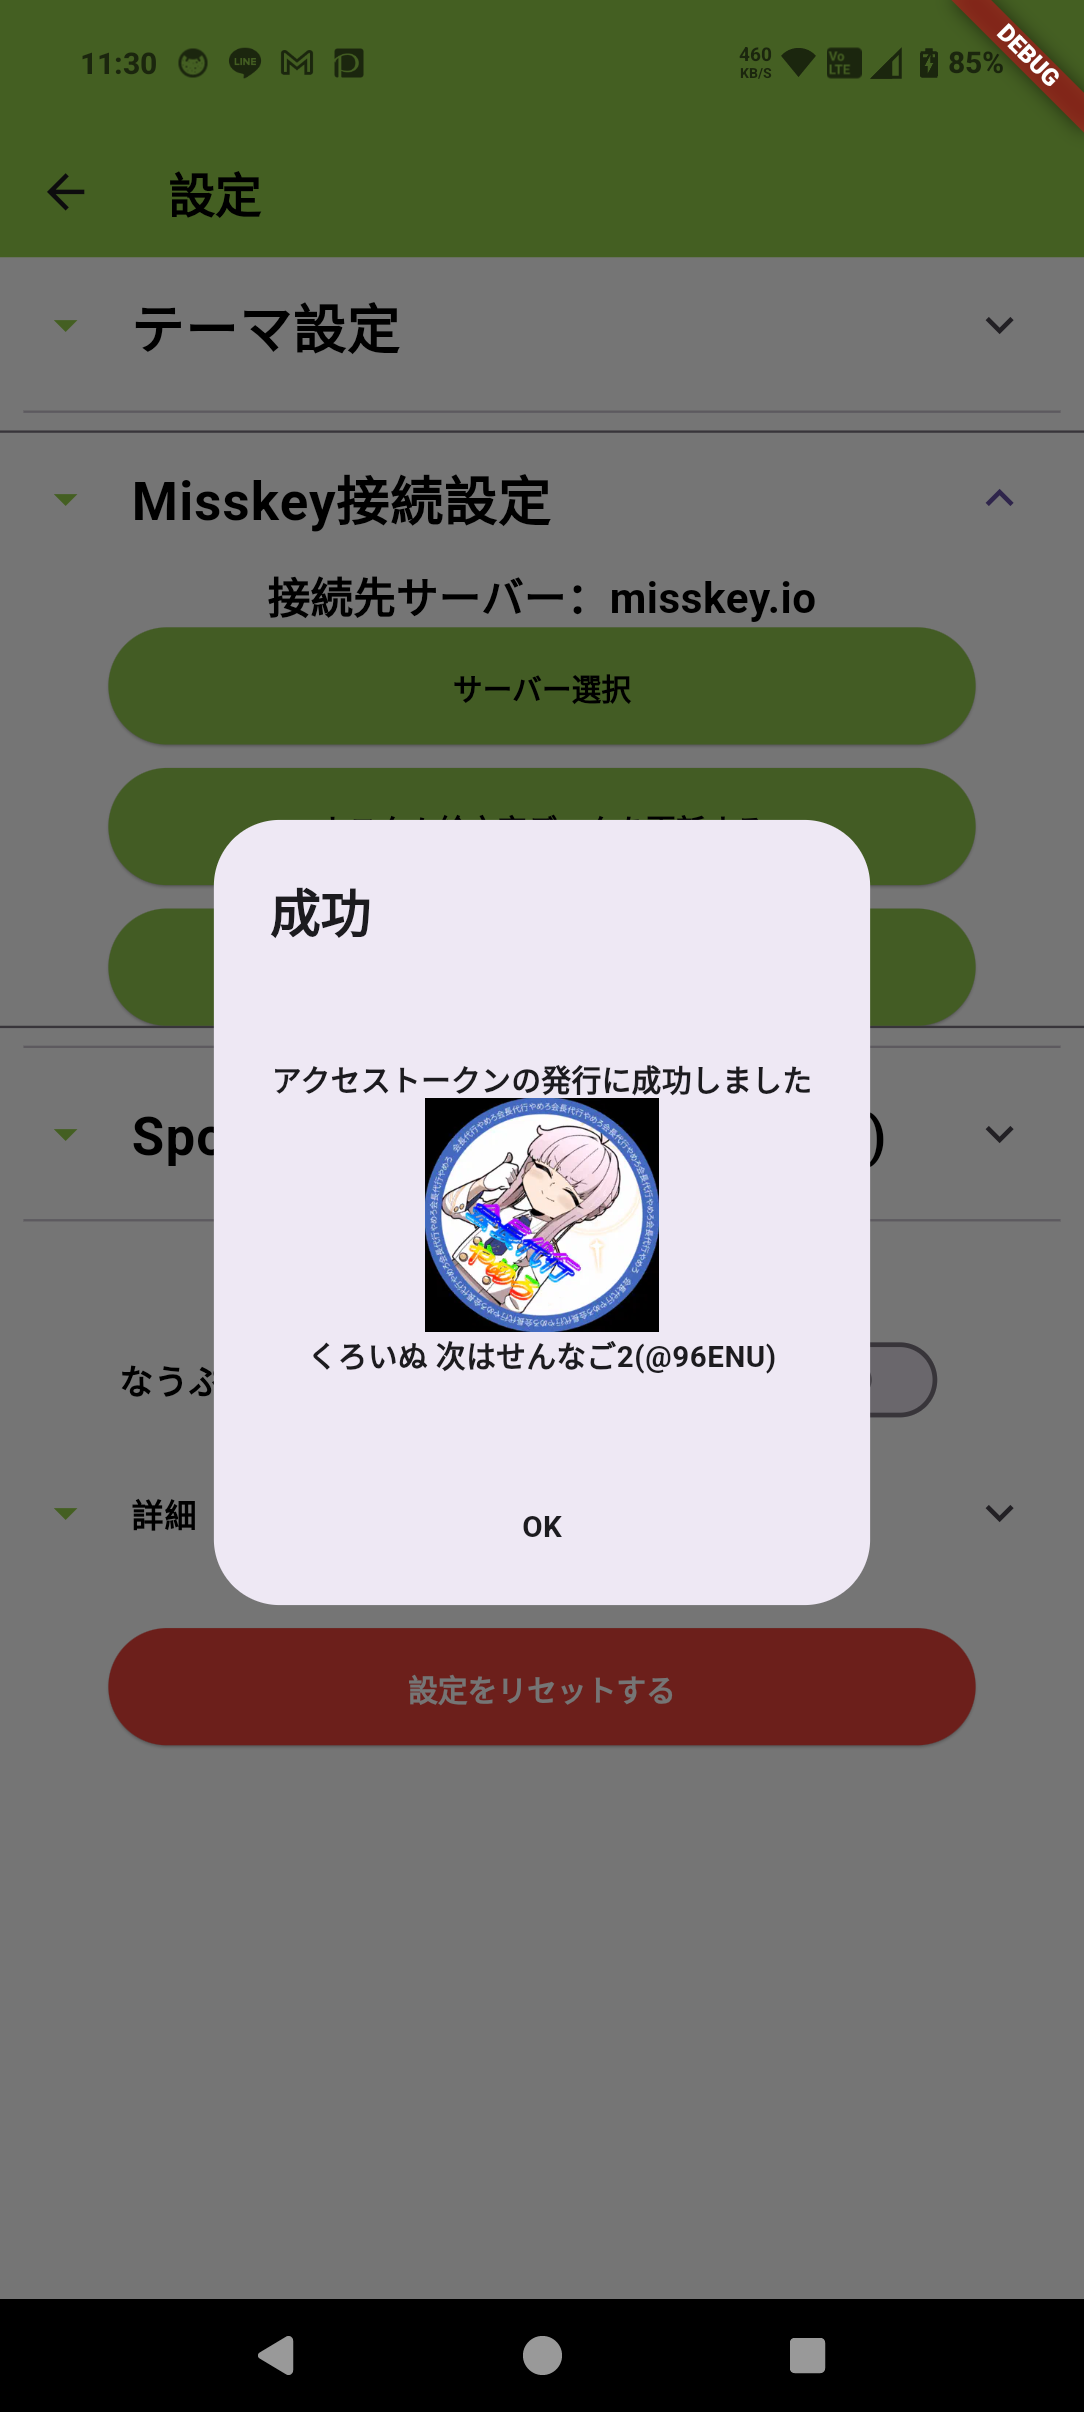
\includegraphics[width=5cm]{./pictures/misskey7.png}
                        }
                        \caption{アプリ連携完了ダイアログ}
                        \label{img:misskey7}
                    \end{figure}
            \end{enumerate}

        \newpage
        \subsubsection{発行した\accessToken の確認・削除}
        \label{sec:misskey4}
            \begin{enumerate}
                \item 連携先の\mi サーバーで\ttbox{設定}→\ttbox{API}を押下してください。
                    \begin{figure}[htbp]
                        \centering
                        \fbox{
                            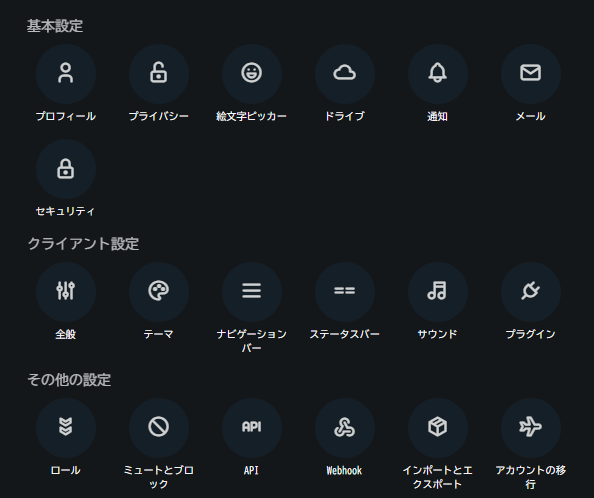
\includegraphics[width=5cm]{./pictures/misskey8.png}
                        }
                        \caption{設定ウィンドウ}
                        \label{img:misskey8}
                    \end{figure}

                \item \ttbox{\accessToken の管理}を押下してください。
                    \begin{figure}[htbp]
                        \centering
                        \fbox{
                            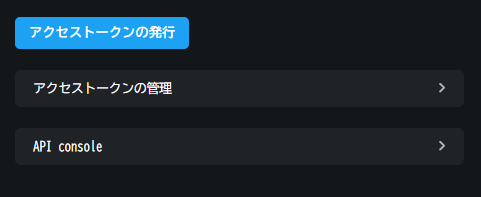
\includegraphics[width=5cm]{./pictures/misskey9.png}
                        }
                        \caption{APIウィンドウ}
                        \label{img:misskey9}
                    \end{figure}

                \item \accessToken 覧に、\bj という名前のものが発行されています。不要になった場合は、ゴミ箱アイコンを押下して\accessToken を削除してください。
                    \begin{figure}[htbp]
                        \centering
                        \fbox{
                            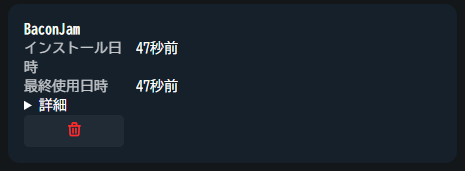
\includegraphics[width=5cm]{./pictures/misskey10.png}
                        }
                        \caption{アクセストークン}
                        \label{img:misskey10}
                    \end{figure}
            \end{enumerate}

\newpage
\section{Spotifyとの連携 \index{spotify@Spotify}}
\label{sec:spotify1}
    \subsection{Spotify側の設定}
    \label{sec:spotify2}
        \subsubsection{Spotify for Developersの認証 \index{spotifyfordevelopers@Spotify for Developers}}
        \label{sec:spotify3}
            \begin{enumerate}
                \item \href{https://developer.spotify.com}{Spotify for Developers}にアクセスし、ご利用のSpotifyアカウントでログインしてください。
                \label{item:spotify1}
                \item アカウント名を押下してメニューを表示し、\ttbox{Dashboard}を押下して\spotifydashboard へ移動してください。
                \label{item:spotify2}
                    \begin{figure}[htbp]
                        \centering
                        \fbox{
                            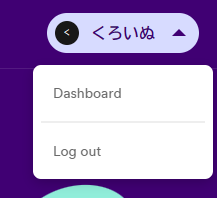
\includegraphics[width=5cm]{./pictures/spotify1.png}
                        }
                        \caption{メニューのDashboard}
                        \label{img:spotify1}
                    \end{figure}

                \item \spotifydashboard で
                    \begin{screen}
                        \texttt{You need to verify your email address (アカウントに登録されているメールアドレス) before you can create an app.}
                    \end{screen}
                    と表示されている部分の\ttbox{Update email address}を押下してください。
                \label{item:spotify3}
                    \begin{figure}[htbp]
                        \centering
                        \fbox{
                            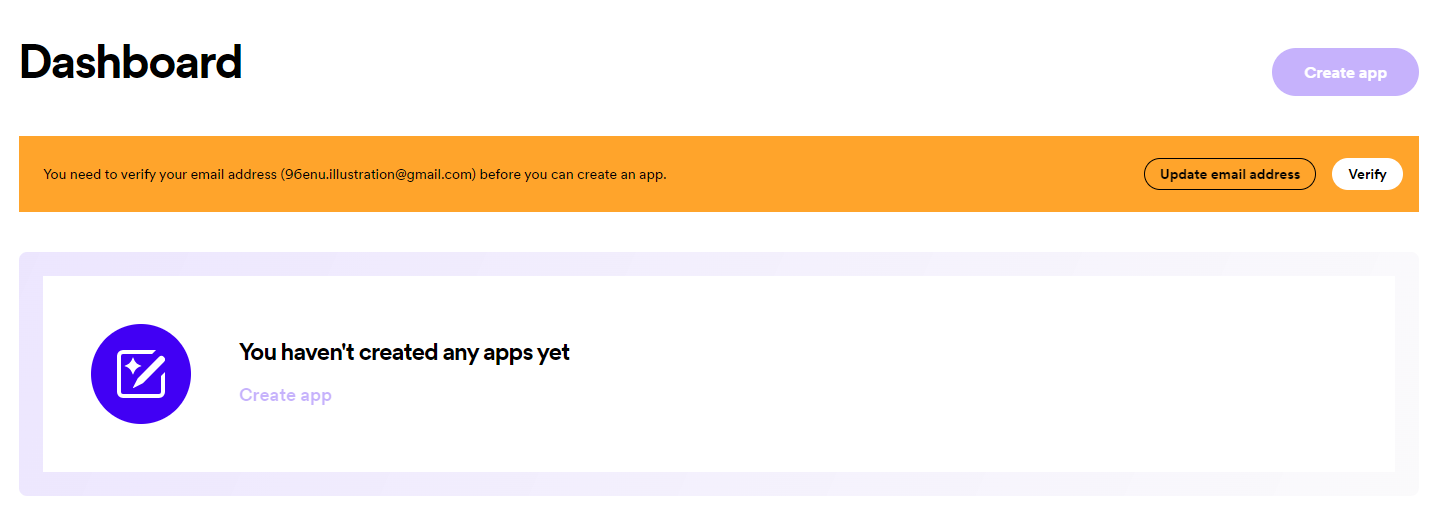
\includegraphics[width=\linewidth]{./pictures/spotify2.png}
                        }
                        \caption{DashboardのUpdate email address}
                        \label{img:spotify2}
                    \end{figure}

                \newpage
                \item \bracketref{item:spotify3}の実行後、アカウントに登録されているメールアドレスに\texttt{no-reply@spotify.com}から\imageref{img:spotify3}のようなセキュリティ確認のメールが送られてくるので、\ttbox{メールアドレスを確認する}を押下してください。
                \label{item:spotify4}
                    \begin{figure}[htbp]
                        \centering
                        \fbox{
                            \includegraphics[width=6cm]{./pictures/Spotify3.png}
                        }
                        \caption{セキュリティ確認のメール}
                        \label{img:spotify3}
                    \end{figure}

                \newpage
                \item ブラウザ上で\imageref{img:spotify4}のようなページが表示されたら、\spotifydashboard に戻ってください。
                \label{item:spotify5}
                    \begin{figure}[htbp]
                        \centering
                        \fbox{
                            \includegraphics[width=6cm]{./pictures/Spotify4.png}
                        }
                            \caption{認証完了画面}
                        \label{img:spotify4}
                    \end{figure}
                \item \spotifydashboard で、\bracketref{item:spotify3}時点では押下できなかった\ttbox{Create app}が押下できるようになっていれば、認証完了です。
            \end{enumerate}

        \newpage
        \subsubsection{Spotifyと\bj 接続用appの作成}
        \label{sec:spotify4}
            \begin{enumerate}
                \item \spotifydashboard の\ttbox{Create app}を押下してください。
                \label{item:spotify6}
                    \begin{figure}[htbp]
                        \centering
                        \fbox{
                            \includegraphics[width=\linewidth]{./pictures/Spotify5.png}
                        }
                        \caption{\spotifydashboard のCreate app}
                        \label{img:spotify5}
                    \end{figure}

                \newpage
                \item \imageref{img:spotify6}のようなapp作成ページが表示されるので、以下を参考に値を設定してください。
                \label{item:spotify7}
                    \begin{figure}[htbp]
                        \centering
                        \fbox{
                            \includegraphics[width=\linewidth]{./pictures/Spotify6.png}
                        }
                        \caption{app作成ページ}
                        \label{img:spotify6}
                    \end{figure}
                    \begin{itemize}
                        \item[\texttt{App name}] なんらかの値を設定してください\footnote{自由な値で構いませんが、\bj 用のappであることが分かるような名前の設定を推奨します。}。
                        \item[\texttt{App description}] なんらかの値を設定してください。
                        \item[\texttt{Website}] 空欄で構いません。
                        \item[\texttt{Redirect URIs}] 必ず\texttt{http://localhost}という値を設定してください。
                        \item[\texttt{Bundle IDs}] 空欄で構いません。
                        \item[\texttt{Android packages}] 空欄で構いません。
                        \item[\texttt{APIs used}] 以下にチェックを入れてください。
                            \begin{itemize}
                                \item \texttt{Android}
                                \item \texttt{Web API}
                            \end{itemize}
                    \end{itemize}

                \newpage
                \item \bracketref{item:spotify7}の項目設定が完了したら、
                \label{item:spotify8}
                    \begin{screen}
                        \texttt{I understand and agree with Spotify's Developer Terms of Service and Design Guidelines}
                    \end{screen}
                    にチェックを入れ、\ttbox{save}を押下してください。

                \item \imageref{img:spotify7}のようなapp Homeページが表示されたら、作成完了です。
                \label{item:spotify9}
                    \begin{figure}[htbp]
                        \centering
                        \fbox{
                            \includegraphics[width=\linewidth]{./pictures/Spotify7.png}
                        }
                        \caption{app Homeページ}
                        \label{img:spotify7}
                    \end{figure}
            \end{enumerate}

        \newpage
        \subsubsection{接続に必要な情報の取得}
        \label{sec:spotify5}
            \begin{enumerate}
                \item \ref{sec:spotify4}で作成したappのHomeページにアクセスし、\ttbox{Settings}を押下してBasic Informationページに移動してください。
                \label{item:spotify10}

                \item ページ上部の\texttt{Client ID}が表示されている枠の\texttt{View client secret}を押下して、\texttt{Client secret}を表示してください。
                \label{item:spotify11}
                    \begin{figure}[htbp]
                        \centering
                        \fbox{
                            \includegraphics[width=\linewidth]{./pictures/Spotify8.png}
                        }
                        \caption{Basic Informationページ上部(Client secretを表示する前)}
                        \label{img:spotify8}
                    \end{figure}
                    \begin{figure}[htbp]
                        \centering
                        \fbox{
                            \includegraphics[width=\linewidth]{./pictures/Spotify9.png}
                        }
                        \caption{Basic Informationページ上部(Client secretを表示した後)}
                        \label{img:spotify9}
                    \end{figure}

                \item 以下の項目を控えてください。
                \label{item:spotify12}
                    \begin{itemize}
                        \item \texttt{Client ID}
                        \item \texttt{Client secret}
                    \end{itemize}
            \end{enumerate}

            \begin{itembox}[c]{\ttbox{!注意!}}
                \texttt{Client ID},\texttt{Client secret}は他人に知られないように管理してください。アカウントへの不正アクセス・乗っ取り等が発生する危険があります。
            \end{itembox}

    \newpage
    \subsection{\bj 側の設定}
    \label{sec:spotify6}
        \begin{enumerate}
            \item 設定画面の\ttbox{Spotify接続設定(プレビュー版)}を押下して、設定項目を展開してください。
                \begin{figure}[htbp]
                    \begin{minipage}[b]{0.45\linewidth}
                        \centering
                        \fbox{
                            \includegraphics[width=5cm]{./pictures/Spotify10.png}
                        }
                        \caption{展開前}
                        \label{img:spotify10}
                    \end{minipage}
                    \begin{minipage}[b]{0.45\linewidth}
                        \centering
                        \fbox{
                            \includegraphics[width=5cm]{./pictures/Spotify11.png}
                        }
                        \caption{展開後}
                        \label{img:spotify11}
                    \end{minipage}
                    \caption*{Spotify接続設定(\currentVersion)}
                \end{figure}

            \newpage
            \item \ref{sec:spotify5} \bracketref{item:spotify12}で控えた\texttt{Client ID},\texttt{Client secret}を\ttbox{Spotify接続設定(プレビュー版)}に入力してください。
                \begin{figure}[htbp]
                    \centering
                    \fbox{
                        \includegraphics[width=5cm]{./pictures/Spotify12.png}
                    }
                    \caption{\texttt{Client ID},\texttt{Client secret}を入力}
                    \label{img:spotify12}
                \end{figure}

            \newpage
            \item \ttbox{Spotify接続設定(プレビュー版)}の\ttbox{接続テスト}ボタンが押下できるようになるので、押下して認証ページへアクセスしてください。
            \item \imageref{img:spotify13}のような認証ページが表示されるので、\ttbox{同意する}を押下してください。
                \begin{figure}[htbp]
                    \centering
                    \fbox{
                        \includegraphics[width=5cm]{./pictures/Spotify13.png}
                    }
                    \caption{認証ページ}
                    \label{img:spotify13}
                \end{figure}

            \newpage
            \item 認証ページが閉じ、\imageref{img:spotify14}のような成功ダイアログが表示されたらSpotify側の準備は完了です\footnote{ダイアログ内のユーザー名がご自身のアカウントと一致していることを確認してください}。
                \begin{figure}[htbp]
                    \centering
                    \fbox{
                        \includegraphics[width=5cm]{./pictures/Spotify14.png}
                    }
                    \caption{認証ページ}
                    \label{img:spotify14}
                \end{figure}
        \end{enumerate}

    \newpage
    \subsection{Spotify連携時の挙動について}
    \label{sec:spotify7}
    \begin{itemize}
        \item 約1分に一度、Spotifyで再生中の曲を確認し\mi への\nowplaying を行います。
        \item 以下のいずれかに該当する場合、\nowplaying を行いません。
        \begin{itemize}
            \item 再生中の曲がない
            \item \mi の\accessToken が設定されていない
            \item \nowplaying が有効になっていない
            \item 前回の\nowplaying と曲名・アーティスト名が変化していない
            \item スマートフォンがネットワークに接続されていない
            \item スマートフォンがロック状態になっている\footnote{ディスプレイを常時表示設定にすることで、解決する場合があります}
        \end{itemize}
    \end{itemize}


\newpage
\section{YouTube接続設定 \index{youtube@YouTube}}
YouTubeとの接続には、\lastfm というサービスと、そこへ再生履歴を反映するための「Scrobble」という機能をもつアプリの2つが必要です。
    \begin{figure}[htbp]
        \centering
        \fbox{
            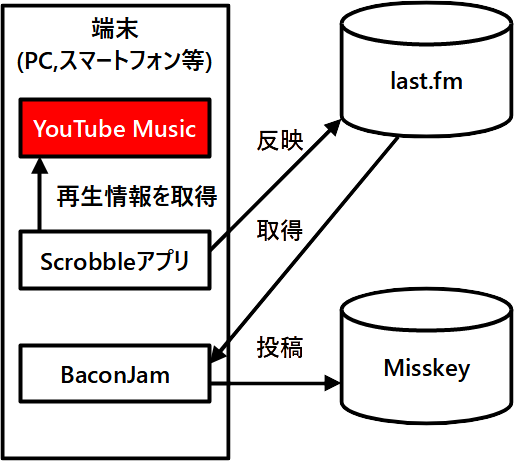
\includegraphics[width=10cm]{./pictures/lastfm1.png}
        }
        \caption{YouTubeとの連携イメージ図}
        \label{img:lastfm1}
    \end{figure}

    \newpage
    \subsection{\lastfm 側の設定}
        \begin{enumerate}
            \item アカウントをお持ちでない場合は、\href{https://www.last.fm}{last.fm}にアクセスし、アカウントを作成してください。
            \item \href{https://www.last.fm/api}{Last.fm Music Discovery API}にアクセスし、\href{https://www.last.fm/api/account/create}{Get an API account}を押下してください。
                \begin{figure}[htbp]
                    \centering
                    \fbox{
                        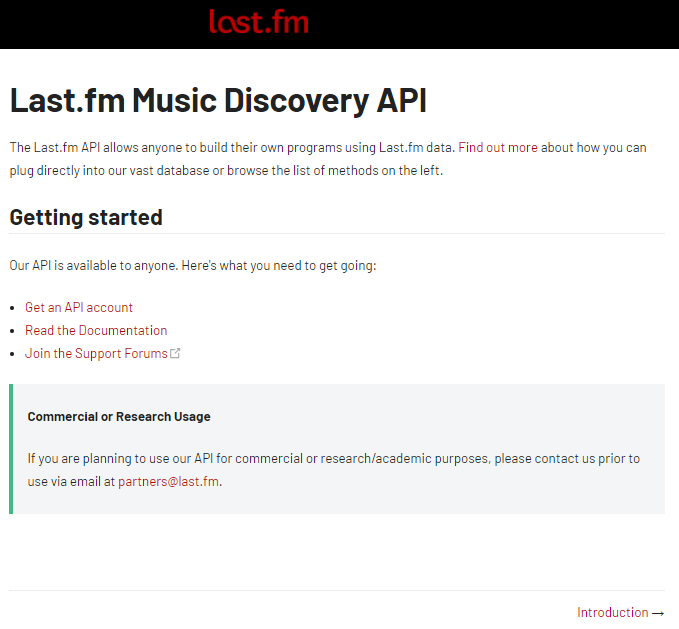
\includegraphics[width=8cm]{./pictures/lastfm2.png}
                    }
                    \caption{Last.fm Music Discovery API}
                    \label{img:lastfm2}
                \end{figure}

            \newpage
            \item APIアカウント作成ページが表示されるので、以下を参考に値を設定して\ttbox{SUBMIT}を押下してください。
                \begin{figure}[htbp]
                    \centering
                    \fbox{
                        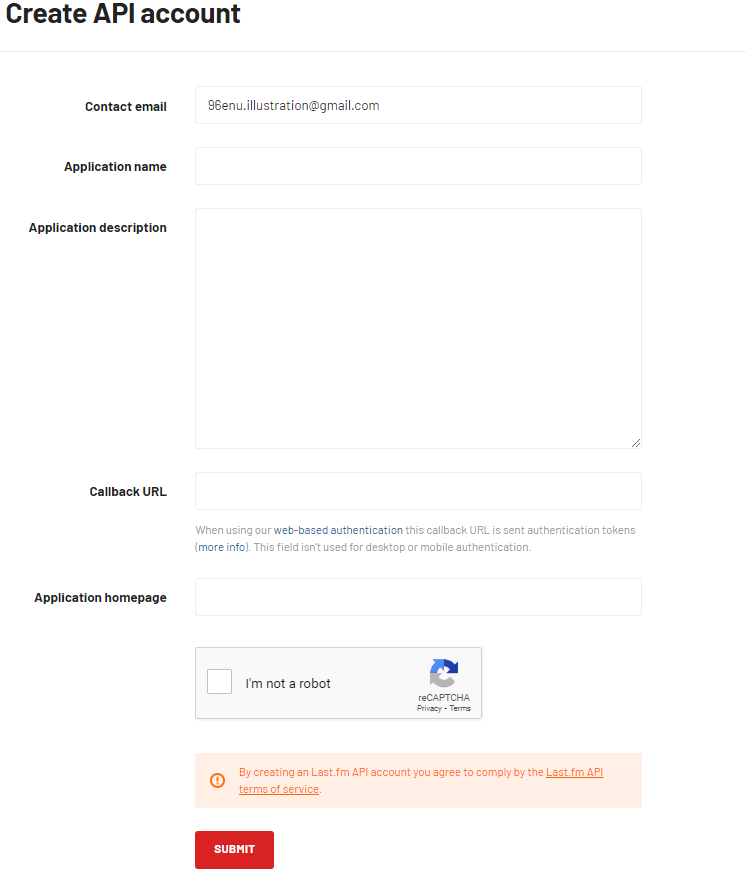
\includegraphics[width=8cm]{./pictures/lastfm3.png}
                    }
                    \caption{APIアカウント作成ページ}
                    \label{img:lastfm3}
                \end{figure}
                \begin{itemize}
                    \item \texttt{Contact email}…last.fmアカウント作成時に使用したメールアドレスが初期設定されているので、そのままで構いません。
                    \item \texttt{Application name}…なんらかの値を設定してください\footnote{自由な値で構いませんが、\bj 用のappであることが分かるような名前の設定を推奨します。}。
                    \item \texttt{Application description}…空欄で構いません。
                    \item \texttt{Callback URL}…空欄で構いません。
                    \item \texttt{Application homepage}…空欄で構いません。
                \end{itemize}

            \newpage
            \item \imageref{img:lastfm4}のようなページに切り替わったら、APIアカウントが正しく作成されています。このページの\texttt{API key}の値を控えてください\footnote{値を忘れてしまった場合は、\href{https://www.last.fm/api/accounts}{APIアプリケーション一覧ページ}で再度確認してください。}。
                \begin{figure}[htbp]
                    \centering
                    \fbox{
                        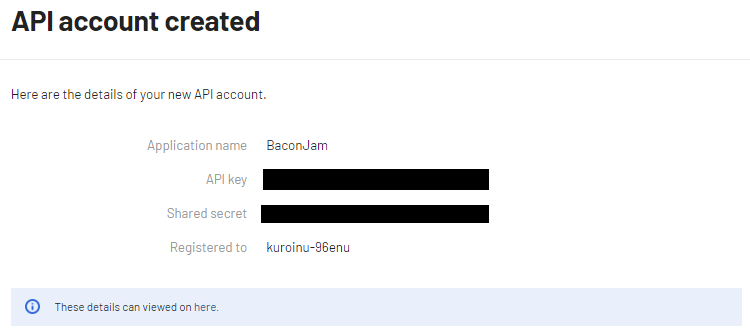
\includegraphics[width=8cm]{./pictures/lastfm4.png}
                    }
                    \caption{APIアカウント作成完了ページ}
                    \label{img:lastfm4}
                \end{figure}
        \end{enumerate}

    \newpage
    \subsection{連携用アプリの設定}
        ここでは、\href{https://play.google.com/store/apps/details?id=com.arn.scrobble&hl=ja&gl=US}{Pano Scrobbler}を使用した場合について解説します。
        \begin{enumerate}
            \item スマートフォンに\href{https://play.google.com/store/apps/details?id=com.arn.scrobble&hl=ja&gl=US}{Pano Scrobbler}をインストールしてください。
            \item Pano Scrobblerを起動して\ttbox{Last.fm}を押下してログインし、\ttbox{YES, ALLOW ACCESS}を押下してください。
                \begin{figure}[htbp]
                    \begin{minipage}[b]{0.45\linewidth}
                        \centering
                        \fbox{
                            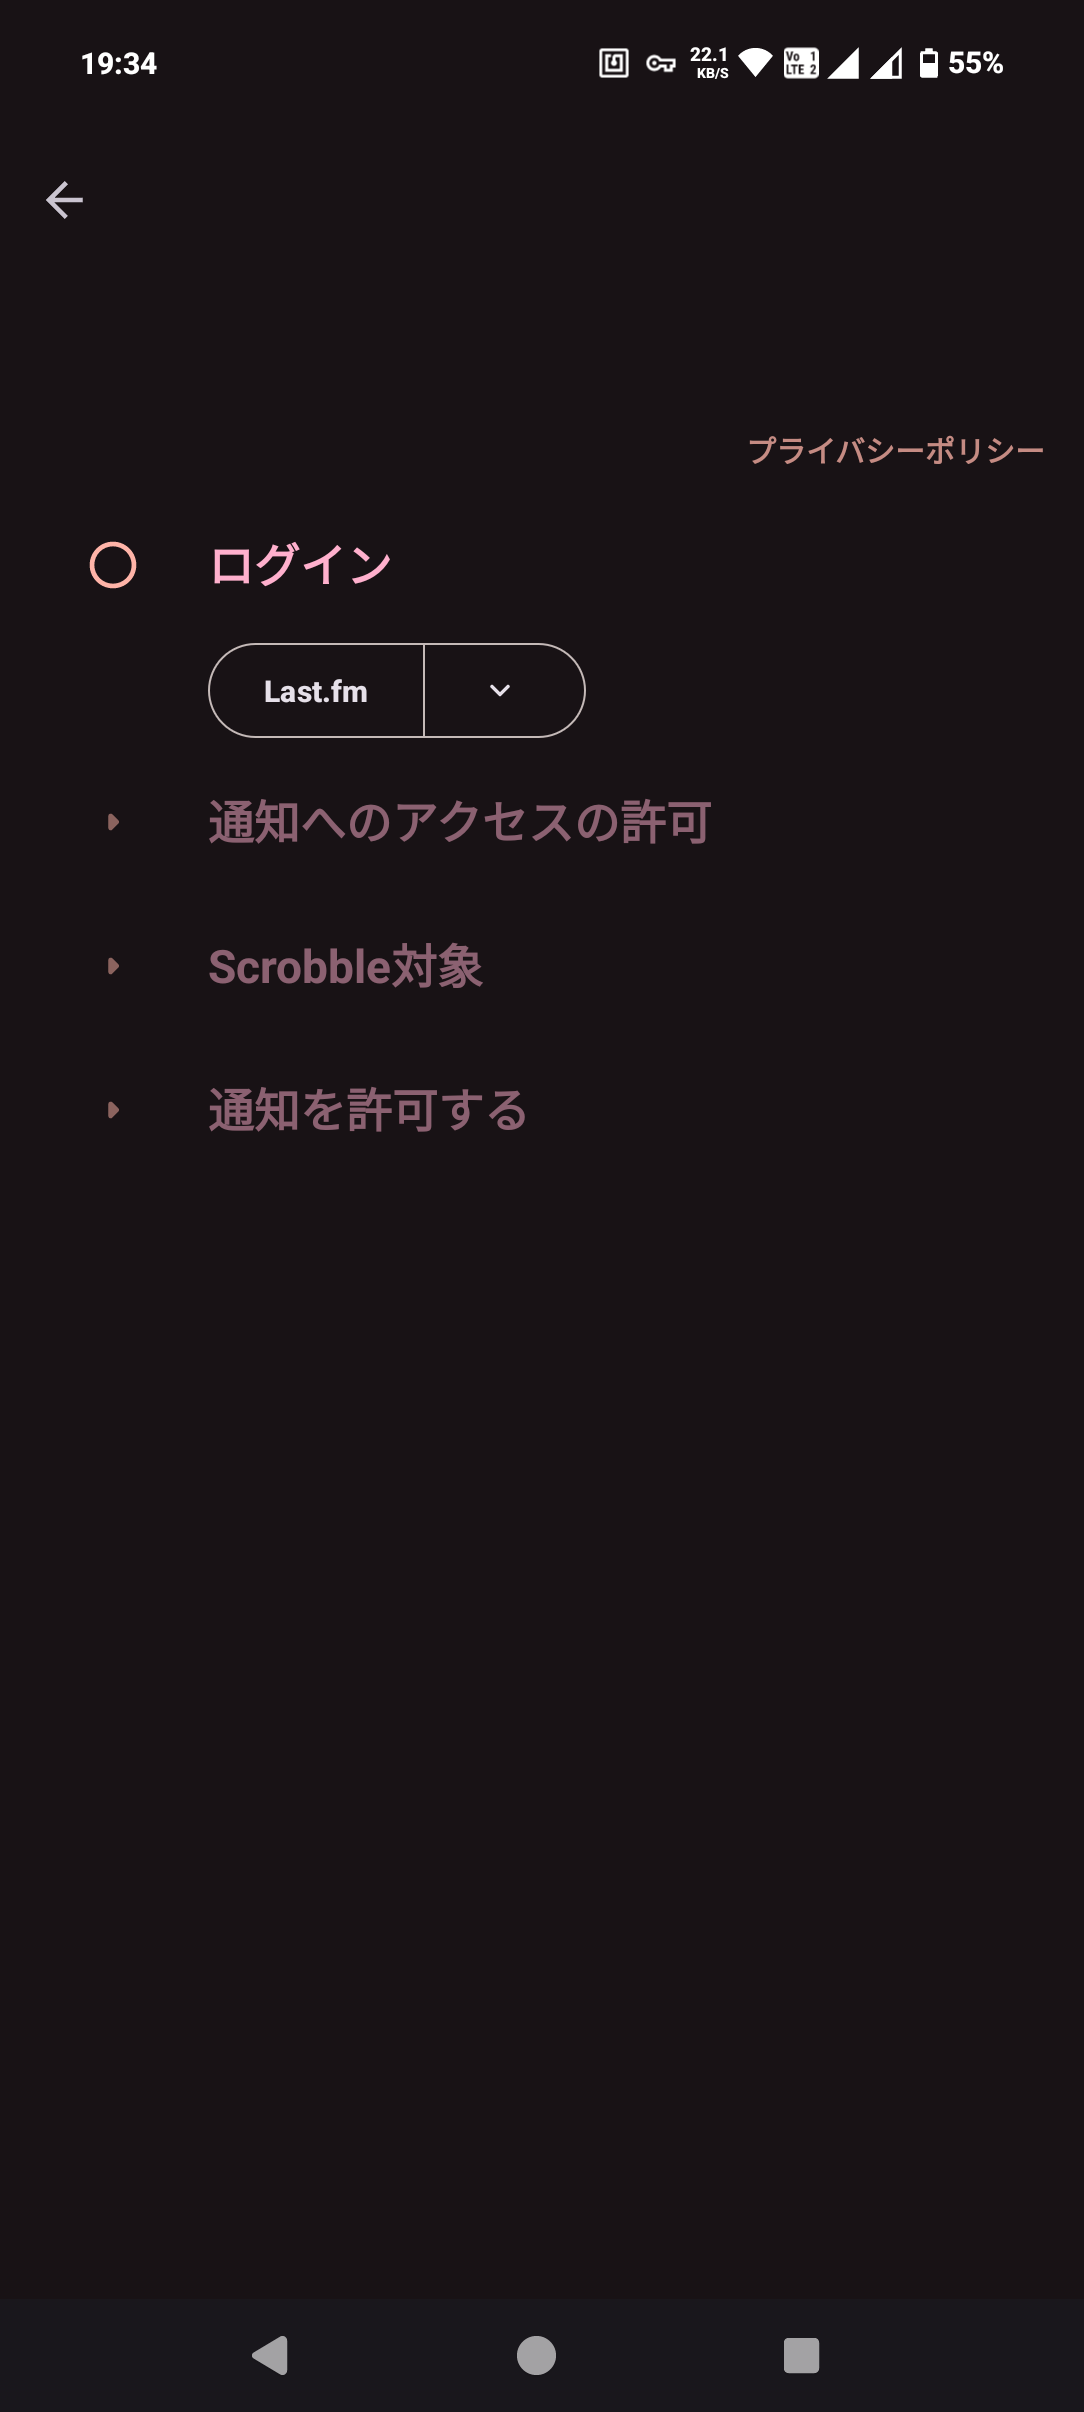
\includegraphics[width=5cm]{./pictures/lastfm5.png}
                        }
                        \label{img:lastfm5}
                    \end{minipage}
                    \begin{minipage}[b]{0.45\linewidth}
                        \centering
                        \fbox{
                            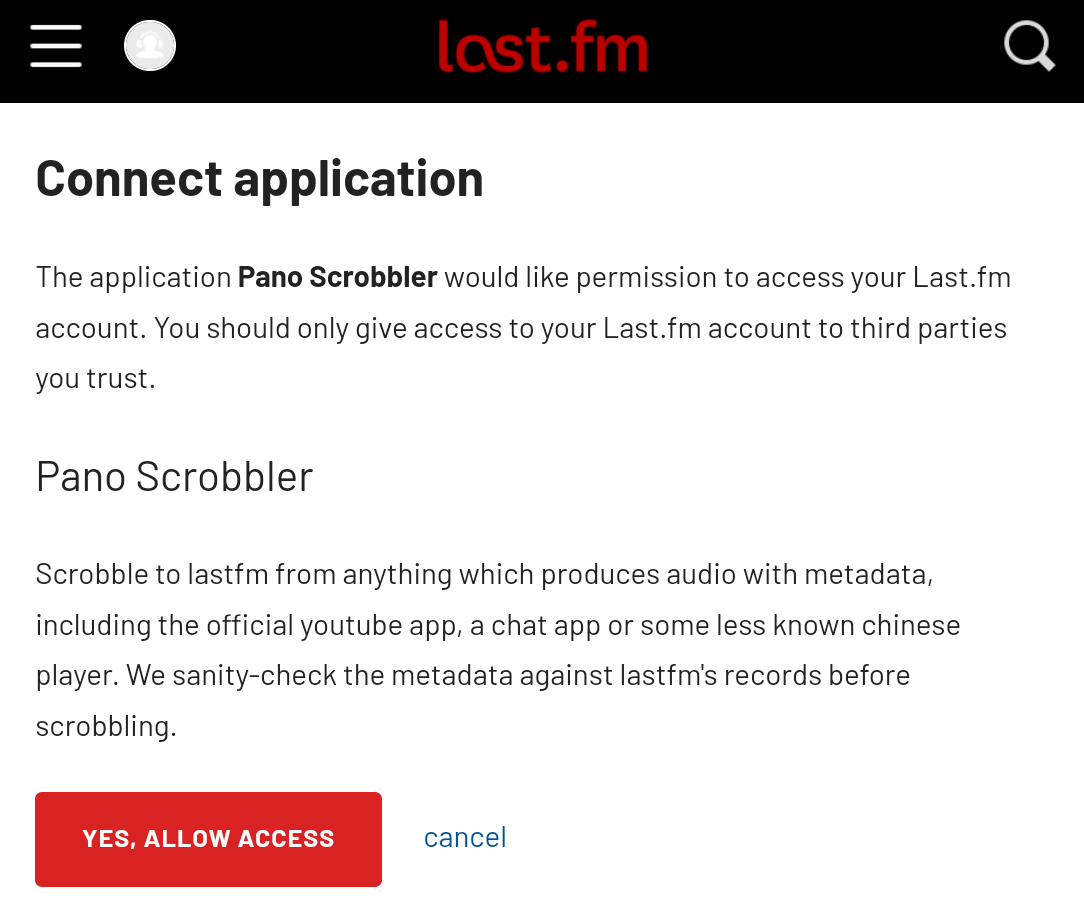
\includegraphics[width=5cm]{./pictures/lastfm6.png}
                        }
                        \label{img:lastfm6}
                    \end{minipage}
                    \caption*{ログイン}
                \end{figure}

            \newpage
            \item 通知へのアクセスを許可してください。
            \item Scrobble対象の\ttbox{開く}を押下して、YouTube Musicのみにチェックが入った状態にしてください。
                \begin{figure}[htbp]
                    \begin{minipage}[b]{0.45\linewidth}
                        \centering
                        \fbox{
                            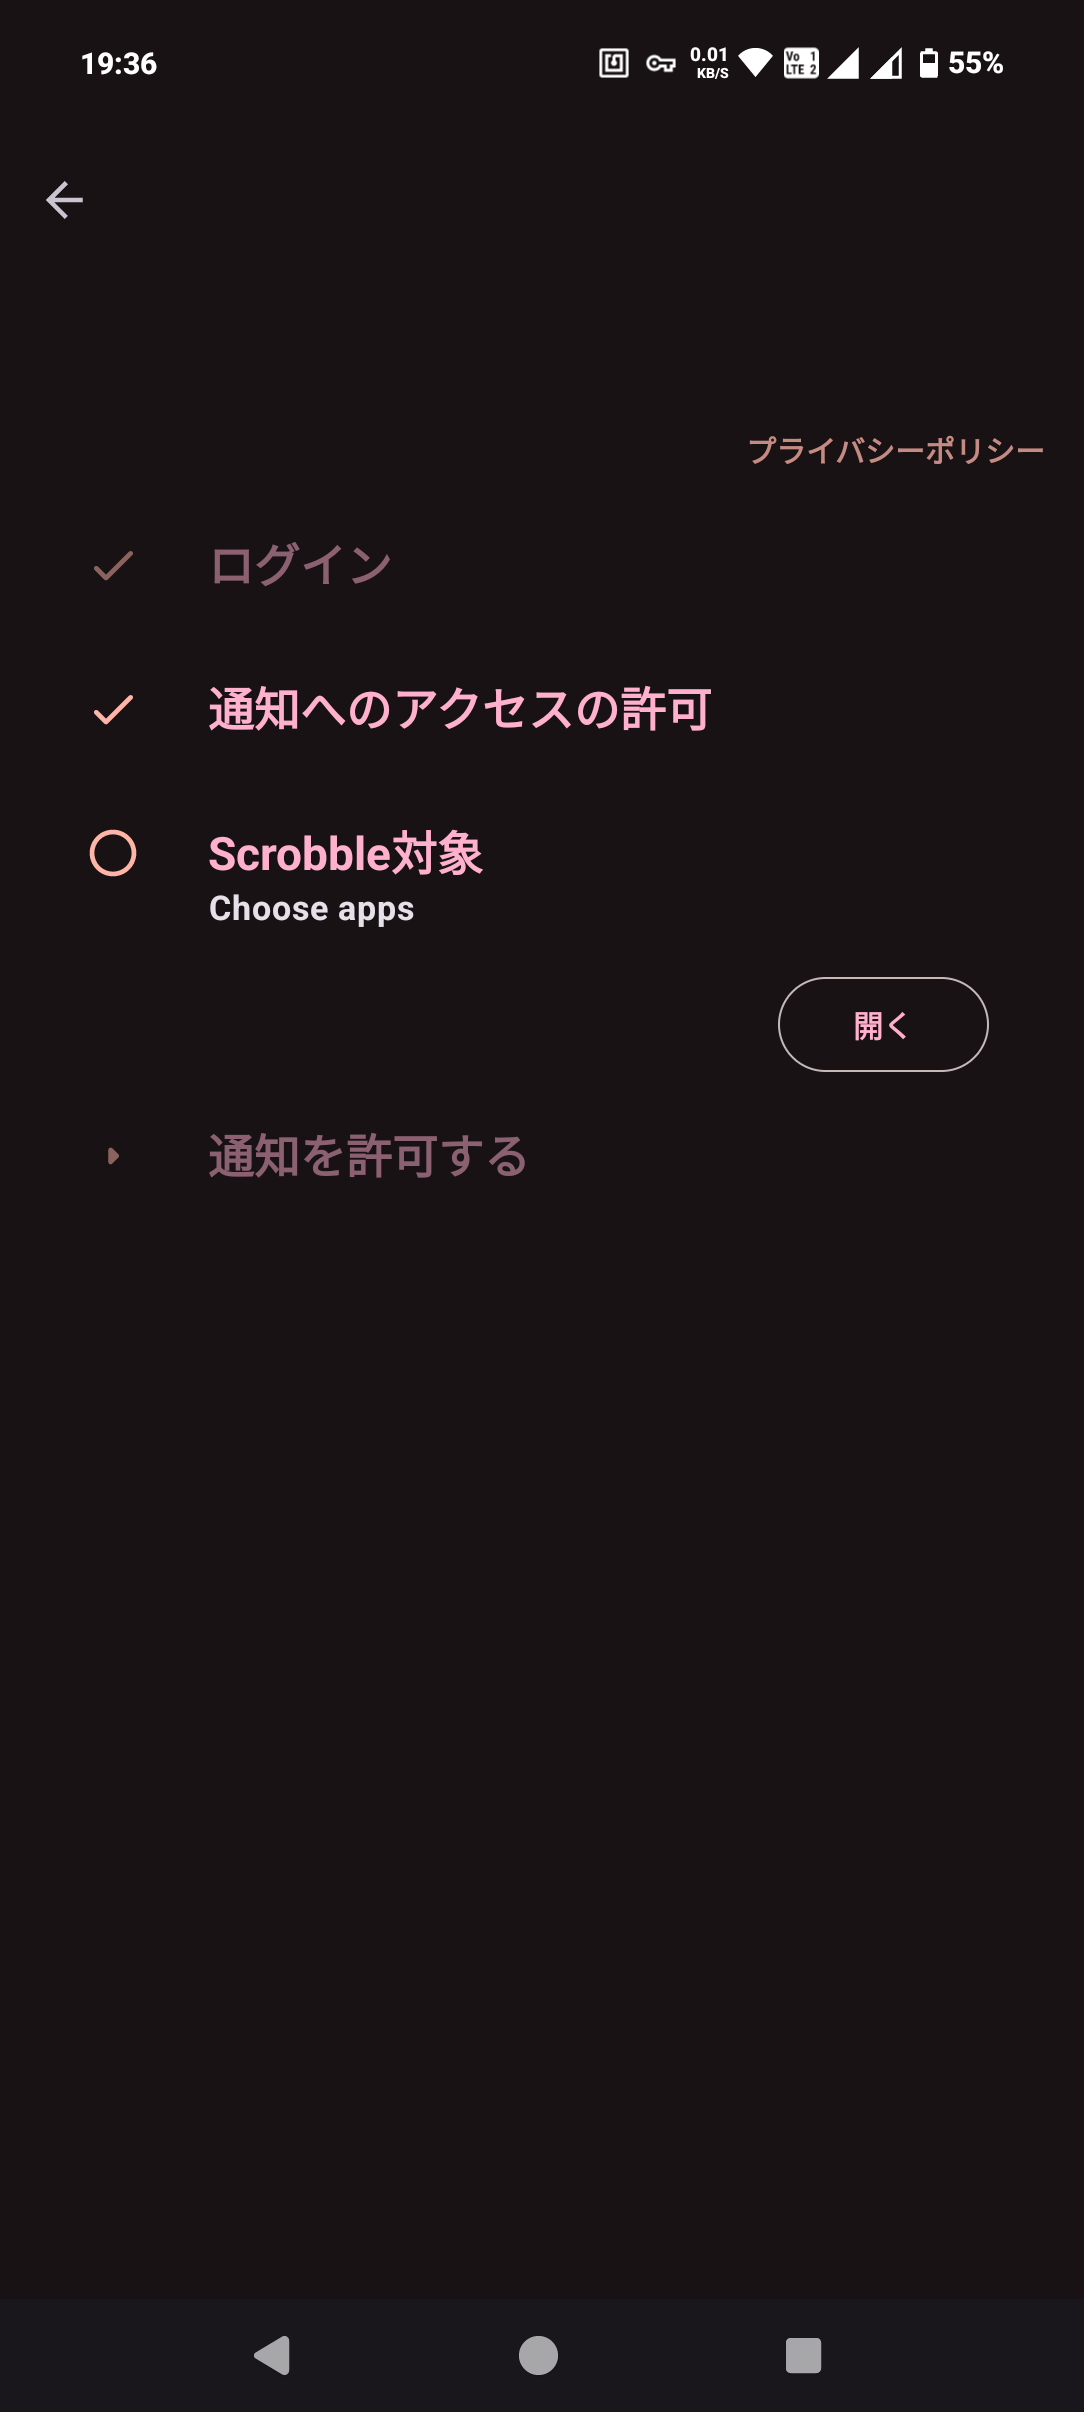
\includegraphics[width=5cm]{./pictures/lastfm8.png}
                        }
                        \label{img:lastfm8}
                    \end{minipage}
                    \begin{minipage}[b]{0.45\linewidth}
                        \centering
                        \fbox{
                            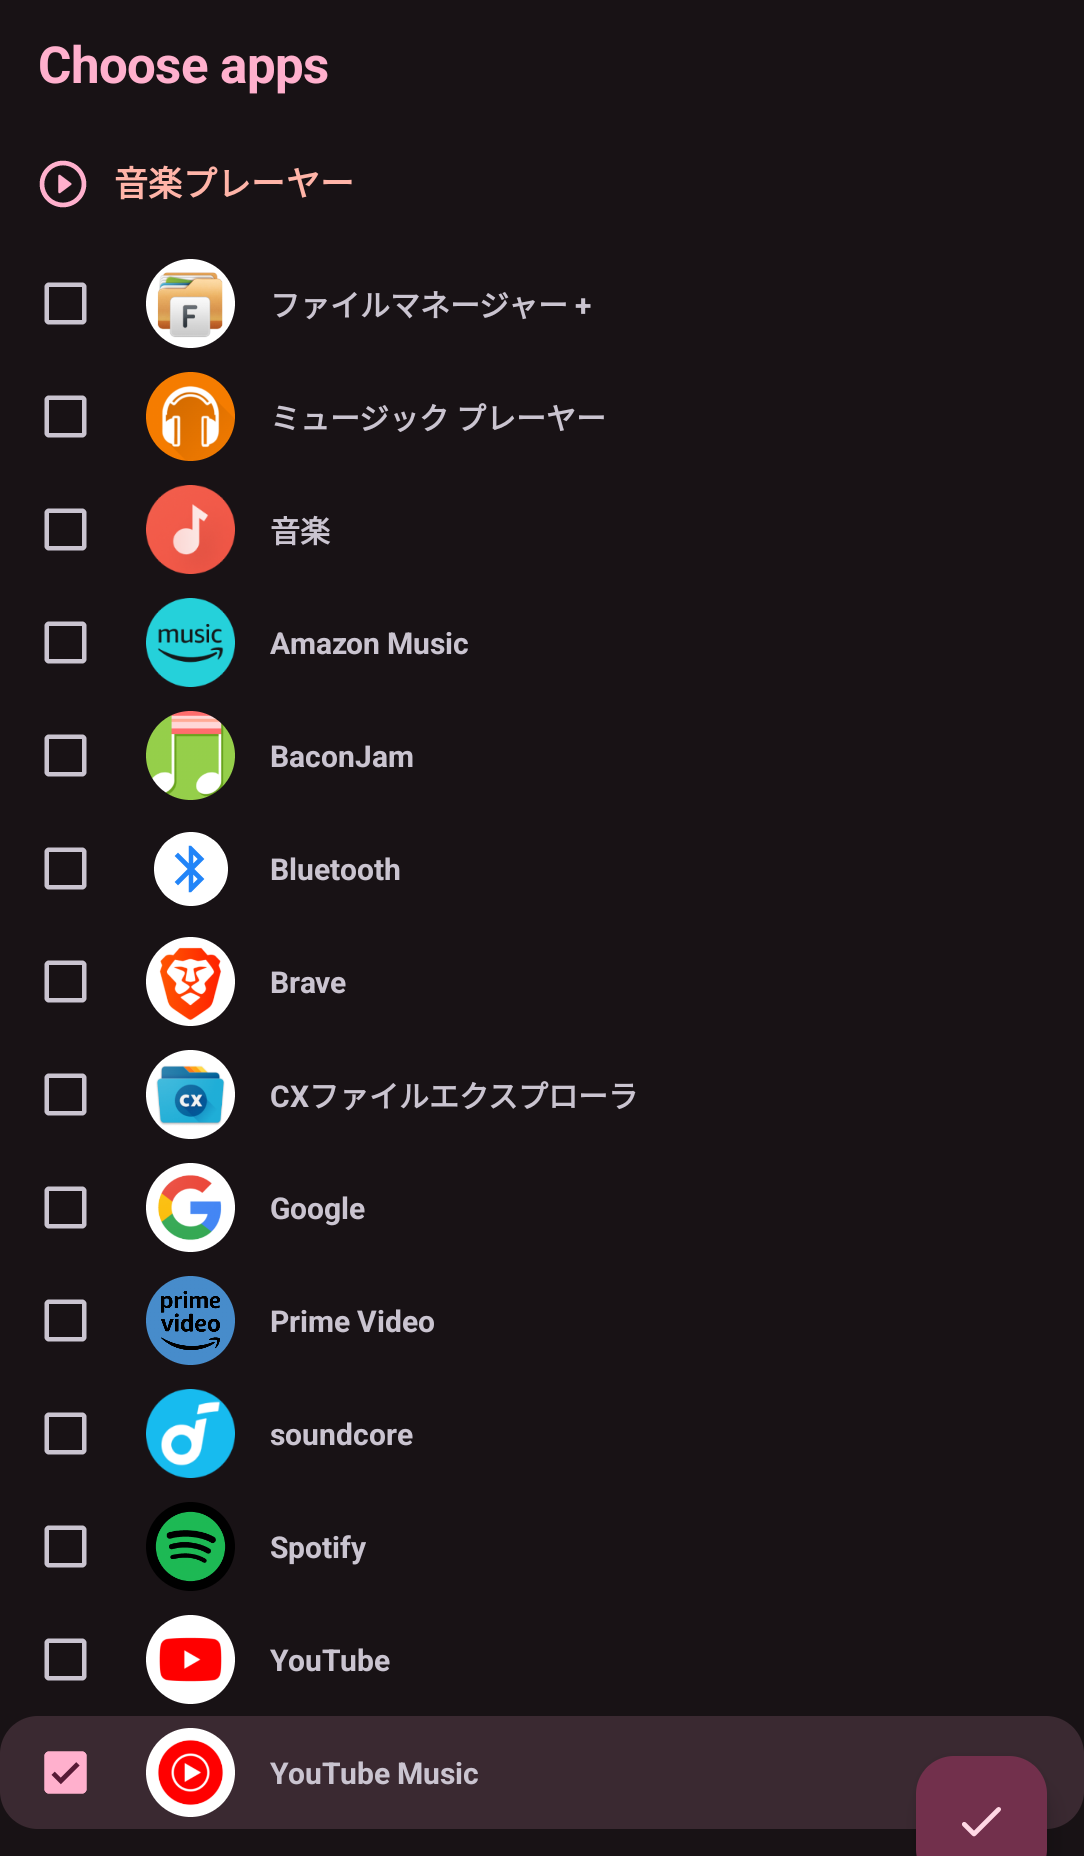
\includegraphics[width=5cm]{./pictures/lastfm9.png}
                        }
                        \label{img:lastfm9}
                    \end{minipage}
                    \caption*{対象アプリ選択}
                \end{figure}
            \item 通知を許可してください。

            \newpage
            \item アプリの設定を開き、「Scrobbleの遅延」の「分」を最小の30秒に設定したら、Pano Scrobblerの設定は完了です。
                \begin{figure}[htbp]
                    \centering
                    \fbox{
                        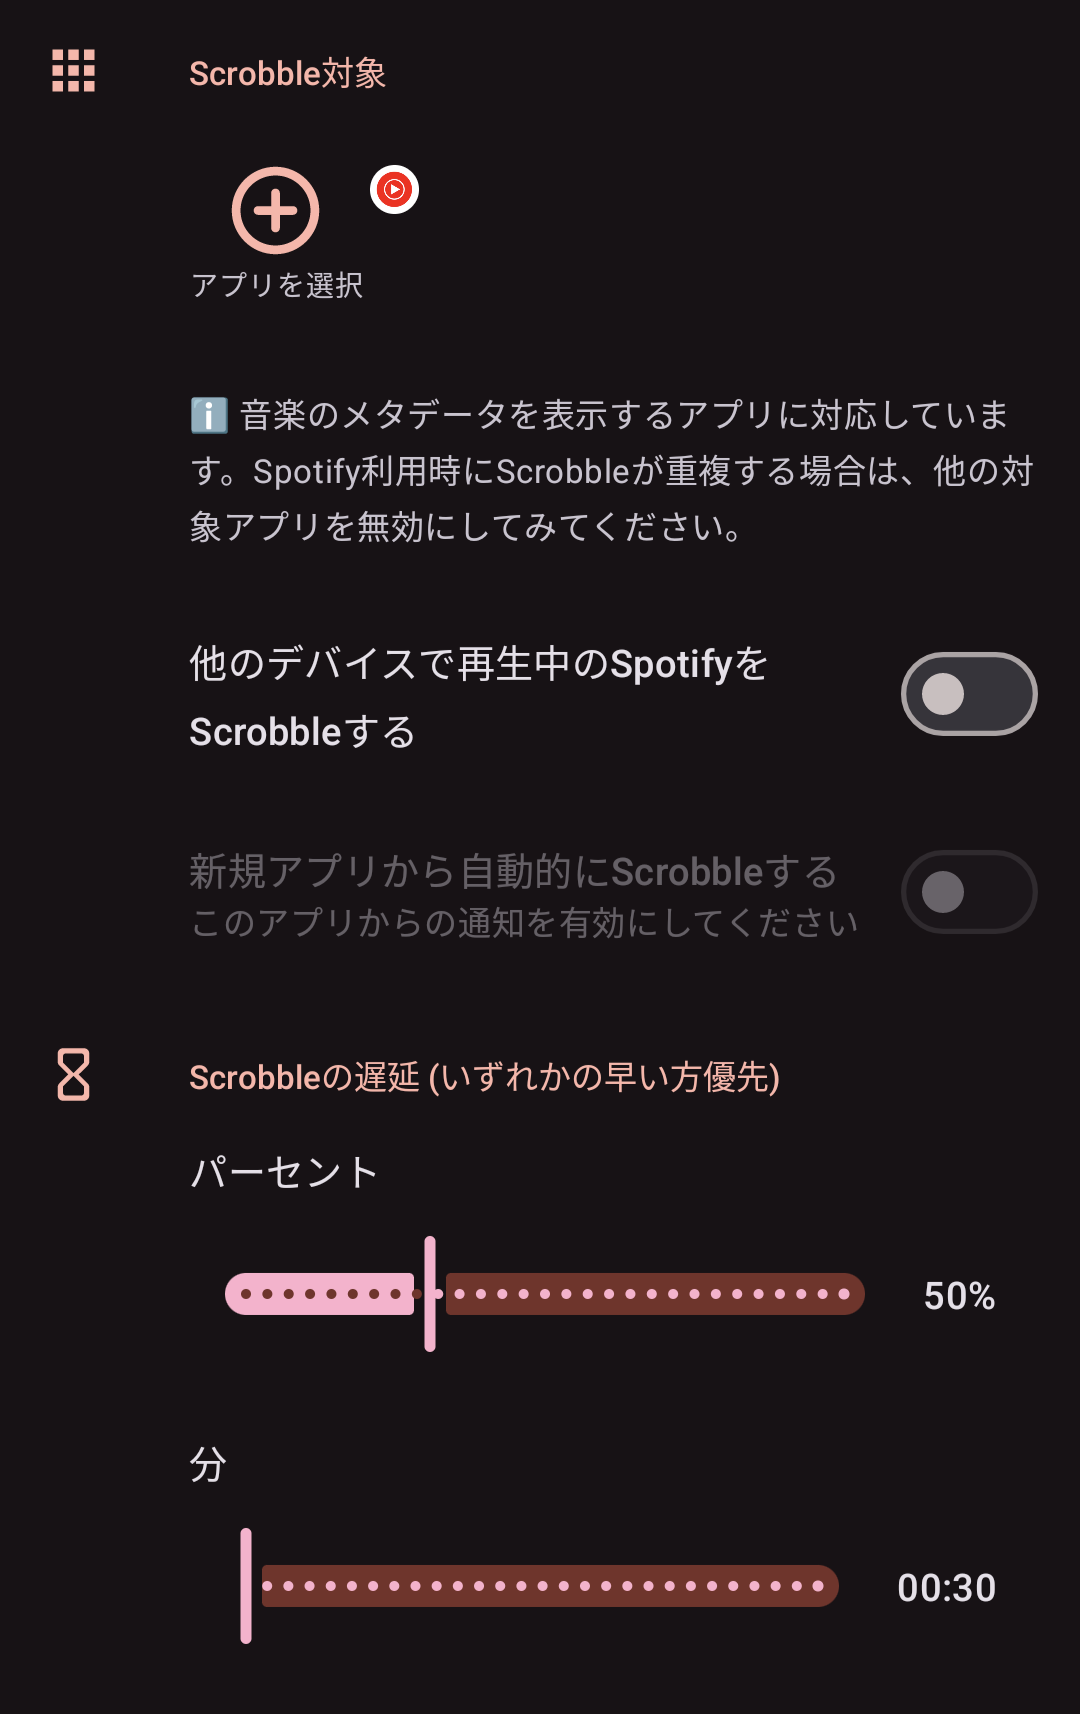
\includegraphics[width=6cm]{./pictures/lastfm10.png}
                    }
                    \caption{Scrobbleの遅延}
                    \label{img:lastfm10}
                \end{figure}
        \end{enumerate}

    \newpage
    \subsection{\bj 側の設定}
        \begin{enumerate}
            \item 設定画面の\ttbox{YouTube接続設定(プレビュー版)}を押下して、設定項目を展開してください。
                \begin{figure}[htbp]
                    \begin{minipage}[b]{0.45\linewidth}
                        \centering
                        \fbox{
                            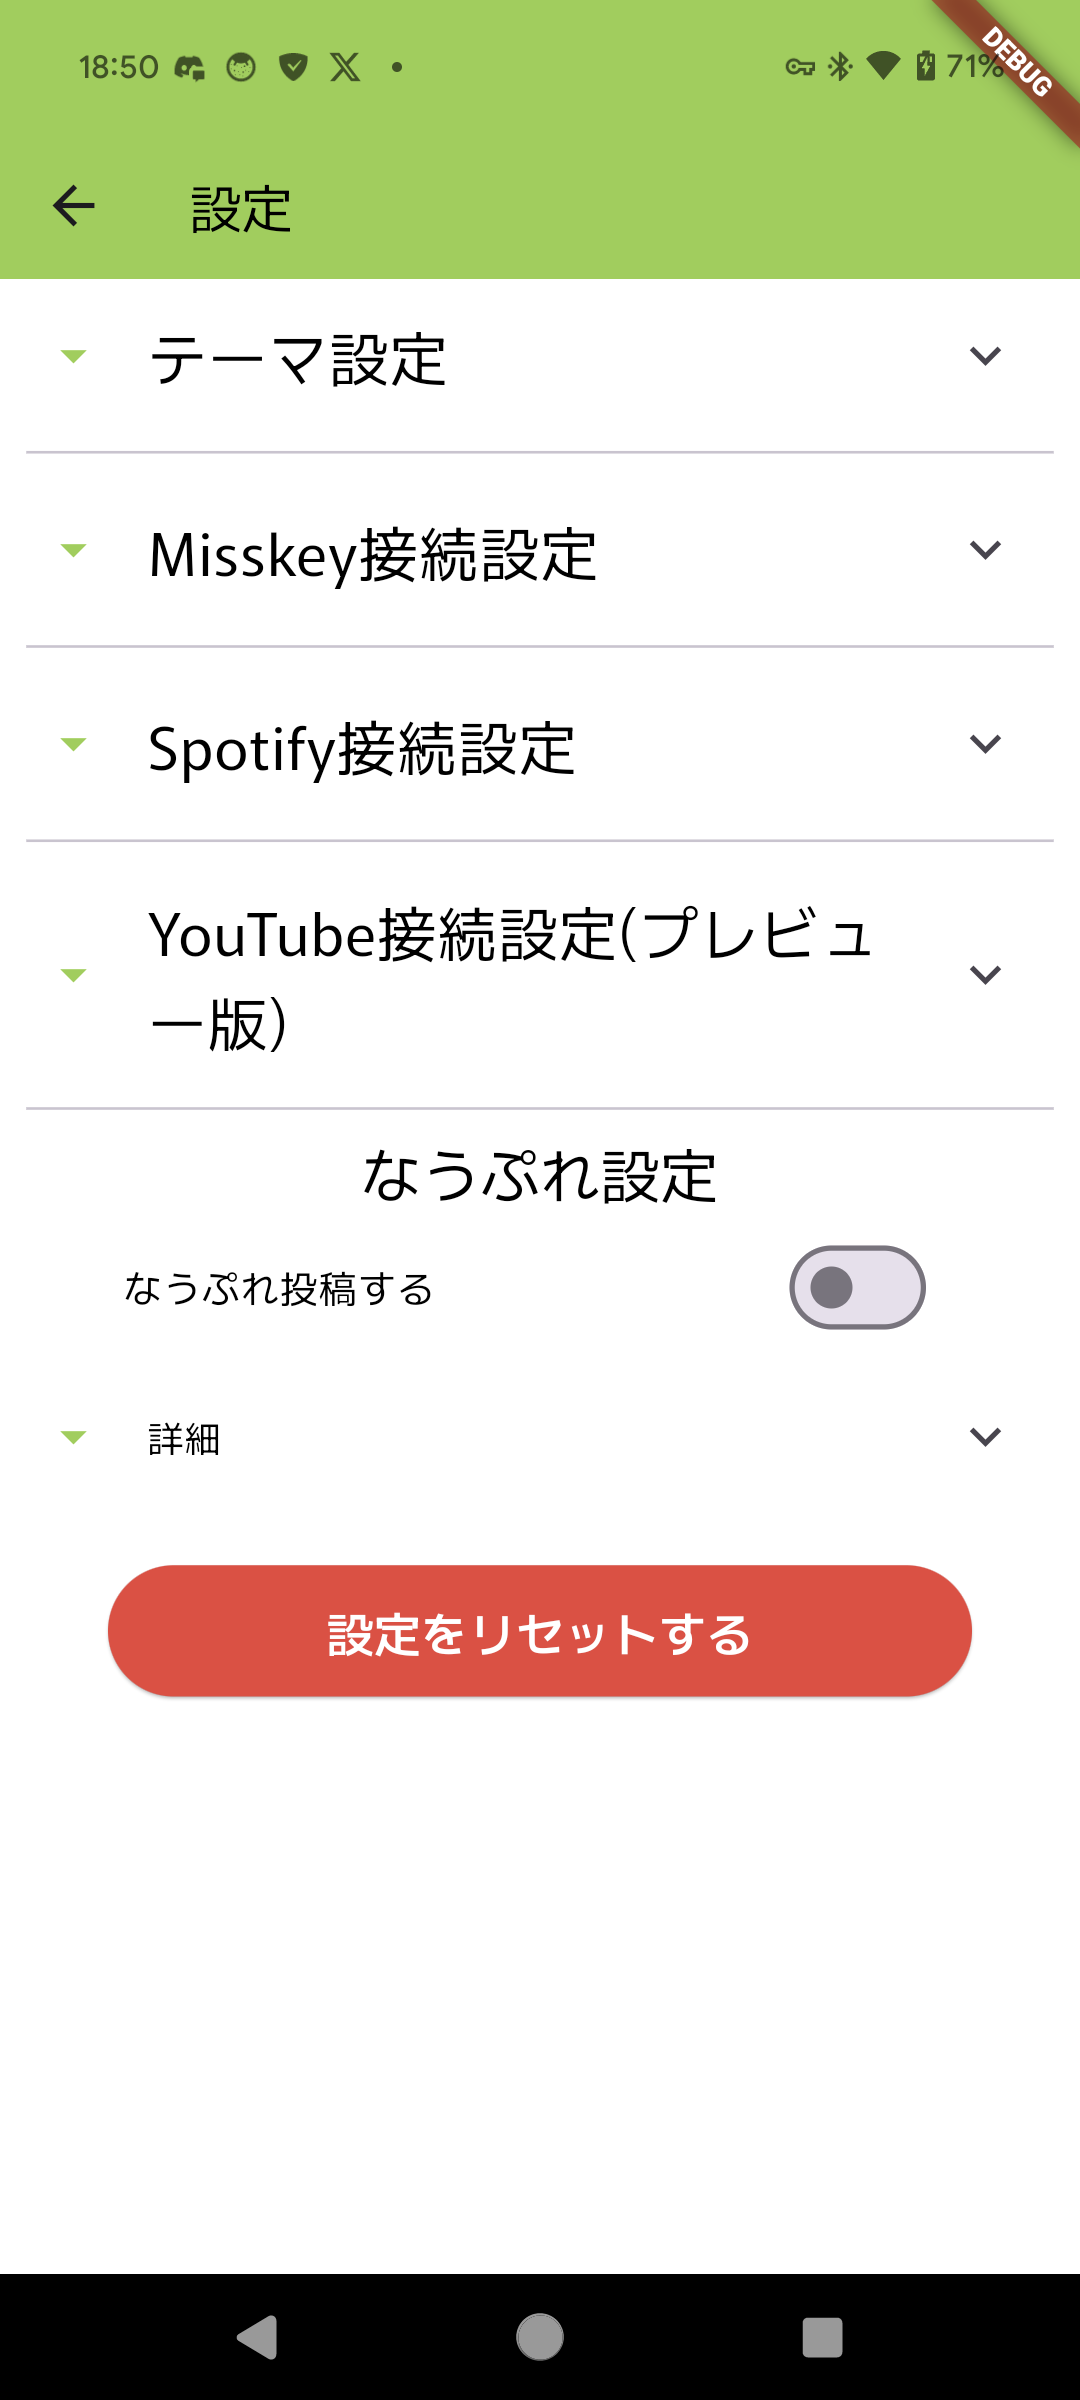
\includegraphics[width=5cm]{./pictures/lastfm11.png}
                        }
                        \caption{展開前}
                        \label{img:lastfm11}
                    \end{minipage}
                    \begin{minipage}[b]{0.45\linewidth}
                        \centering
                        \fbox{
                            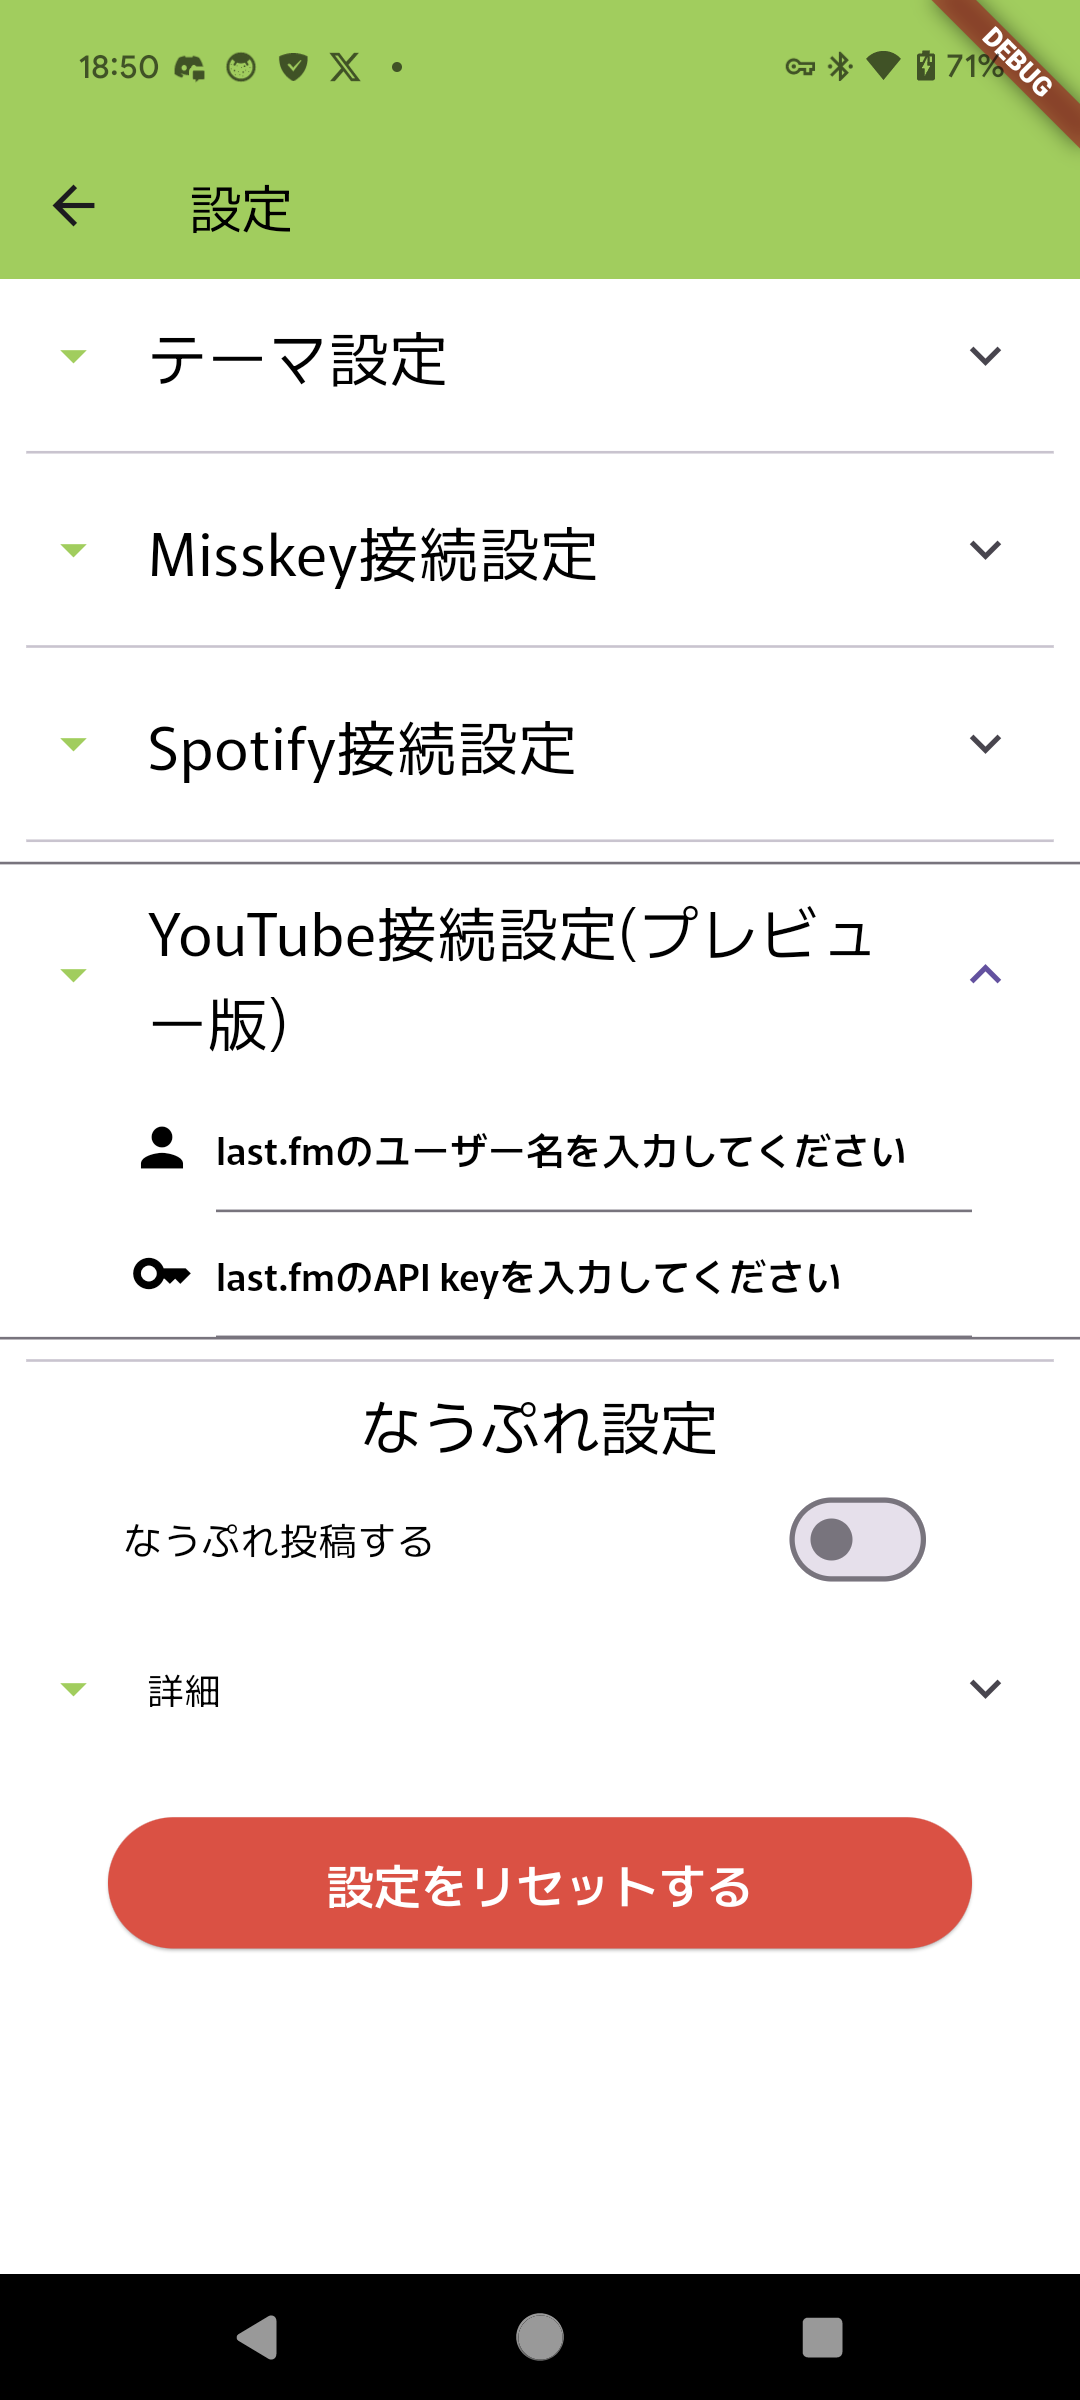
\includegraphics[width=5cm]{./pictures/lastfm12.png}
                        }
                        \caption{展開後}
                        \label{img:lastfm12}
                    \end{minipage}
                    \caption*{YouTube接続設定(プレビュー版)(\currentVersion)}
                \end{figure}

            \item \lastfm のユーザー名と、先ほど控えた\texttt{API key}を入力してください。
        \end{enumerate}

\newpage
\section{操作説明}
    \subsection{投稿範囲の設定}
    \begin{enumerate}
        \item 設定画面の\ttbox{なうぷれ設定}→\ttbox{詳細}を押下して展開してください。
            \begin{figure}[htbp]
                \begin{minipage}[b]{0.45\linewidth}
                    \centering
                    \fbox{
                        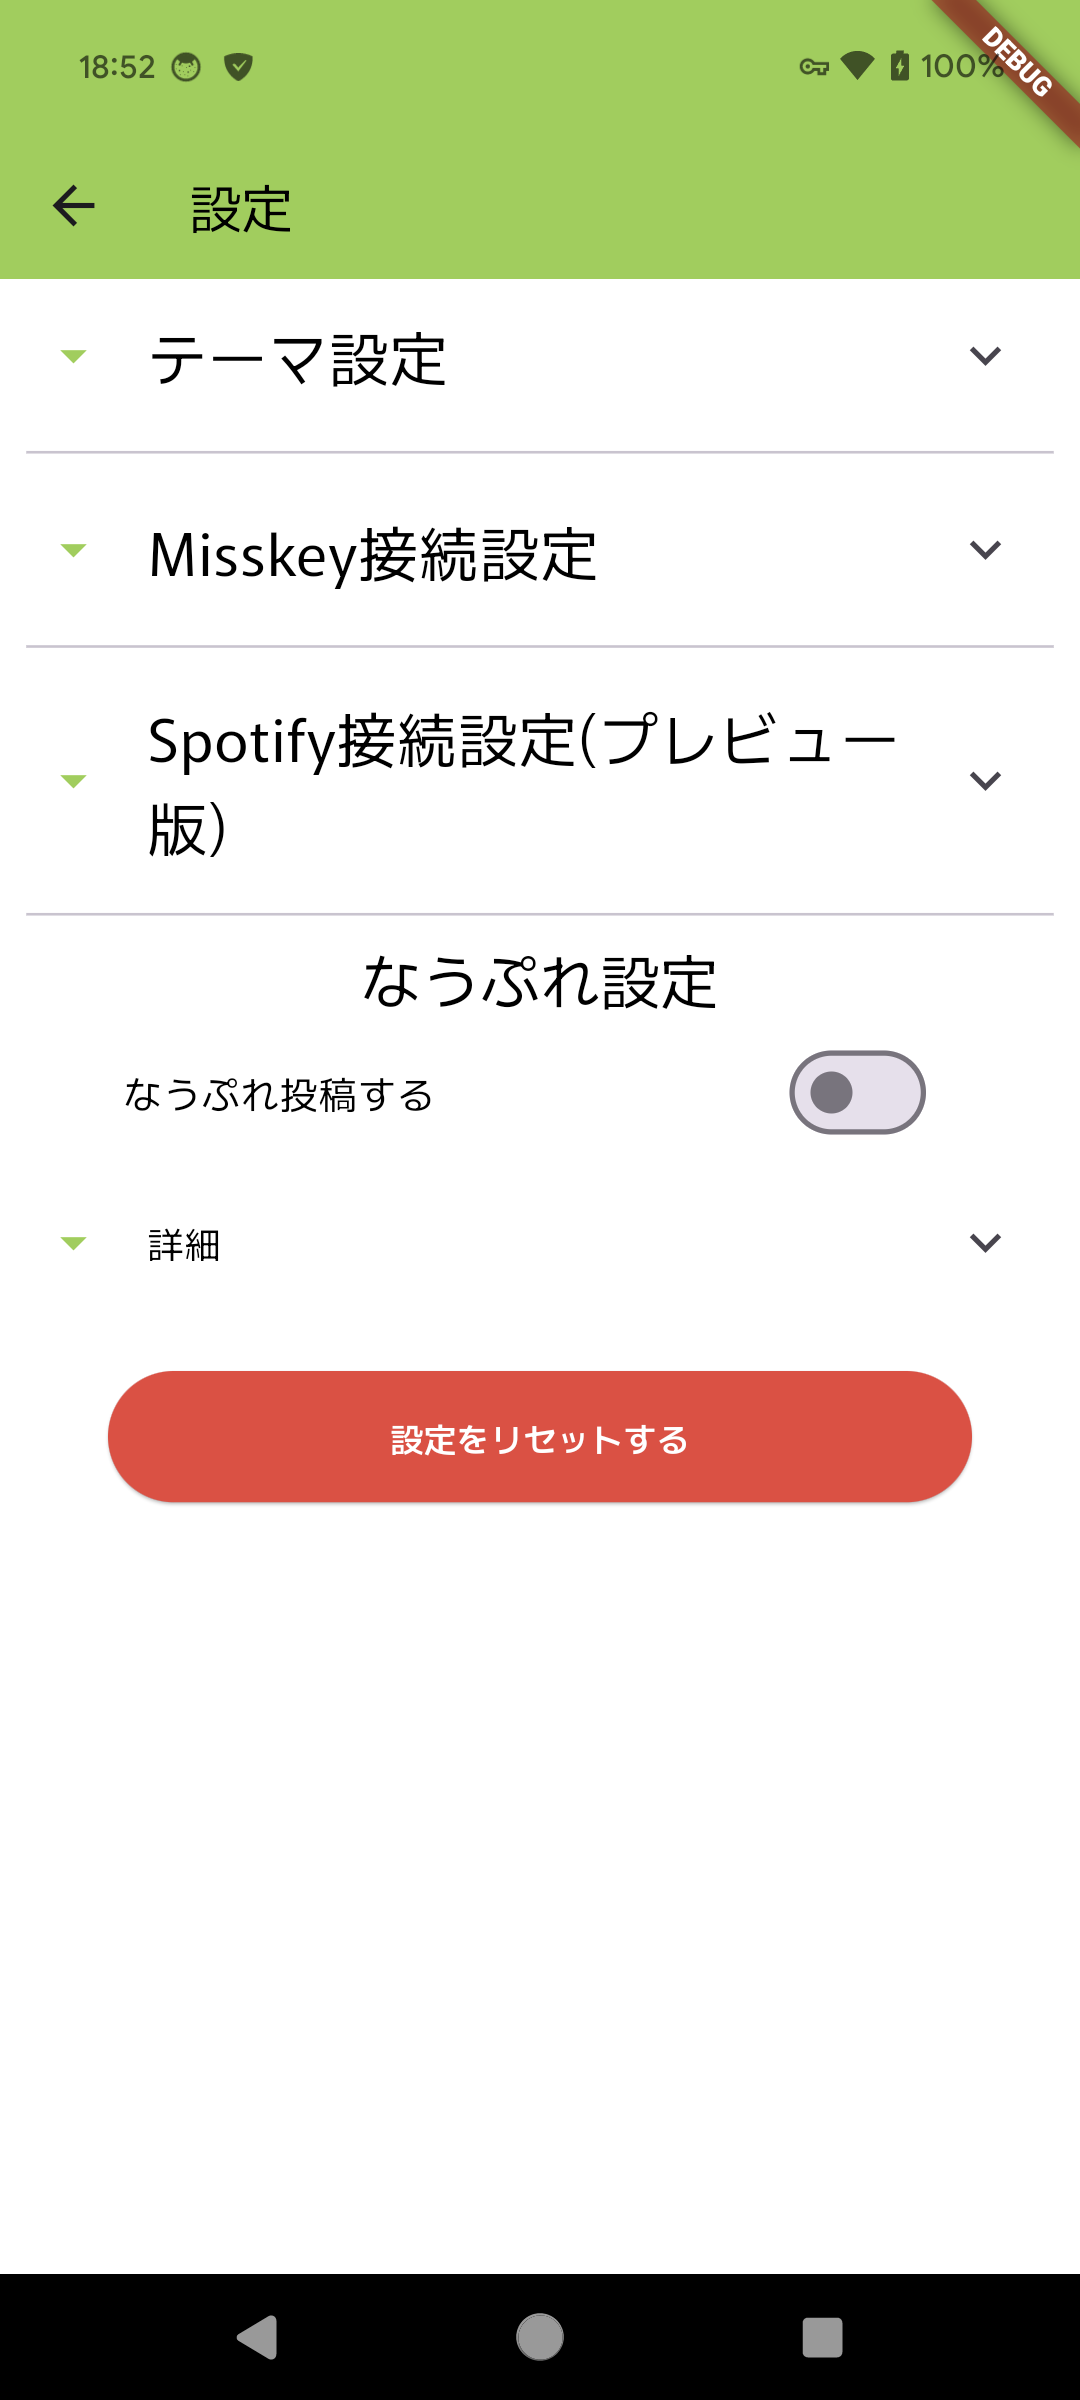
\includegraphics[width=5cm]{./pictures/guide1.png}
                    }
                    \caption{展開前}
                    \label{img:guide1}
                \end{minipage}
                \begin{minipage}[b]{0.45\linewidth}
                    \centering
                    \fbox{
                        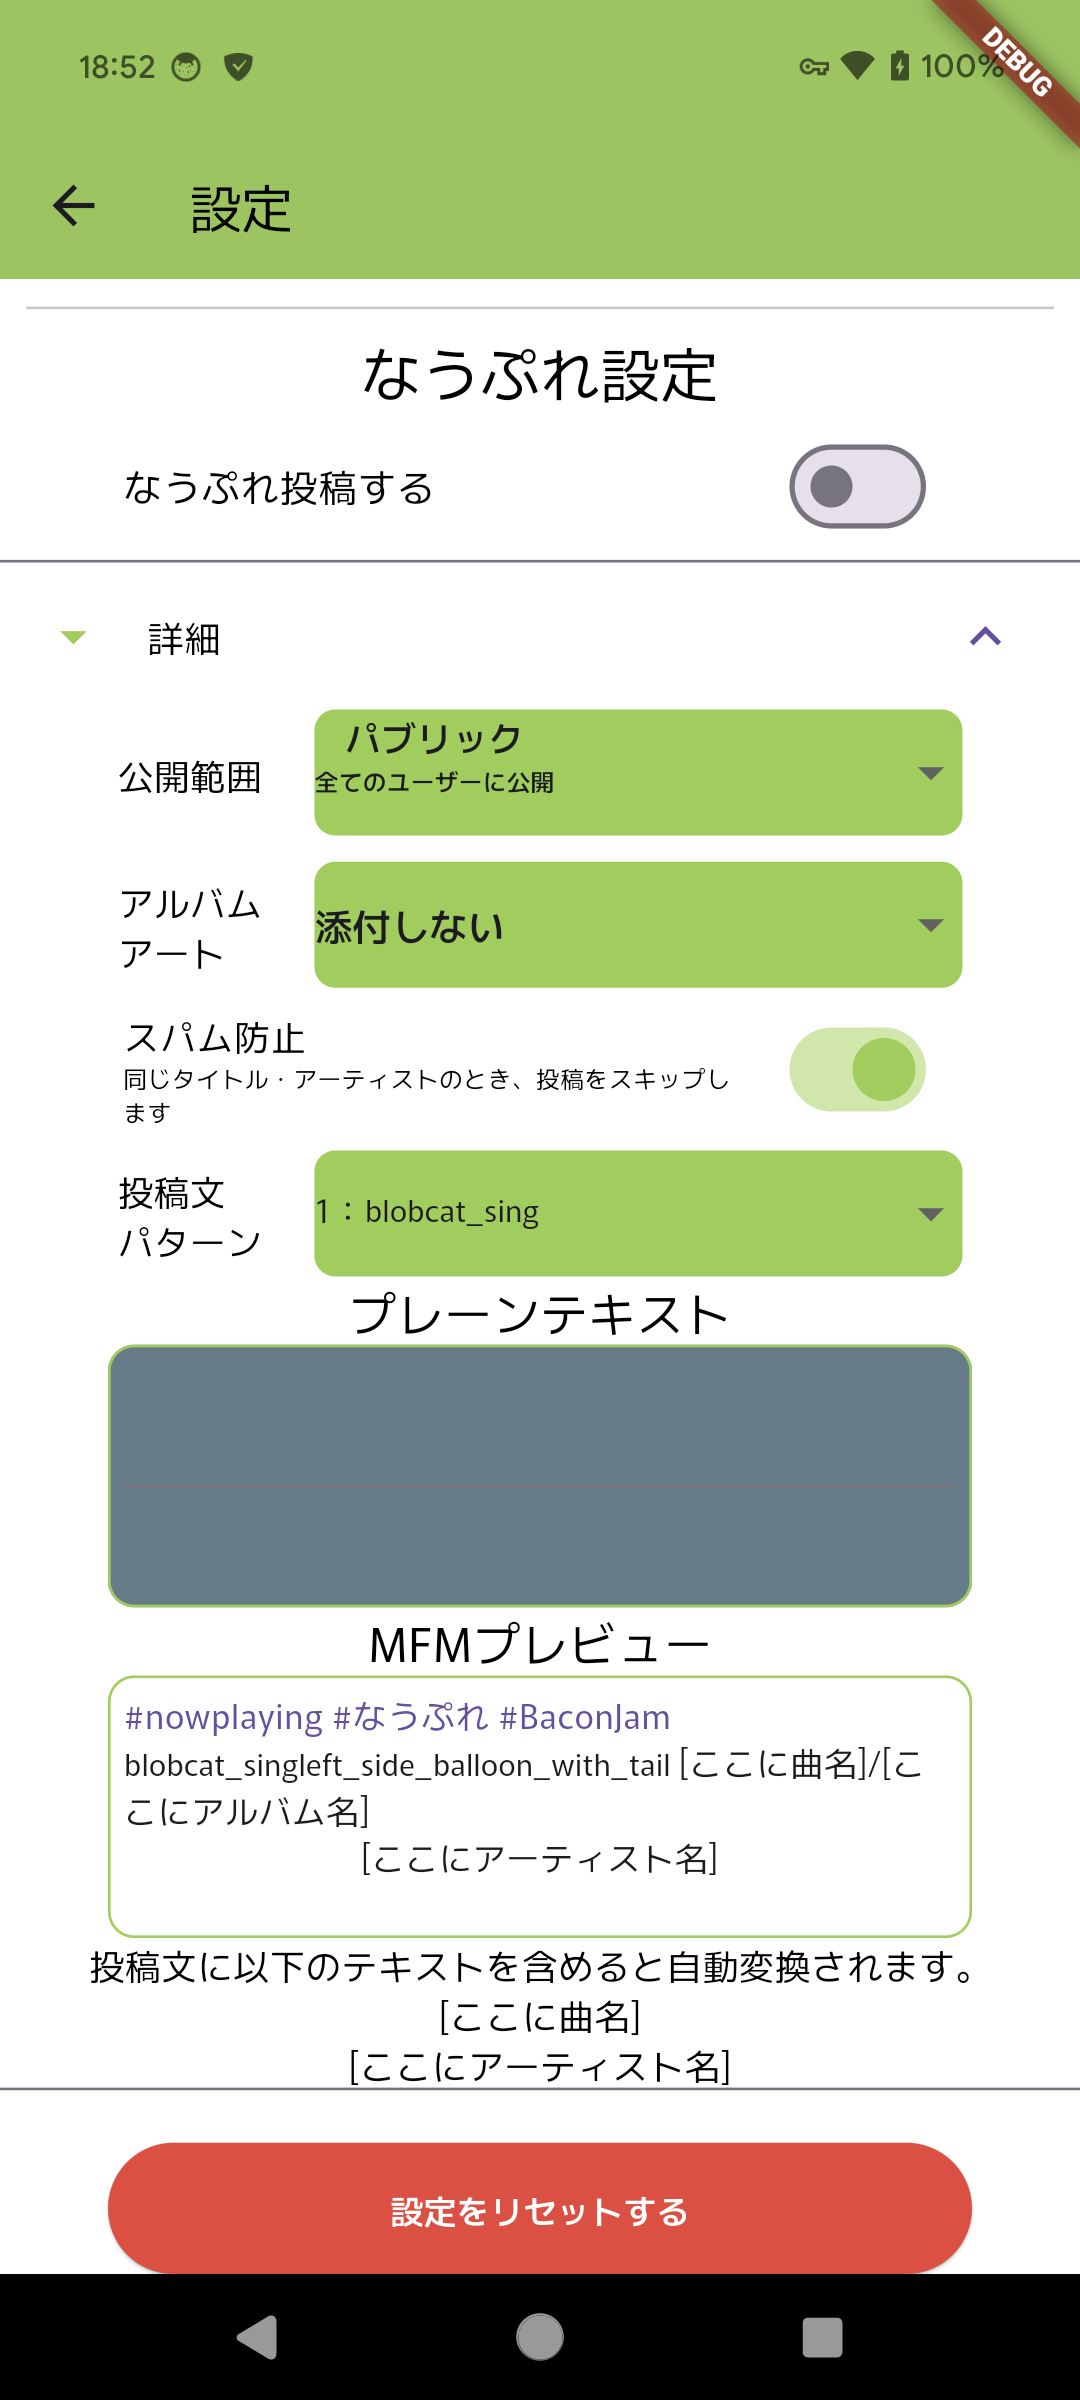
\includegraphics[width=5cm]{./pictures/guide2.png}
                    }
                    \caption{展開後}
                    \label{img:guide2}
                \end{minipage}
                \caption*{\mi なうぷれ設定の詳細(\currentVersion)}
            \end{figure}

        \newpage
        \item 公開範囲のドロップダウンで\ttbox{チャンネル}を選択して、\ttbox{チャンネルを選択}を押下してください。
            \begin{figure}[htbp]
                \begin{minipage}[b]{0.45\linewidth}
                    \centering
                    \fbox{
                        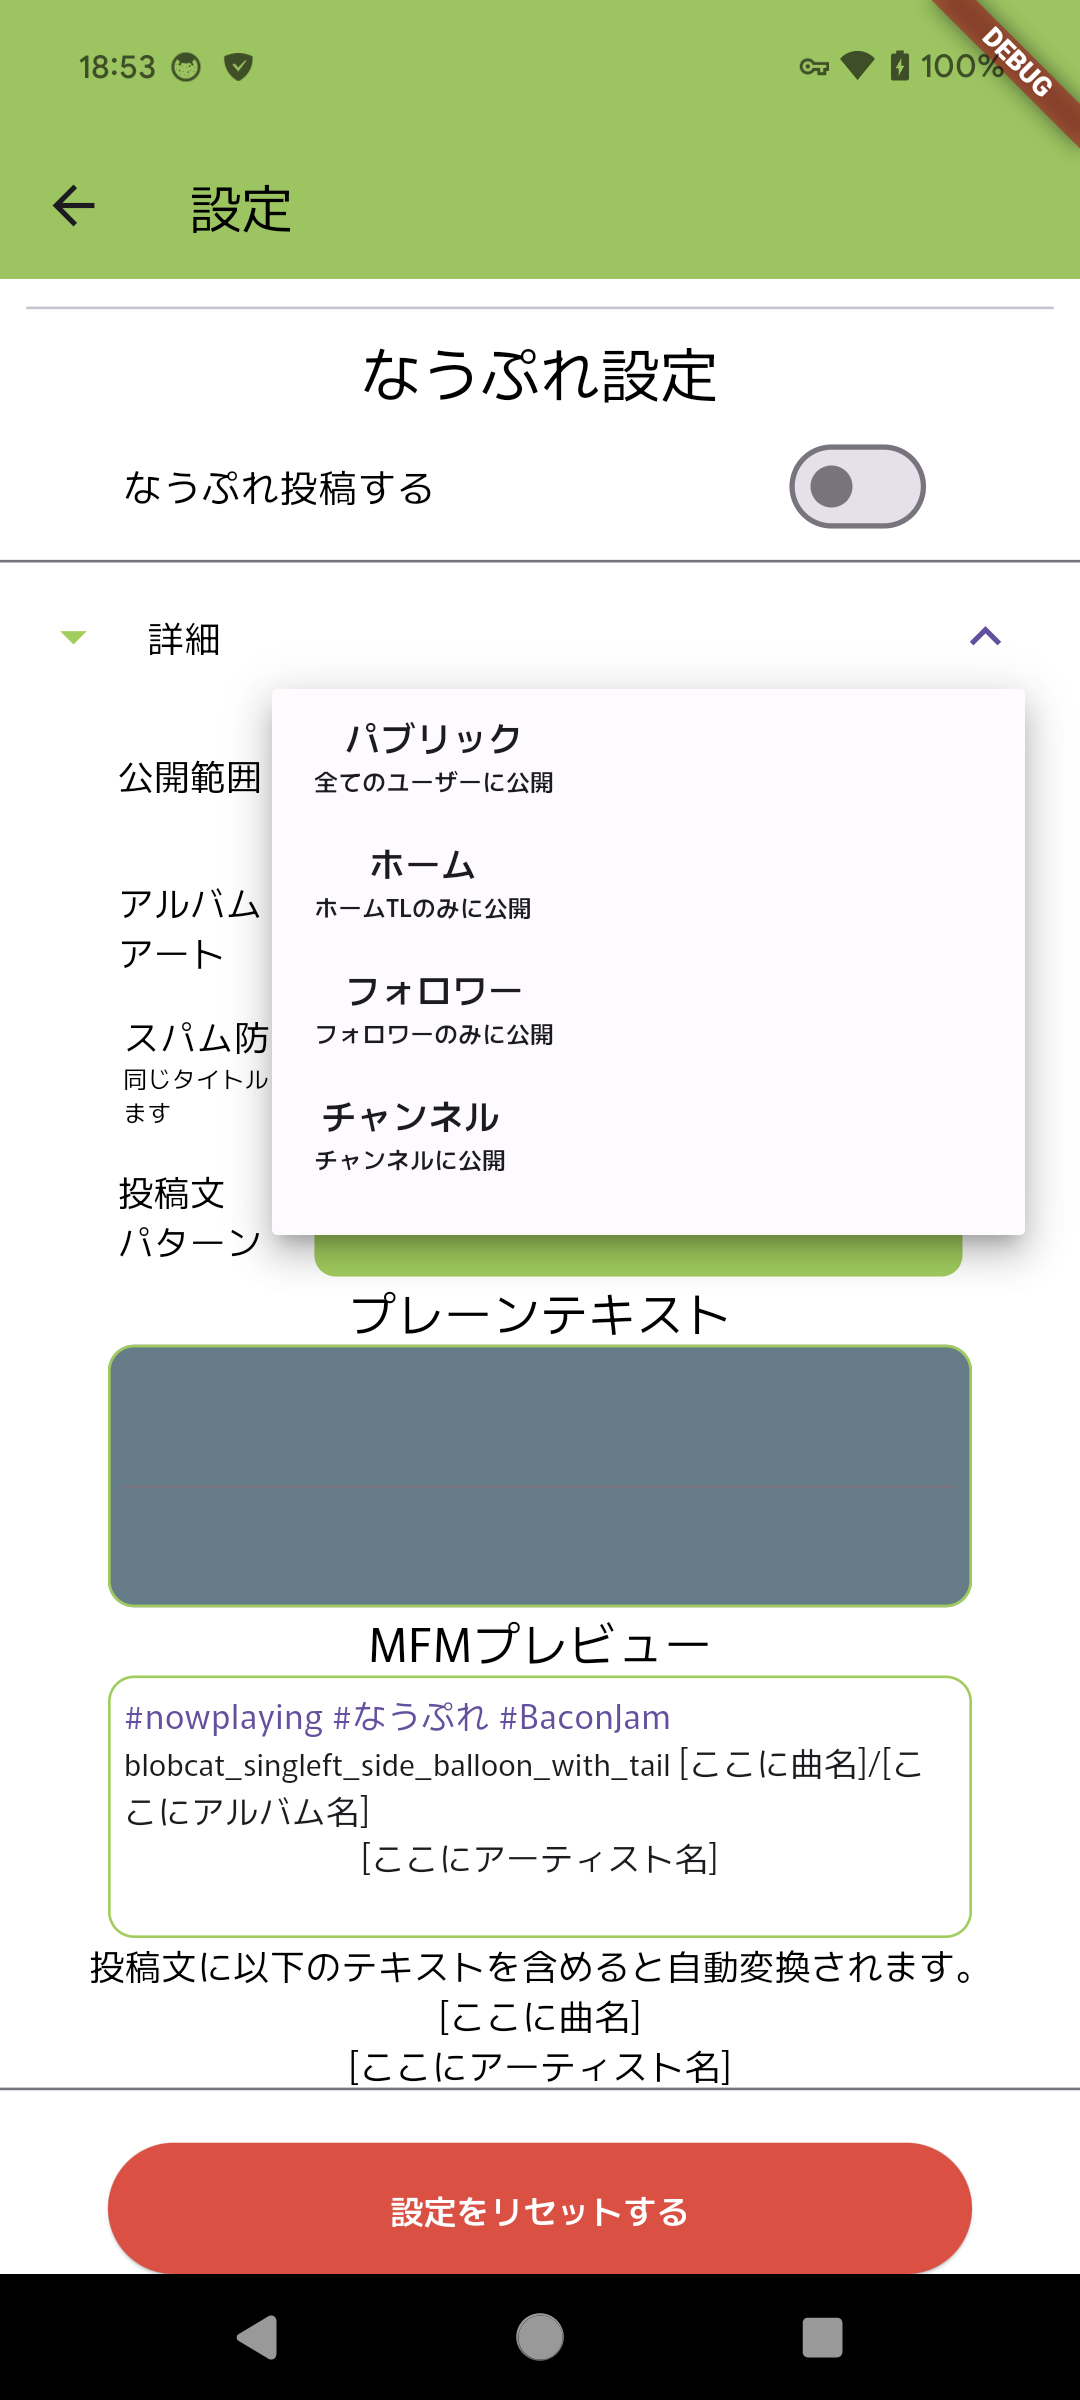
\includegraphics[width=5cm]{./pictures/guide3.png}
                    }
                    \caption{ドロップダウン一覧}
                    \label{img:guide3}
                \end{minipage}
                \begin{minipage}[b]{0.45\linewidth}
                    \centering
                    \fbox{
                        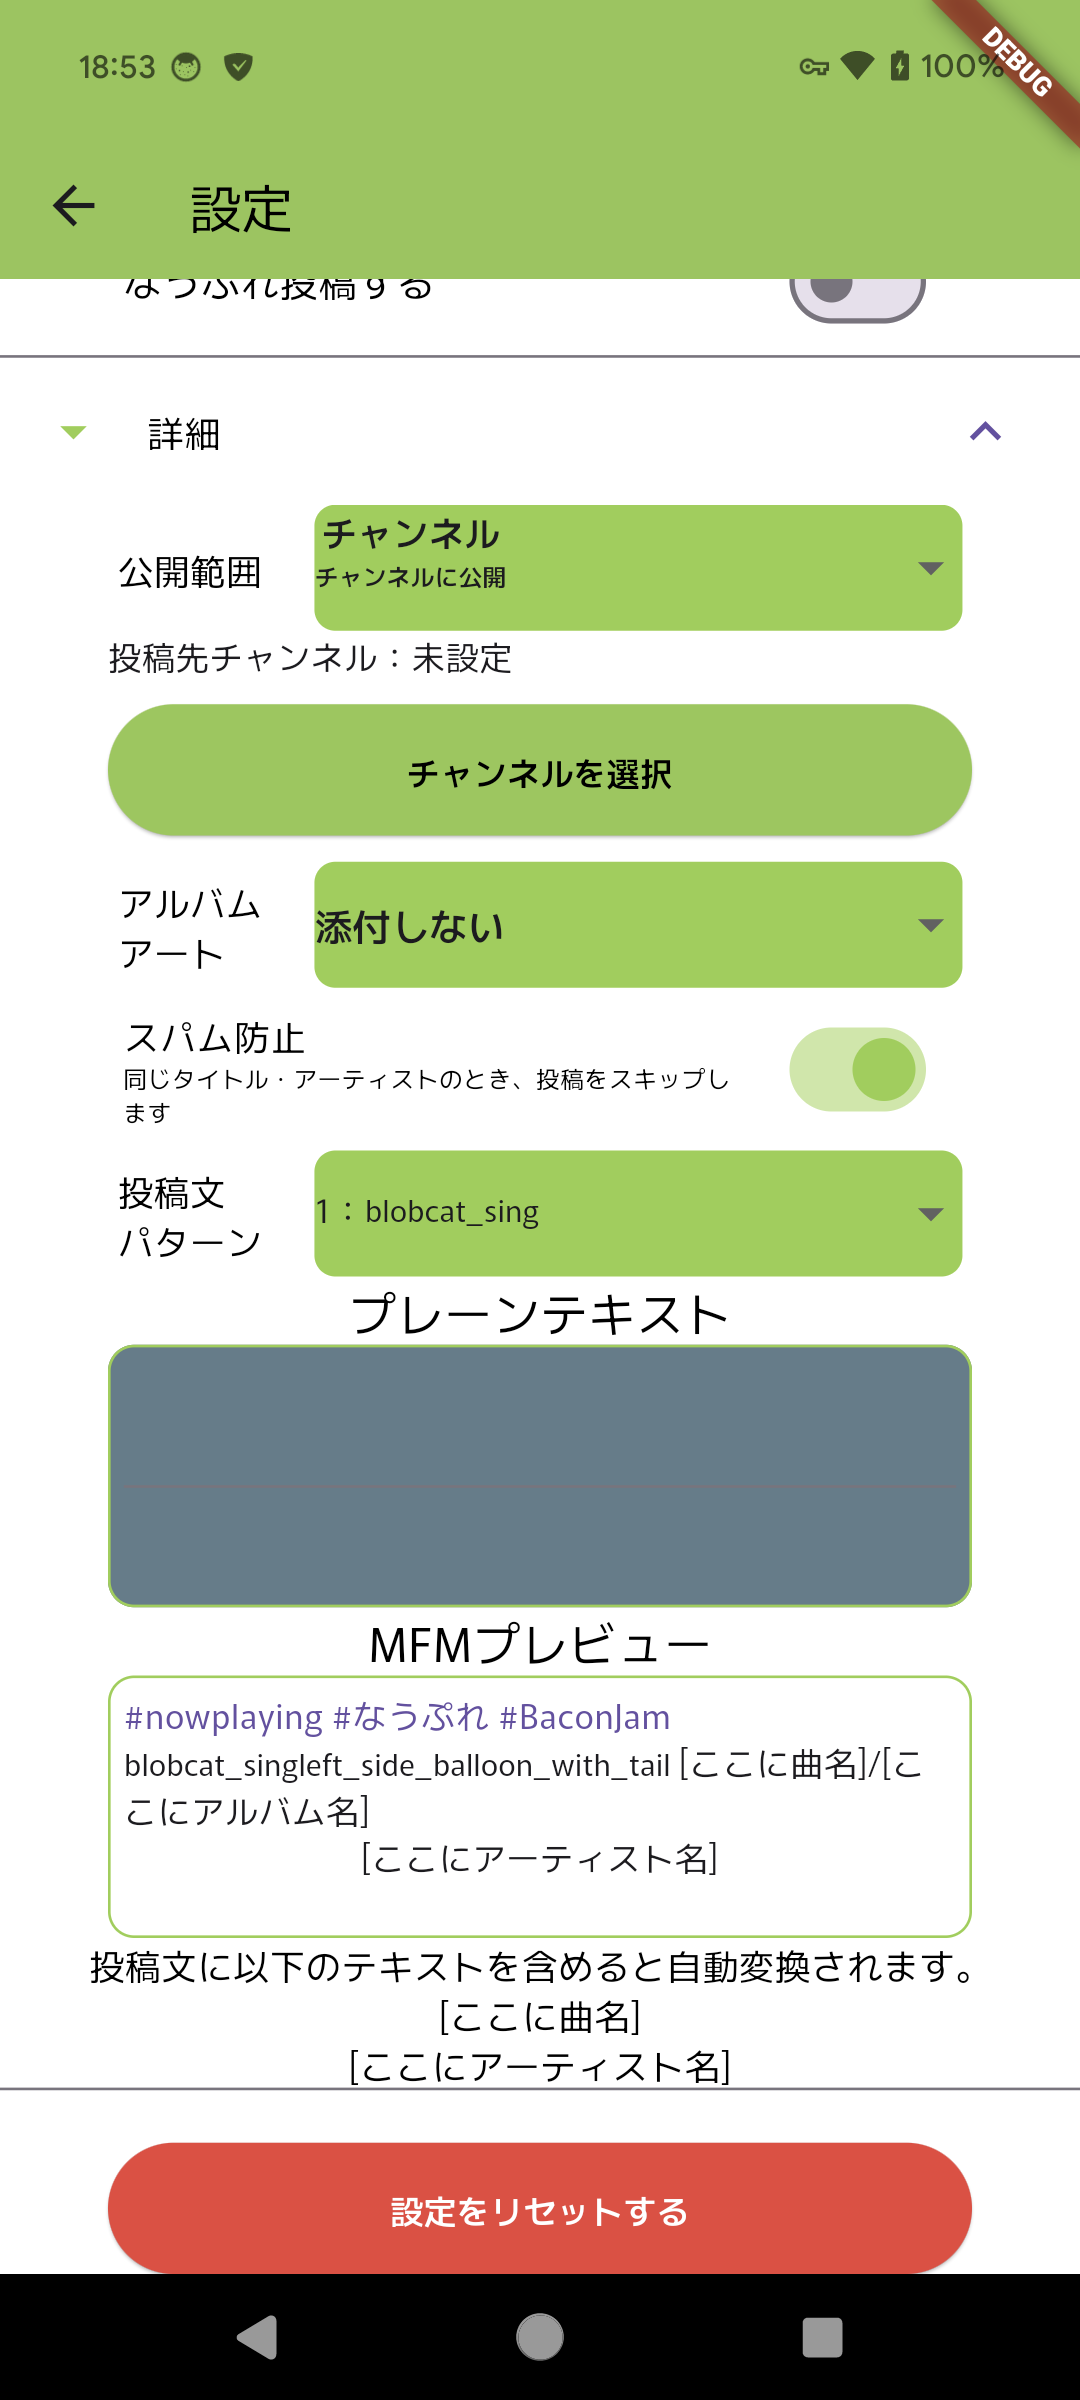
\includegraphics[width=5cm]{./pictures/guide4.png}
                    }
                    \caption{チャンネルを選択した場合}
                    \label{img:guide4}
                \end{minipage}
                \caption*{\mi 公開範囲の選択(\currentVersion)}
            \end{figure}

        \newpage
        \item チャンネル検索ページで、チャンネルの名称を入力して検索してください。
            \begin{figure}[htbp]
                \centering
                \fbox{
                    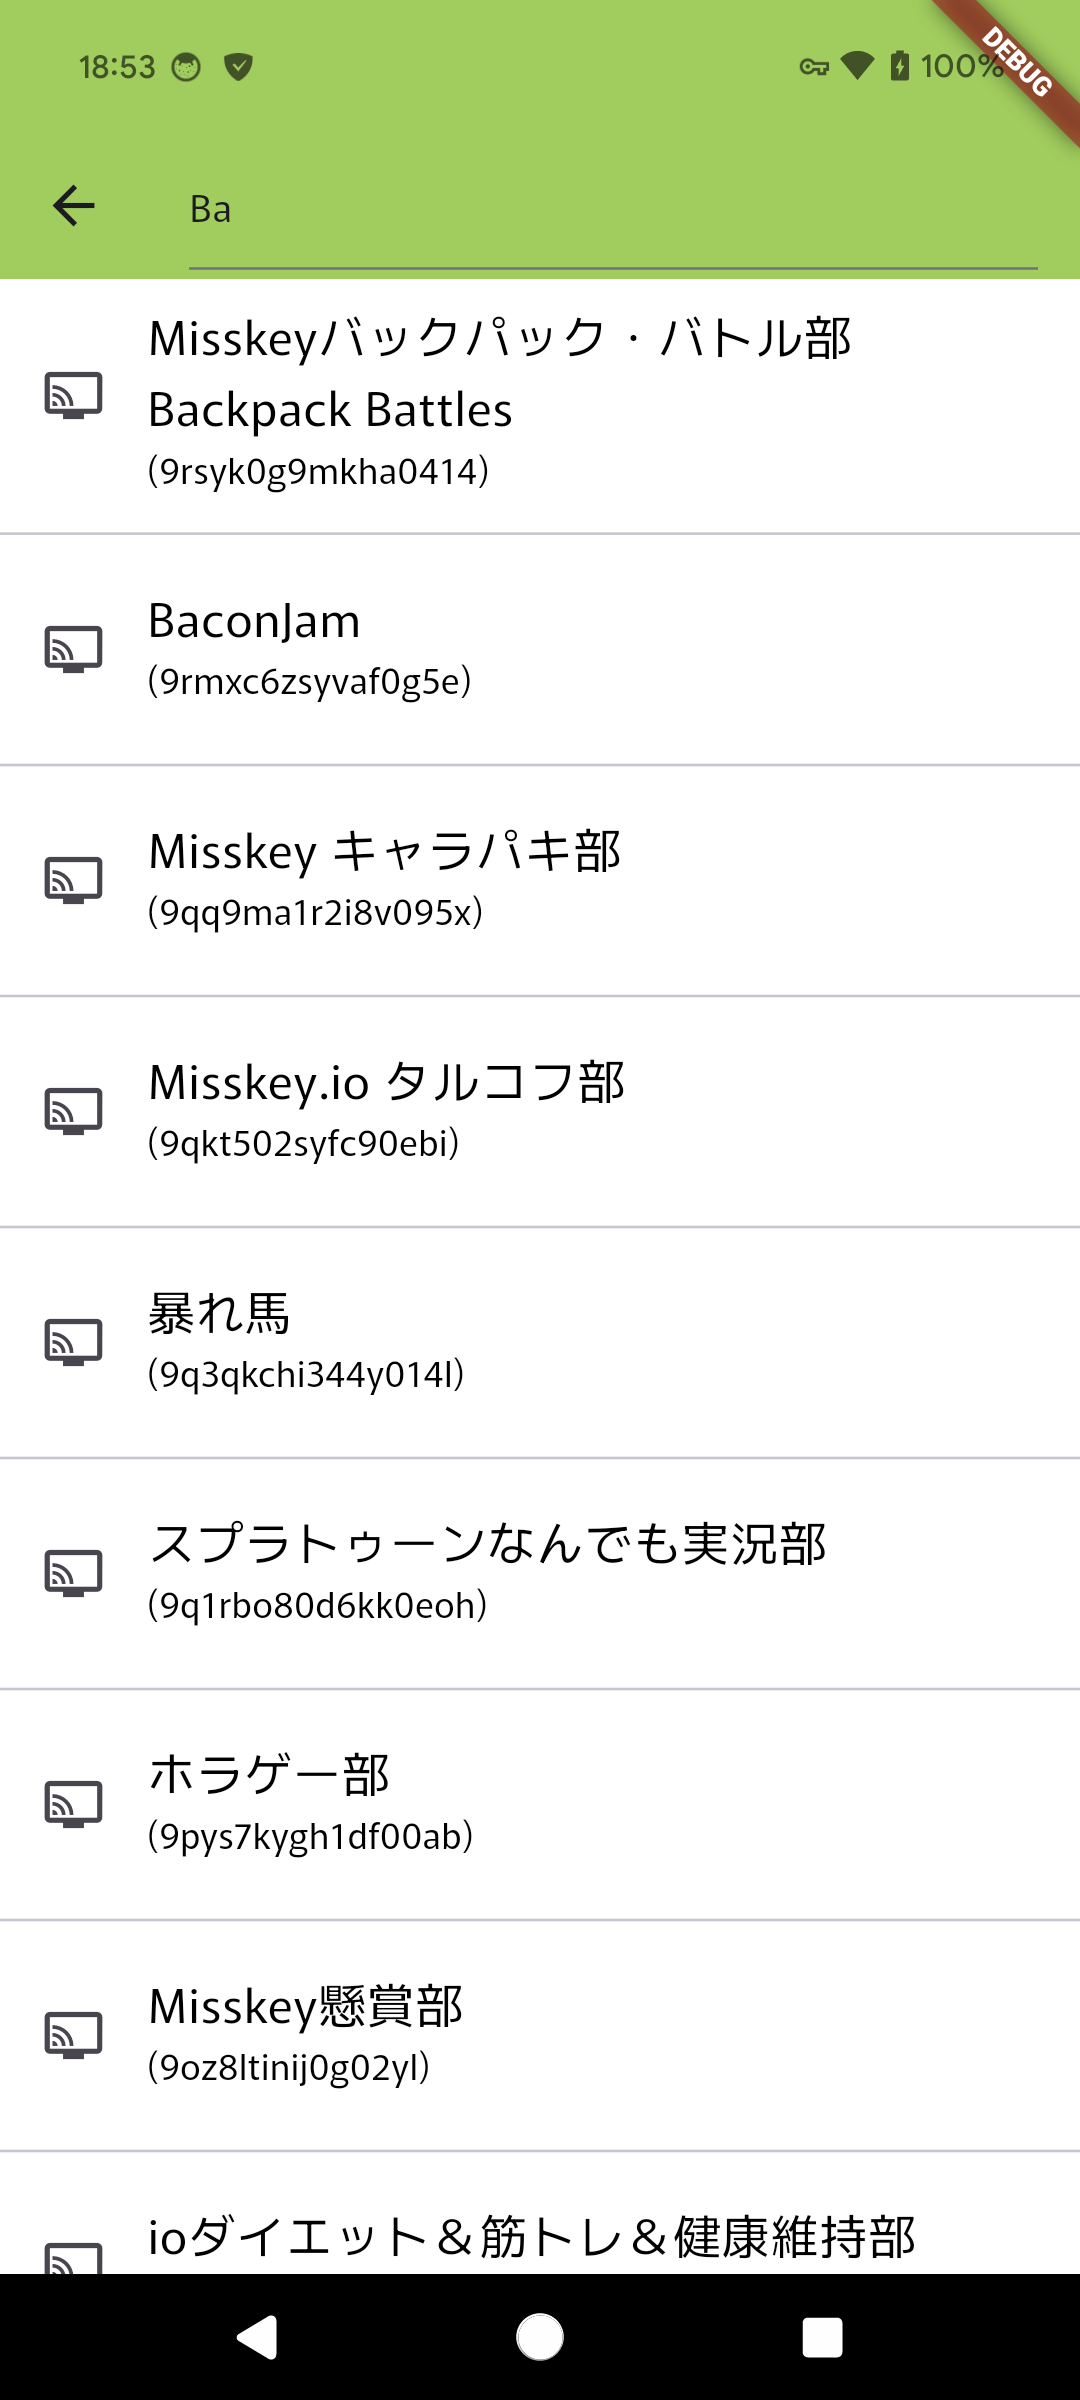
\includegraphics[width=5cm]{./pictures/guide5.png}
                }
                \caption{チャンネル検索ページ(\currentVersion)}
                \label{img:guide5}
            \end{figure}

        \newpage
        \item 投稿したいチャンネル名を押下すると、そのチャンネルを指定して設定画面に戻ります。
            \begin{figure}[htbp]
                \centering
                \fbox{
                    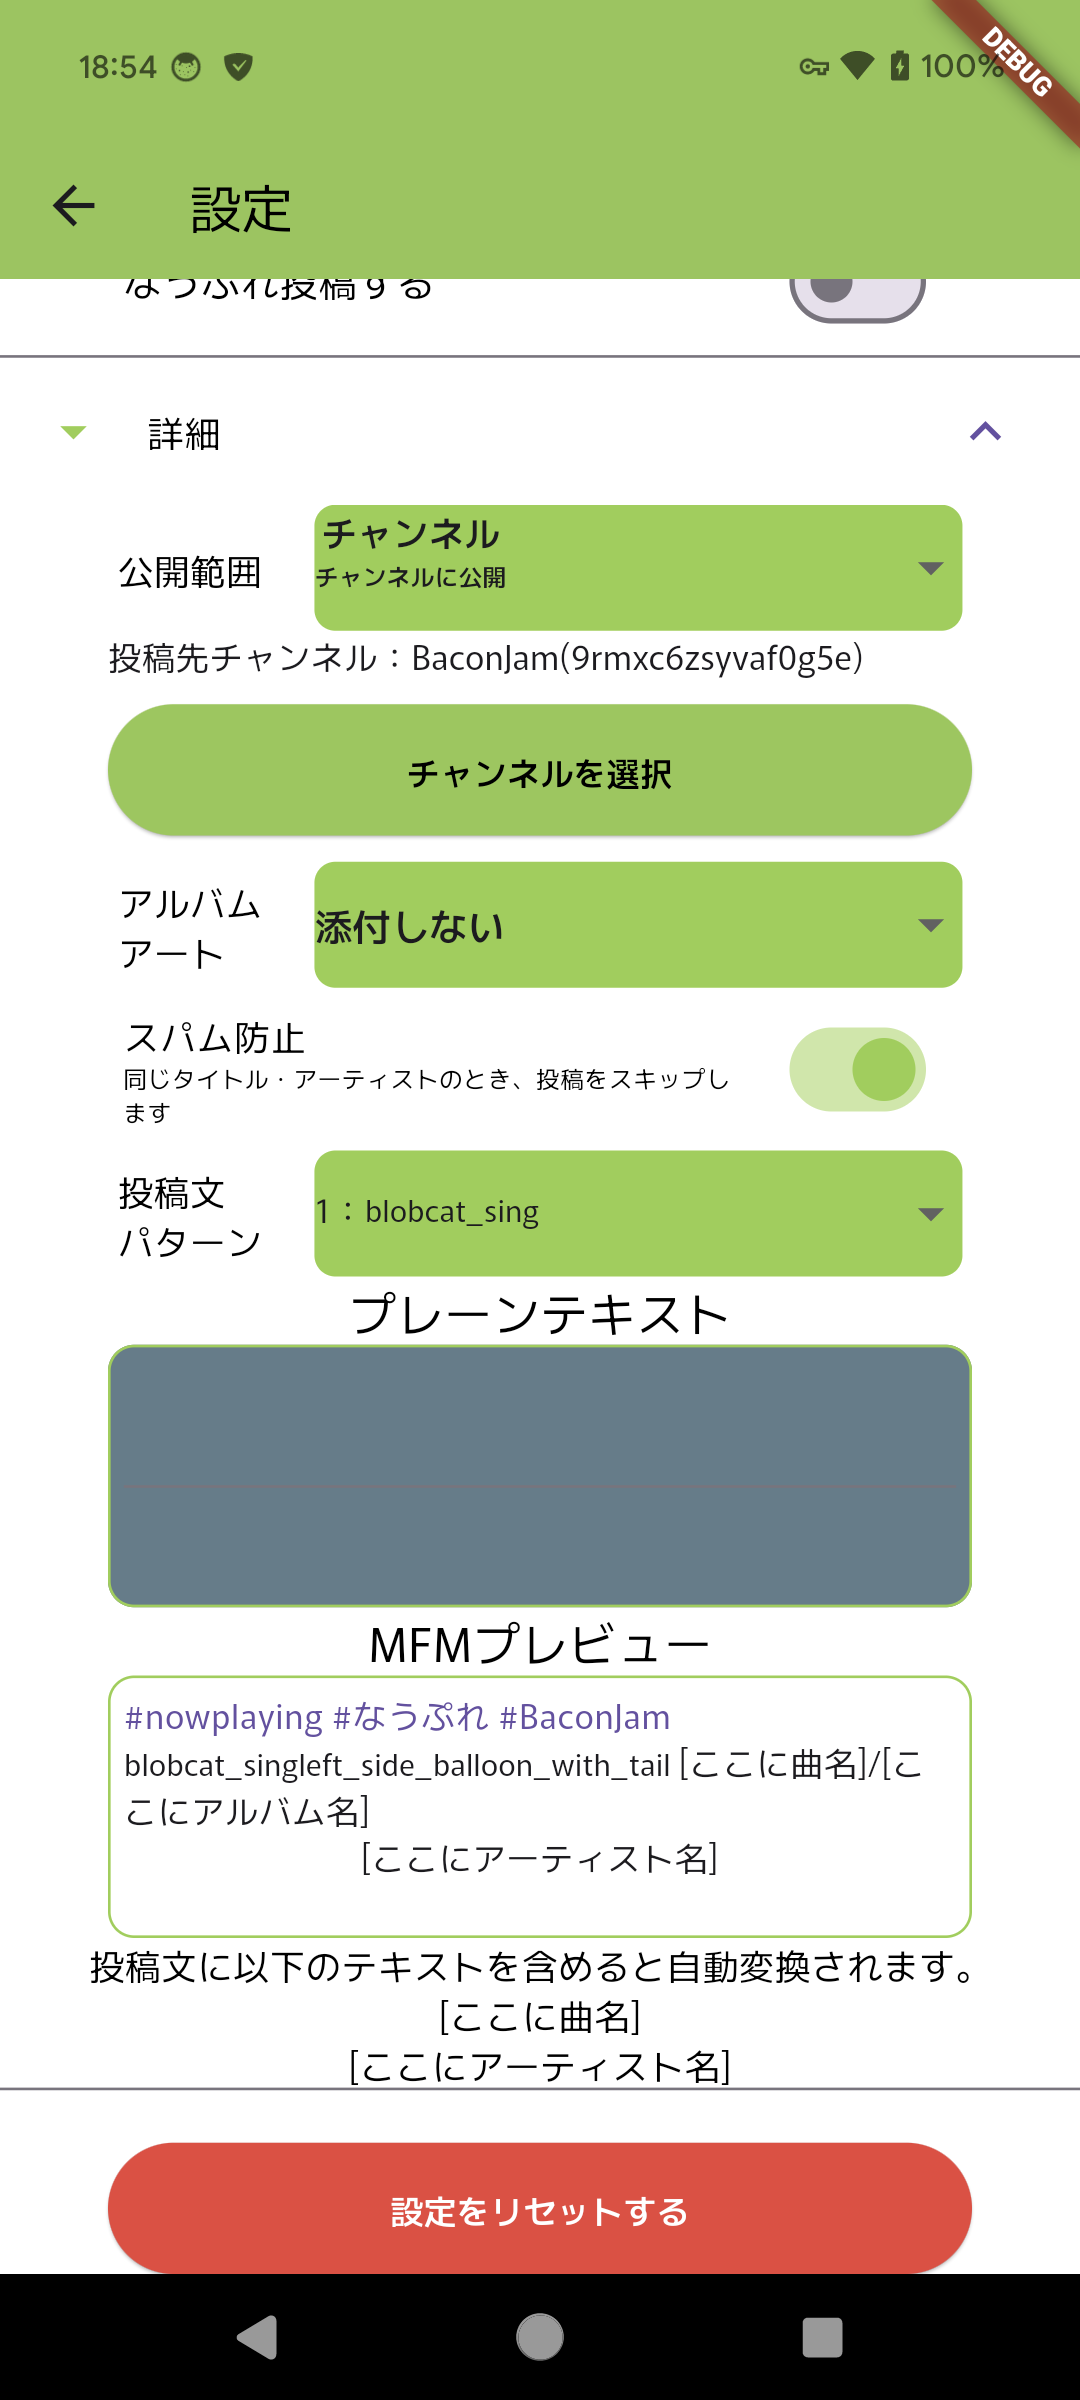
\includegraphics[width=5cm]{./pictures/guide6.png}
                }
                \caption{チャンネル指定後(\currentVersion)}
                \label{img:guide6}
            \end{figure}
    \end{enumerate}


\newpage
\section{バッテリー使用量の最適化}
\label{sec:battery1}
    \begin{enumerate}
        \item スマートフォンの\ttbox{設定}→\ttbox{アプリ}を押下してください。
            \begin{figure}[htbp]
                \centering
                \fbox{
                    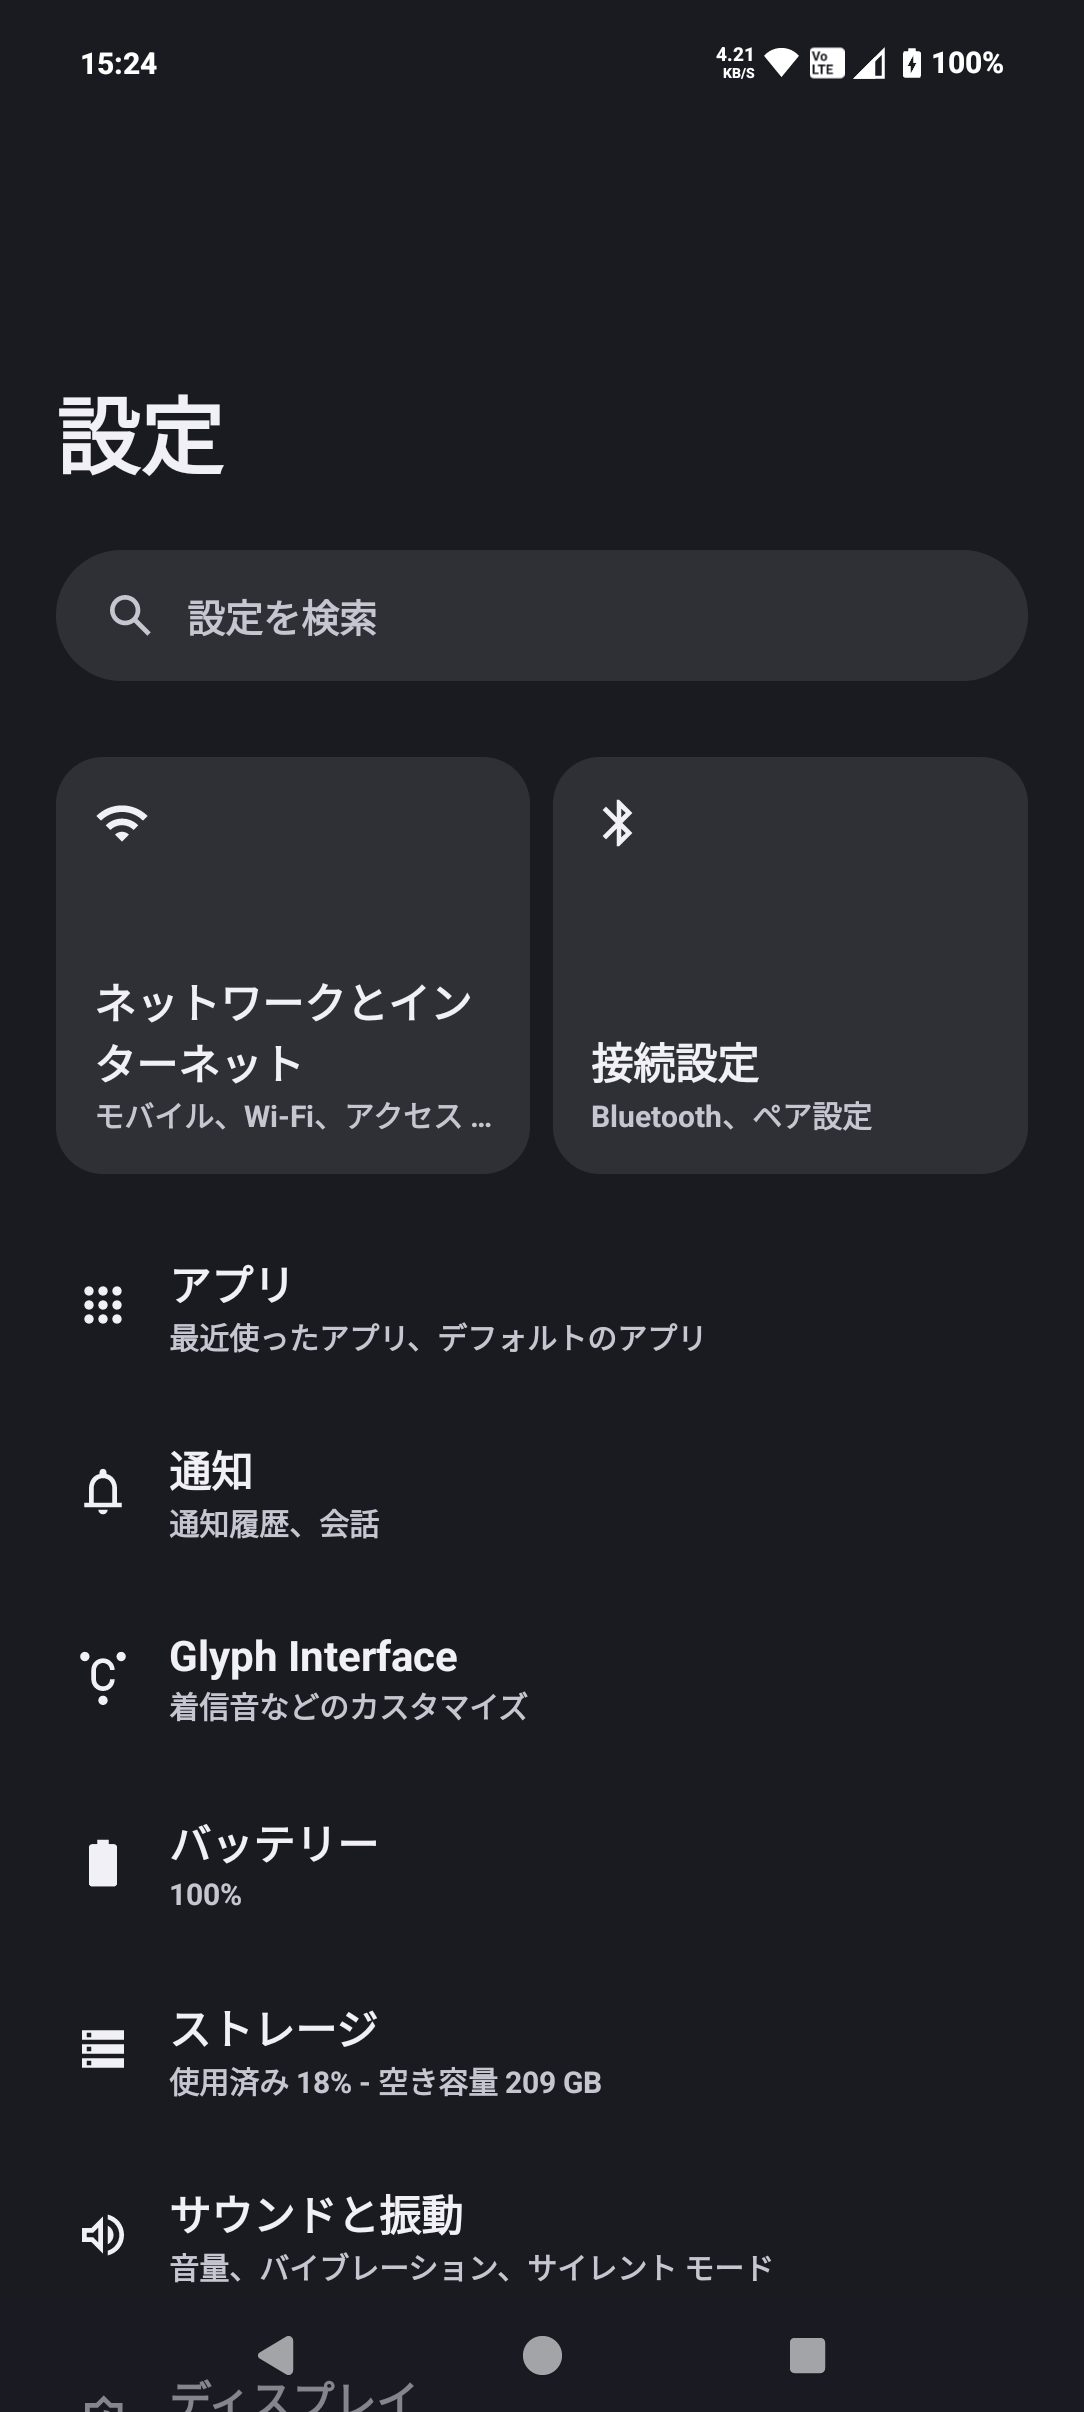
\includegraphics[width=5cm]{./pictures/battery1.png}
                }
                \caption{設定画面}
                \label{img:battery1}
            \end{figure}

        \newpage
        \item アプリ一覧の \bj を押下してください。
        \item \bj のアプリ情報画面の\ttbox{アプリのバッテリー使用量}を押下してください。
            \begin{figure}[htbp]
                \centering
                \fbox{
                    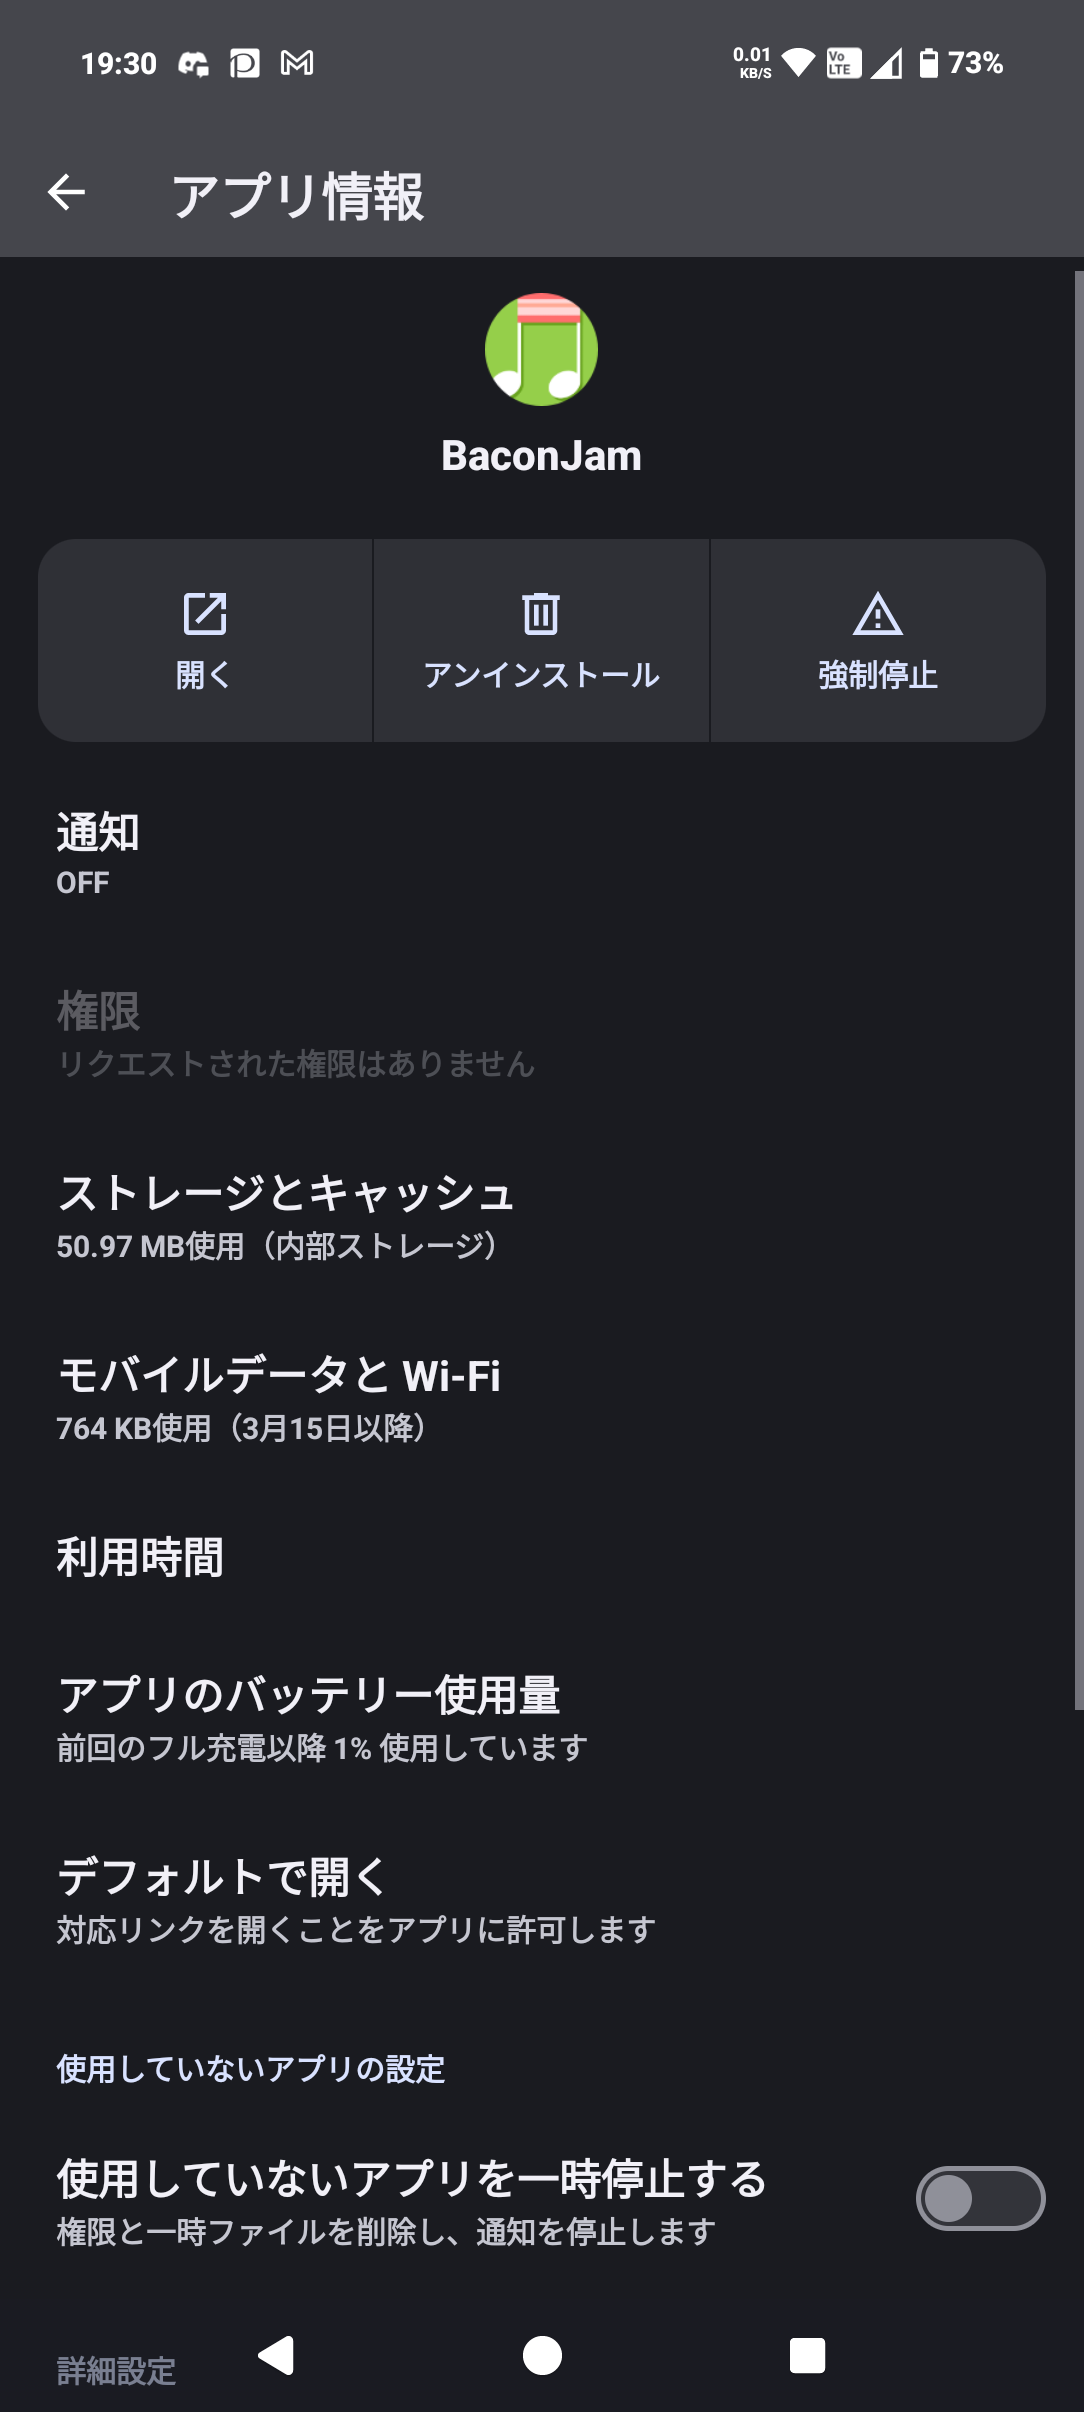
\includegraphics[width=5cm]{./pictures/battery2.png}
                }
                \caption{アプリの情報画面}
                \label{img:battery2}
            \end{figure}

        \newpage
        \item アプリのバッテリー使用量画面に表示されている
            \begin{itemize}
                \item 制限なし
                \item 最適化
                \item 制限
            \end{itemize}
            の中から、\ttbox{制限なし}を選択してください。
            \begin{figure}[htbp]
                \centering
                \fbox{
                    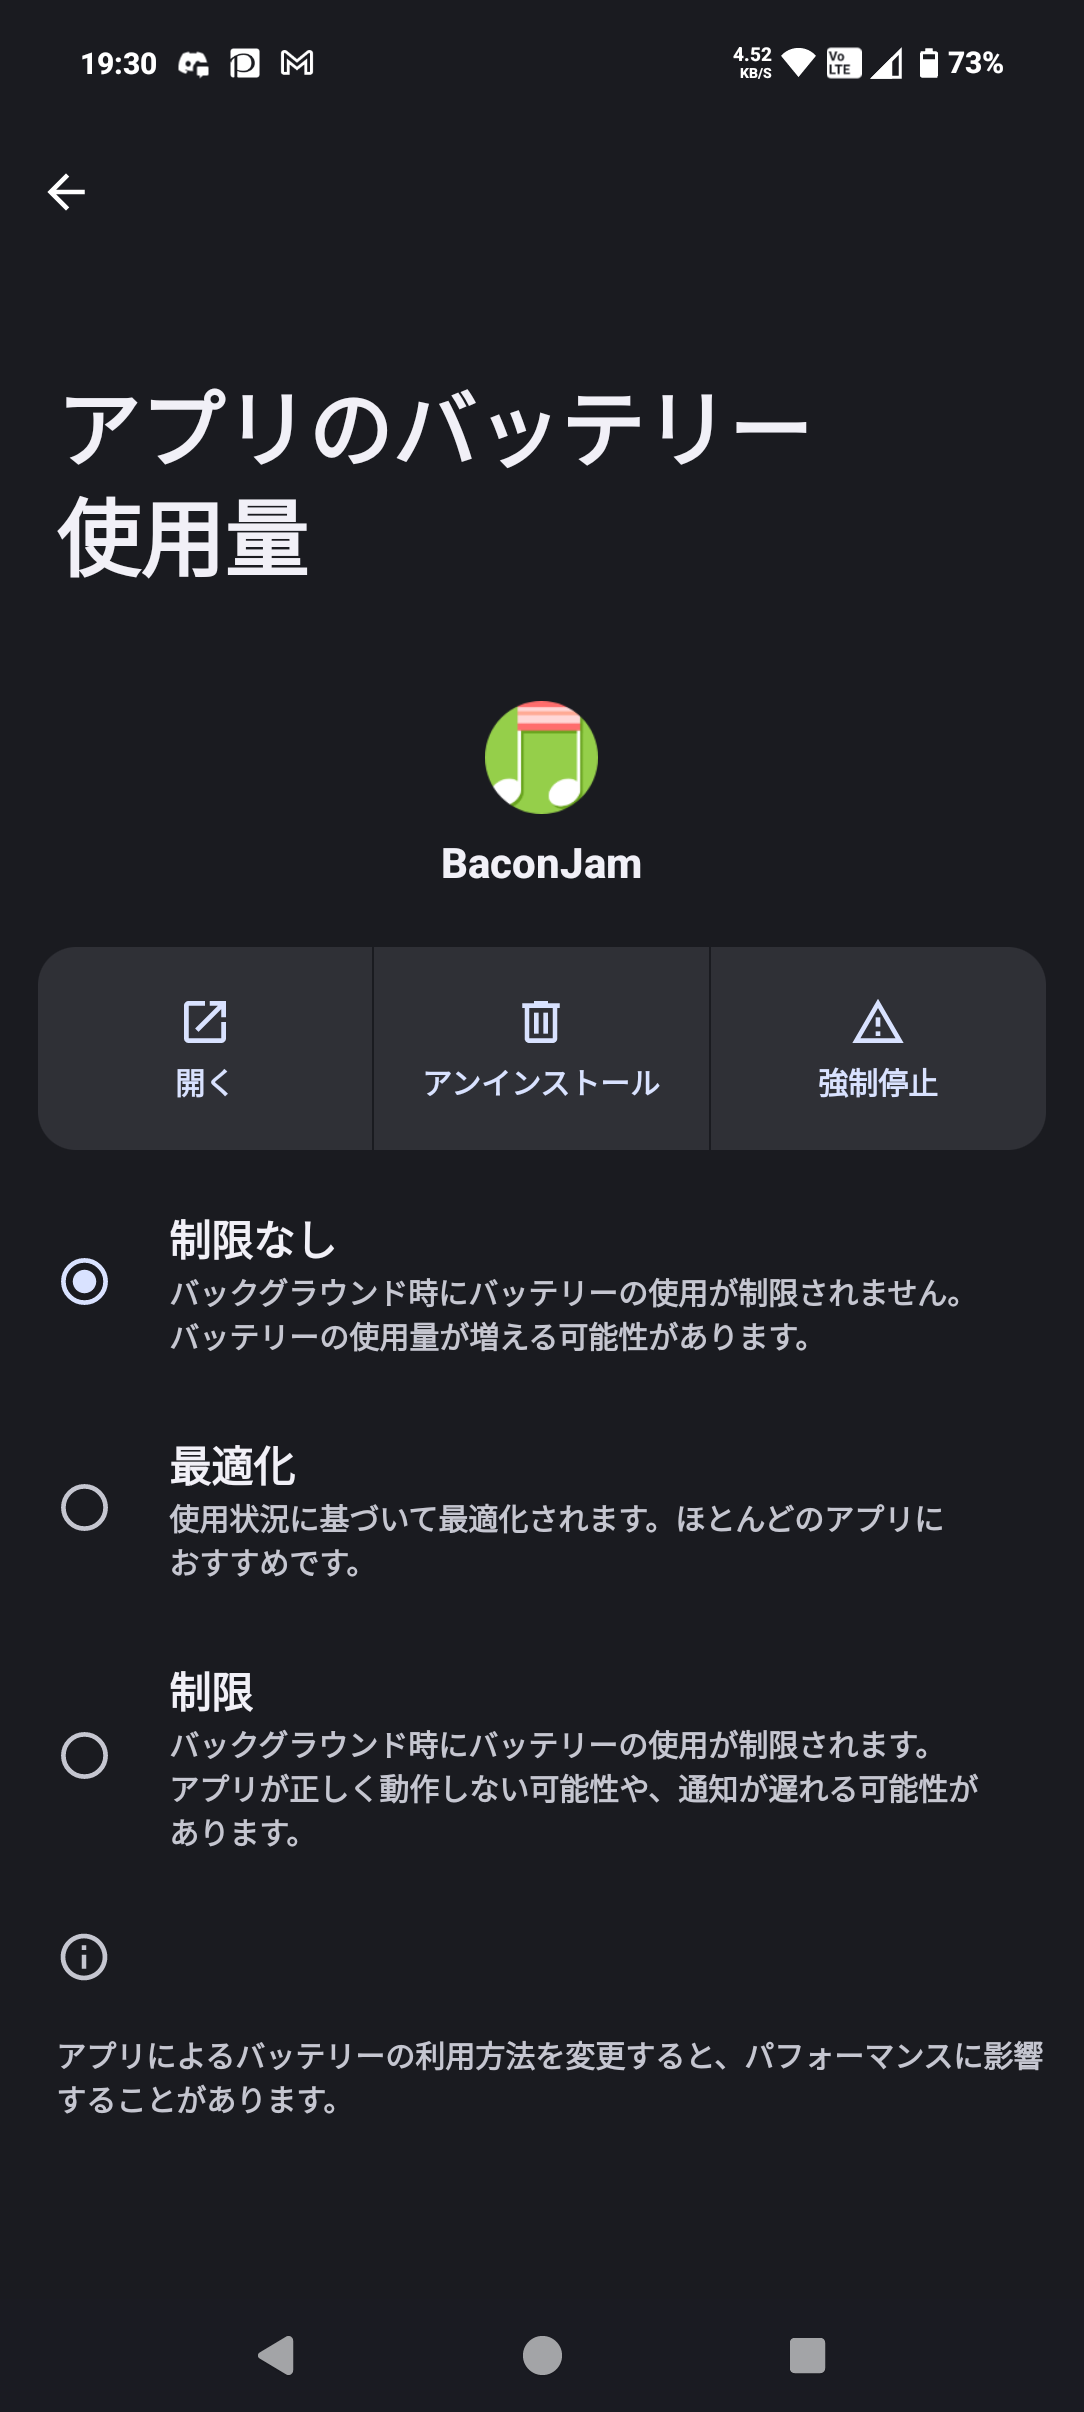
\includegraphics[width=5cm]{./pictures/battery3.png}
                }
                \caption{アプリのバッテリー使用量画面}
                \label{img:battery3}
            \end{figure}
    \end{enumerate}

\newpage
\section{リリースノート}
\subsection*{バージョンコード2(1.0.0)}
\begin{itemize}
    \item[リリース日] 2024年3月28日
\end{itemize}

\new
\begin{itemize}
    \item クローズドテストを開始しました。
\end{itemize}

\change \par
\fix

\newpage
\subsection*{バージョンコード3(1.1.0)}
\addcontentsline{toc}{subsection}{バージョンコード3(1.1.0)}
\begin{itemize}
    \item[リリース日] 2024年4月7日
\end{itemize}

\new
\begin{itemize}
    \item \nowplaying の公開範囲を以下から選択できる機能を追加しました。
        \begin{enumerate}
            \item パブリック(全てのユーザーに公開)
            \item ホーム(ホームタイムラインのみに公開)
            \item フォロワー(自分のフォロワーのみに公開)
            \item チャンネル\footnote{チャンネルIDの設定が必要です}
        \end{enumerate}
    \item Spotifyとの連携機能(プレビュー版)を追加しました。
    \item 設定画面に\ttbox{設定をリセットする}ボタンを追加しました。
\end{itemize}

\change
\begin{itemize}
    \item \nowplaying の際に以下の順にアーティスト名を取得し、最初に見つかったものを表示するように変更しました。
        \begin{enumerate}
            \item アルバムアーティスト名
            \item トラックアーティスト名
            \item 著者名
            \item 作者名
        \end{enumerate}
    \item \mi のアクセストークンが空欄の場合、\ttbox{テスト接続}ボタンを押下できないように変更しました。
    \item 設定画面の各種項目を折りたためるようにUIを変更しました。
\end{itemize}

\fix
\begin{itemize}
    \item ランキング画面の不要な\ttbox{TEST}ボタンを削除しました。
    \item 初回インストール時に投稿パターンの初期値が設定されておらず、\nowplaying できない不具合を修正しました。
\end{itemize}

\newpage
\subsection*{バージョンコード4(1.1.1)}
\addcontentsline{toc}{subsection}{バージョンコード4(1.1.1)}
\begin{itemize}
    \item[リリース日] 2024年4月8日
\end{itemize}

\new \par
\change
\begin{itemize}
    \item \mi との連携方法を変更しました。
\end{itemize}

\fix
\begin{itemize}
    \item 投稿パターン選択用ドロップダウンの挙動の不具合を修正しました。
\end{itemize}

\newpage
\subsection*{バージョンコード5(1.1.2)}
\begin{itemize}
    \item[リリース日] 2024年4月8日
\end{itemize}

\new \par
\change \par
\fix
\begin{itemize}
    \item \mi との連携操作の不具合を修正しました。
\end{itemize}

\newpage
\subsection*{バージョンコード6(1.1.3)}
\begin{itemize}
    \item[リリース日] 2024年4月8日
\end{itemize}

\new \par
\change \par
\fix
\begin{itemize}
    \item \nowplaying 時の挙動不具合を修正しました。
\end{itemize}

\newpage
\subsection*{バージョンコード7(1.2.0)}
\begin{itemize}
    \item[リリース日] 2024年4月8日
\end{itemize}

\new \par
\change
\begin{itemize}
    \item \nowplaying の投稿先チャンネルを名称またはIDで検索して指定できるように変更しました。
    \item \bj 全体のフォントを\href{https://fonts.google.com/specimen/Murecho?subset=japanese}{Murecho}に変更しました。
\end{itemize}

\fix

\newpage
\subsection*{バージョンコード8(1.2.1)}
\addcontentsline{toc}{subsection}{バージョンコード8(1.2.1)}
\begin{itemize}
    \item[リリース日] 2024年4月11日
\end{itemize}

\new \par
\change \par
\fix
\begin{itemize}
    \item \clientId ,\clientSecret を入力した際の\ttbox{接続テスト}ボタンの挙動の不具合を修正しました。
\end{itemize}


\newpage
\subsection*{バージョンコード9(1.2.2)}
\addcontentsline{toc}{subsection}{バージョンコード9(1.2.2)}
\begin{itemize}
    \item[リリース日] 2024年4月12日
\end{itemize}

\new
\begin{itemize}
    \item Spotifyの曲を投稿する際、曲のURLを添付する機能を追加しました。
\end{itemize}

\change
\begin{itemize}
    \item \nowplaying のオンオフを変更した際、トーストメッセージを表示するように変更しました。
\end{itemize}

\fix
\begin{itemize}
    \item \nowplaying のオンオフがSpotifyの投稿機能と連動しない不具合を修正しました。
\end{itemize}


\newpage
\subsection*{バージョンコード10(1.2.3)}
\addcontentsline{toc}{subsection}{バージョンコード10(1.2.3)}
\begin{itemize}
    \item[リリース日] 2024年4月13日
\end{itemize}

\new \par
\change
\begin{itemize}
    \item ハンバーガーメニュー内の広告をテスト用から実際の広告に変更しました。
\end{itemize}

\fix


\newpage
\subsection*{バージョンコード11(1.2.4)}
\addcontentsline{toc}{subsection}{バージョンコード11(1.2.4)}
\begin{itemize}
    \item[リリース日] 2024年4月14日
\end{itemize}

\new \par
\change
\begin{itemize}
    \item ハンバーガーメニュー内のUIを変更しました。
\end{itemize}

\fix


\newpage
\subsection*{バージョンコード12(1.2.5)}
\addcontentsline{toc}{subsection}{バージョンコード12(1.2.5)}
\begin{itemize}
    \item[リリース日] 2024年4月15日
\end{itemize}

\new \par
\change \par
\fix
\begin{itemize}
    \item 起動できなくなる不具合を修正しました。
\end{itemize}



\newpage
\subsection*{バージョンコード13(1.2.6)}
\addcontentsline{toc}{subsection}{バージョンコード13(1.2.6)}
\begin{itemize}
    \item[リリース日] 2024年4月15日
\end{itemize}

\new \par
\change \par
\fix
\begin{itemize}
    \item 軽微な修正を行いました。
\end{itemize}



\newpage
\subsection*{バージョンコード16(1.2.9)}
\addcontentsline{toc}{subsection}{バージョンコード16(1.2.9)}
\begin{itemize}
    \item[リリース日] 2024年4月16日
\end{itemize}

\new
\begin{itemize}
    \item ハンバーガーメニューに連携している\mi のプロフィールを表示する機能を追加しました。
    \item ハンバーガーメニューに感想用Googleフォームへのリンクを追加しました。
\end{itemize}

\change \par
\fix
\begin{itemize}
    \item 軽微なUIの修正を行いました。
\end{itemize}



\newpage
\subsection*{バージョンコード21(1.3.4)}
\addcontentsline{toc}{subsection}{バージョンコード21(1.3.4)}
\begin{itemize}
    \item[リリース日] 2024年4月23日
\end{itemize}

\new
\begin{itemize}
    \item プレイリスト作成・再生機能を追加しました。
\end{itemize}

\change
\begin{itemize}
    \item クローズドテストから製品版(一般公開)にリリース先を変更しました。
\end{itemize}

\fix
\begin{itemize}
    \item 軽微なUIの修正を行いました。
\end{itemize}



\newpage
\subsection*{バージョンコード23(1.3.6)}
\addcontentsline{toc}{subsection}{バージョンコード23(1.3.6)}
\begin{itemize}
    \item[リリース日] 2024年4月24日
\end{itemize}

\new
\begin{itemize}
    \item 前の曲へボタン、次の曲へボタンを追加しました。
\end{itemize}

\change
\begin{itemize}
    \item プレイリストを再生ボタン、音楽ファイルを再生ボタンの配置を変更しました。
    \item プレイリスト未作成の場合の画面デザインを変更しました。
    \item ランキングデータなしの場合の画面デザインを変更しました。
\end{itemize}

\fix


\newpage
\subsection*{バージョンコード24(1.3.7)}
\addcontentsline{toc}{subsection}{バージョンコード24(1.3.7)}
\begin{itemize}
    \item[リリース日] 2024年4月27日
\end{itemize}

\new
\begin{itemize}
    \item 曲名、アーティスト名、アルバム名の\verb|#|を\verb|#|に置換しハッシュタグ化を防ぐ処理を追加しました。
\end{itemize}

\change
\begin{itemize}
    \item \mi 連携、Spotify連携の画面をアプリ内ブラウザ表示から外部ブラウザ表示に変更しました。
\end{itemize}

\fix



\newpage
\subsection*{バージョンコード25(1.3.8)}
\addcontentsline{toc}{subsection}{バージョンコード25(1.3.8)}
\begin{itemize}
    \item[リリース日] 2024年4月28日
\end{itemize}

\new
\begin{itemize}
    \item \href{https://misskey-hub.net/ja/servers/}{Misskey Hubのサーバー一覧}に掲載されていないサーバーでも接続先として指定できる機能を追加しました。
    \item ライトテーマ・ダークテーマ変更時にポップアップ通知を表示する機能を追加しました。
\end{itemize}

\change
\begin{itemize}
    \item 接続先サーバー変更時に、カスタム絵文字を自動的に取得するように変更しました。
\end{itemize}

\fix



\newpage
\subsection*{バージョンコード26(1.3.9)}
\addcontentsline{toc}{subsection}{バージョンコード26(1.3.9)}
\begin{itemize}
    \item[リリース日] 2024年4月30日
\end{itemize}

\new
\begin{itemize}
    \item ハンバーガーメニューのアイコンを押下すると\mi のプロフィールにジャンプする機能を追加しました。
    \item \nowplaying の際に以下に含まれる\verb|:|を\verb|:|に置換し、カスタム絵文字の表示が崩れないようにする機能を追加しました。
        \begin{itemize}
            \item 曲名
            \item アーティスト名
            \item アルバム名
        \end{itemize}
\end{itemize}

\change

\fix



\newpage
\subsection*{バージョンコード27(1.4.0)}
\addcontentsline{toc}{subsection}{バージョンコード27(1.4.0)}
\begin{itemize}
    \item[リリース日] 2024年5月1日
\end{itemize}

\new

\change
\begin{itemize}
    \item サポート対象のandroid OSを13以上から5以上に拡張しました。
\end{itemize}

\fix



\newpage
\subsection*{バージョンコード28(1.4.1)}
\addcontentsline{toc}{subsection}{バージョンコード28(1.4.1)}
\begin{itemize}
    \item[リリース日] 2024年5月3日
\end{itemize}

\new
\begin{itemize}
    \item 外部ストレージの音楽ファイル読み込み機能を追加しました。
\end{itemize}

\change

\fix



\newpage
\section{各種連絡先}
\label{contact}
    \begin{itemize}
        \item[Misskey.io] \href{https://misskey.io/@96ENU}{\texttt{@96ENU}}
        \item[Twitter] \href{https://twitter.com/96ENU}{\texttt{@96ENU}}
        \item[Mail] \verb|96enu.illustration@gmail.com|
        \item[Discord]
            \begin{itemize}
                \item 個人:\verb|96ENU|
                \item \bj 用サーバ:\href{https://discord.gg/C3veaKqp}{Join to Server}
            \end{itemize}
    \end{itemize}

\newpage
\appendix
\section{\currentVersion がサポートしているデバイス一覧}
\label{sec:supporteddevices}
\setlongtables
\begin{tabularx}{\linewidth}{|l|X|X|}
    \hline
        \cellcolor{gray}メーカー & \cellcolor{gray}デバイス名 & \cellcolor{gray}モデル名 \\ \hline
        \endhead

        8849 & TANK2 & TANK2 \\ \hline
        AAUW & T60Pro 2023 & T60Pro 2023 \\ \hline
        AAUW & T50 2023 & T50 2023 \\ \hline
        AAUW & T90 & T90 \\ \hline
        ACE & BUZZ 4Pro & BUZZ 4Pro \\ \hline
        ACE & BUZZ 4 Prime & BUZZ 4 Prime \\ \hline
        ACE & BUZZ 4Lite & BUZZ 4Lite \\ \hline
        ACE & BUZZ 4 Ultra & BUZZ 4 Ultra \\ \hline
        ACE & BUZZ 4 Note & AS0623 \\ \hline
        ACER & Acer A60L & Acer A60L \\ \hline
        ADVAN & ADVAN TAB VX LITE & VX LITE \\ \hline
        ADVAN & ADVAN SKETSA3 & Sketsa3 \\ \hline
        ADVAN & ADVAN XTAB & XTAB \\ \hline
        ADVANCE & SP7348 & SP7348 \\ \hline
        AGM & AGM PAD P1 & AGM PAD P1 \\ \hline
        AGM & AGM Note N1 & AGM Note N1 \\ \hline
        AGM & AGM H6 & AGM H6 \\ \hline
        AHA & AHA ULTRA RK3588 & IFPD \\ \hline
        ALIGATOR & RX850 & RX850 \\ \hline
        ALLVIEW & V10 Viper & V10 Viper \\ \hline
        ALT & odin & ODIN Kids Phone \\ \hline
        ALTICE & S35 & ALTICE S35 \\ \hline
        ALTICE & E55 & Altice E55 \\ \hline
        ASPERA & ASPERA R10 & ASPERA R10 \\ \hline
        ATMPC & IT-1001A & IT-1001A \\ \hline
        ATOZEE & CP20 PRO & CP20 PRO \\ \hline
        ATOZEE & CP20 MAX & CP20 MAX \\ \hline
        ATOZEE & YQ10S Gold & YQ10S Gold \\ \hline
        ATOZEE & YQ10S MAX & YQ10S MAX \\ \hline
        ATOZEE & CP30 & CP30 \\ \hline
        ATT & U380AA & AT\&T Calypso® 4 \\ \hline
        ATT & U6080AA & AT\&T Propel™ 5G \\ \hline
        ATT & WTATTRW2 & WTATTRW2 \\ \hline
        AURZEN & TB-AS100A & TB-AS100A \\ \hline
        AVA & AVA-RM-RX2-US & AVA-RM-RX2-US \\ \hline
        AXEL & AX PRO & AX PRO \\ \hline
        Acer & AcerOne8T9-422L & Acer One 8 T9-422L \\ \hline
        Achate & KidsTab3 EEA & KidsTab3 EEA \\ \hline
        Adreamer & LeoPad 10X & LeoPad 10X \\ \hline
        Alldocube & U1030 & iPlay50 Lite \\ \hline
        Alldocube & T1029TA & iPlay50S \\ \hline
        Alldocube & T1030X & iPlay50 \\ \hline
        Alldocube & U807 & iPlay50 Mini Lite \\ \hline
        Alldocube & T1030MAN & iPlay 50 Pro \\ \hline
        Alldocube & T1102T & iPlay 60 \\ \hline
        Alldocube & KidzPad Pro & KidzPad Pro \\ \hline
        Allnet & PrimeOne & PrimeOne \\ \hline
        Amobile & PD602 & PD602 \\ \hline
        AngelTech & P80 & P80 \\ \hline
        Aocwei & X700 EEA & X700 EEA \\ \hline
        Aocwei & X500 T EEA & X500 T EEA \\ \hline
        Apolosign & K709A & K709A \\ \hline
        Apolosign & EM101A & EM101A \\ \hline
        Apolosign & K109A & K109A \\ \hline
        Apolosign & EM103A & EM103A \\ \hline
        Aspera & AS5 & AS5 \\ \hline
        Aspera & AS57 & AS57 \\ \hline
        Aspera & AS8 & AS8 \\ \hline
        Aspera & Nitro2 & Nitro2 \\ \hline
        Athesi & AP5501 & AP5501 \\ \hline
        Ayat & Ayat101 & Ayat101 \\ \hline
        BENEVE & M55 & M55 \\ \hline
        BENEVE & M55 EEA & M55 EEA \\ \hline
        BENEVE & M51S & M51S \\ \hline
        BENEVE & M51S EEA & M51S EEA \\ \hline
        BLOW & PlatinumTAB11 4G & PlatinumTAB11 4G \\ \hline
        BLU & G0771 & G73 \\ \hline
        BLU & G0892 & G33 \\ \hline
        BLU & M0215 ND & M10L Pro \\ \hline
        BLU & J0140 & J10L \\ \hline
        BLU & G0860 & G63 \\ \hline
        BLU & N0070 & BOLD N3 \\ \hline
        BLU & G0870 & G63 \\ \hline
        BLU & G0850 & G53 \\ \hline
        BLU & B160V & B160V \\ \hline
        BLU & J0150 & J10L \\ \hline
        BLU & G0930 & G73L \\ \hline
        BLU & C0200 & C6L MAX \\ \hline
        BLU & C0175 & C5L Max \\ \hline
        BLU & G0910 & G93 \\ \hline
        BLU & G0950 & G43 \\ \hline
        BLU & G0850 IW & G53 \\ \hline
        BLU & M0178 ND & M10L \\ \hline
        BLU & G0851 & G53 \\ \hline
        BLU & G0890 & G33 \\ \hline
        BLU & B170D & View 5 Pro \\ \hline
        BMAX & I9 Plus WLAN EEA & I9 Plus WLAN EEA \\ \hline
        BMAX & I11 Power & I11 Power \\ \hline
        BMAX & I9 Plus WLAN & I9 Plus WLAN \\ \hline
        BenQ & RP7504 & RP7504 \\ \hline
        BenQ & RM6504 & RM6504 \\ \hline
        BenQ & RM8604 & RM8604 \\ \hline
        BenQ & RP8604 & RP8604 \\ \hline
        BenQ & RP6504 & RP6504 \\ \hline
        BenQ & RM7504 & RM7504 \\ \hline
        Benten & Benten T30 & Benten T30 \\ \hline
        Blackview & BV6200 & BV6200 \\ \hline
        Blackview & Tab10WiFi & Tab 10 WiFi \\ \hline
        Blackview & N6000 & N6000 \\ \hline
        Blackview & Active8Pro & Active 8 Pro \\ \hline
        Blackview & BV9300 Pro & BV9300 Pro \\ \hline
        Blackview & BV8900 & BV8900 \\ \hline
        Blackview & Active6 EEA & Active 6 \\ \hline
        Blackview & Tab70WiFi & Tab 70 WiFi \\ \hline
        Blackview & Tab60 & Tab 60 \\ \hline
        Blackview & Tab80 EEA & Tab 80 \\ \hline
        Blackview & BV5300 Plus & BV5300 Plus \\ \hline
        Blackview & Tab50WiFi & Tab50WiFi EEA \\ \hline
        Blackview & A96 & A96 \\ \hline
        Blackview & Tab13 Pro & Tab 13 Pro \\ \hline
        Blackview & Tab80 RU & Tab 80 \\ \hline
        Blackview & BV6200Pro & BV6200 Pro \\ \hline
        Blackview & Active6 & Active 6 \\ \hline
        Blackview & Tab3Kids & Tab 3 Kids \\ \hline
        Blackview & A200Pro & A200 Pro \\ \hline
        Blackview & Tab80 & Tab 80 \\ \hline
        Blackview & Tab60Kids EEA & Tab 60 Kids \\ \hline
        Blaupunkt & BP T6110X & BP T6110X \\ \hline
        Blaupunkt & BP T6108X & BP T6108X \\ \hline
        Bmobile & Bmobile BL55 & BL55 \\ \hline
        Bmobile & Bmobile BL53 TG05 & BL53 \\ \hline
        Bmobile & Bmobile BL53 TG06 & BL53 \\ \hline
        Bmobile & Bmobile BL63Pro & BL63Pro \\ \hline
        Bmobile & Bmobile BL65Plus TG07 & BL65Plus TG07 \\ \hline
        Bmobile & Bmobile BL53 TG07 & BL53 \\ \hline
        Byybuo & SmartPad A70W & SmartPad A70W \\ \hline
        Byybuo & SmartPad A10 EU & SmartPad A10 EU \\ \hline
        Byybuo & SmartPad A10 L & SmartPad A10 L \\ \hline
        CHUWI & Hi10 XPro & Hi10 XPro \\ \hline
        COIN & 1200AS plus & 1200AS plus \\ \hline
        COLORROOM & K12 & K12 \\ \hline
        COOLFAN & OC106 & OC106 \\ \hline
        CUBOT & KINGKONG 8 & KINGKONG 8 \\ \hline
        CUBOT & NOTE 40 & NOTE 40 \\ \hline
        CUBOT & TAB 20 & TAB 20 \\ \hline
        CUBOT & TAB 40 & TAB 40 \\ \hline
        CUBOT & TAB 50 & TAB 50 \\ \hline
        CUBOT & KINGKONG STAR & KINGKONG STAR \\ \hline
        CUBOT & NOTE 50 & NOTE 50 \\ \hline
        CUBOT & KINGKONG 9 & KINGKONG 9 \\ \hline
        CUBOT & X30P & X30P \\ \hline
        CUBOT & TAB KINGKONG & TAB KINGKONG \\ \hline
        CUBOT & P80 & P80 \\ \hline
        CUBOT & X70 & X70 \\ \hline
        CWOWDEFU & P15W EEA & P15W EEA \\ \hline
        CWOWDEFU & P15W & P15W \\ \hline
        Casper & VIA A40 & VIA A40 \\ \hline
        Casper & VIA X40 & VIA X40 \\ \hline
        Casper & VIA M35 & VIA M35 \\ \hline
        Casper & VIA X30 Plus & VIA X30 Plus \\ \hline
        Casper & VIA X30 & VIA X30 \\ \hline
        Casper & VIA L40 & VIA L40 \\ \hline
        Cidea & CM826 & CM826 \\ \hline
        Cidea & CM90 & CM90 \\ \hline
        Cidea & CM91 EEA & CM91 EEA \\ \hline
        Cidea & P1100 & P1100 \\ \hline
        ClearTouch & rk3588 t & six zero XXAplus \\ \hline
        Clevertouch & rk3588 t & IMPACT Lux \\ \hline
        Compaq & Qtab10Plus & Qtab10Plus \\ \hline
        Compaq & Qtab10 & Qtab 10.1 with keyboard \\ \hline
        Compaq & Qtab & QTabPro \\ \hline
        Coolpad & CP12t & 3631 \\ \hline
        Cricket & U6080AC & Cricket® Magic 5G \\ \hline
        Cricket & U380AC & Cricket Debut S2™ \\ \hline
        Crosscall & L780 & Stellar-X5 \\ \hline
        Crosscall & L790 & Core-Z5 \\ \hline
        D-TECH & DT10-TAB4G-T101 & DT10-TAB4G-T101 \\ \hline
        DABLIU & E13R B75G & E13R \\ \hline
        DABLIU & rk3588 E13R & E13R B65G \\ \hline
        DEPLAY & BS801 EEA & BS801 \\ \hline
        DEWSOD & C9 & C9 \\ \hline
        DIALN & X10ULTRA & X10ULTRA \\ \hline
        DIALN & S8 & S8 \\ \hline
        DIALN & G65 & G65 \\ \hline
        DIALN & S10 & S10 \\ \hline
        DIALN & X10G & X10G \\ \hline
        DIALN & X8G & X8G \\ \hline
        DIALN & G10 & G10 \\ \hline
        DOCOMO & SH-52D & AQUOS R8 \\ \hline
        DOCOMO & SH-54B & AQUOS sense6 \\ \hline
        DOCOMO & SH-54D & AQUOS sense8 \\ \hline
        DOCOMO & SH-53D & AQUOS wish3 \\ \hline
        DOCOMO & SH-51C & AQUOS wish2 \\ \hline
        DOCOMO & SH-51D & AQUOS R8 pro \\ \hline
        DOCOMO & SH-53C & AQUOS sense7 \\ \hline
        DOCOMO & SH-51B & AQUOS R6 \\ \hline
        DOCOMO & SH-52C & AQUOS R7 \\ \hline
        DOCOMO & SH-53A & AQUOS sense5G \\ \hline
        DOMATON & D718 & D718 \\ \hline
        DOOGEE & M21TE & S41 \\ \hline
        DOOGEE & P3Mini & T20Mini \\ \hline
        DOOGEE & M23S & V31GT \\ \hline
        DOOGEE & PT1 & R10 \\ \hline
        DOOGEE & P3Mini Kid & P3Mini Kid \\ \hline
        DOOGEE & M22P & S110 \\ \hline
        DOOGEE & P1D & T10S \\ \hline
        DOOGEE & P4 & T10SE \\ \hline
        DOOGEE & ZN137 & Smini \\ \hline
        DOOGEE & 1918Y & N50 \\ \hline
        DOOGEE & P3Pro & T30Pro \\ \hline
        DOOGEE & RK1KID & U10KID \\ \hline
        DOOGEE & 1918D & N50S \\ \hline
        DOOGEE & P2D & T20S \\ \hline
        DOOGEE & RK1 & U10 \\ \hline
        DREAMTECH & STARPAD & STARPAD \\ \hline
        DUODUOGO & S8 & S8 \\ \hline
        Danew & Dslide 809Pro & Dslide 809Pro EEA \\ \hline
        Datamini & T104G & T104G T618 \\ \hline
        DeutscheTelekom & Tiger & T Phone Pro (2023) \\ \hline
        DeutscheTelekom & Leopard & T Phone (2023) \\ \hline
        DeutscheTelekom & Lion & T Phone Pro \\ \hline
        DeutscheTelekom & Hubbs & T Tablet \\ \hline
        DeutscheTelekom & Jaguar & T Phone \\ \hline
        Dialn & Neo & Neo \\ \hline
        Dialn & X62 & X62 \\ \hline
        Dialn & X62B & X62 \\ \hline
        Dialn & X65B & X65 \\ \hline
        Dialn & X65C & X65 \\ \hline
        Dialn & X62A & X62 \\ \hline
        Dialn & NeoA & Neo \\ \hline
        Dialn & X62C & X62 \\ \hline
        Dialn & Nova & Nova \\ \hline
        Dialn & NovaA & Nova \\ \hline
        Dialn & X65A & X65 \\ \hline
        Dijitsu & DCT 90 & DCT 90 \\ \hline
        Dish & U653DS & Celero3 5G \\ \hline
        Dish & U695DS & Celero3 5G+ \\ \hline
        EagleSoar & EE10A & EE10A \\ \hline
        Ehlel & Ehlel Defender D23 & Defender \\ \hline
        Energizer & U506S & U506S \\ \hline
        Entity & ENTG1011 & ENTG1011 \\ \hline
        FACETEL & Q10-EEA & Q10-EEA \\ \hline
        FACETEL & W3 T US & W3 T US \\ \hline
        FACETEL & Q3 EEA & Q3 EEA \\ \hline
        FACETEL & Q10-US & Q10-US \\ \hline
        FACETEL & Q6 US & Q6 US \\ \hline
        FACETEL & W3 T EEA & W3 T EEA \\ \hline
        FCNT & F41B & arrows Be4 Plus F-41B \\ \hline
        FCNT & F51B & arrows We F-51B \\ \hline
        FCNT & A101FC & arrows We A101FC \\ \hline
        FCNT & FCG01 & arrows We FCG01 \\ \hline
        FCNT & F51C & arrows N F-51C \\ \hline
        FEONAL & D118 EEA & D118 EEA \\ \hline
        FOLG & KS20 & KS20 \\ \hline
        FOSSiBOT & F106 Pro & F106 Pro ROW \\ \hline
        FOSSiBOT & F101 Pro & F101 Pro \\ \hline
        FOSSiBOT & F101 P & F101 P \\ \hline
        FOSSiBOT & F102 & F102 \\ \hline
        FOXXD & C10 & C10 \\ \hline
        FOXXD & A56 & A56 \\ \hline
        FOXXD & FOXXD C65 & FOXXD C65 \\ \hline
        Fairphone & FP3 & Fairphone3 \\ \hline
        Fairphone & FP5 & Fairphone 5 5G \\ \hline
        Fairphone & FP4 & Fairphone4 \\ \hline
        Fivahiva & FF10A & FF10A \\ \hline
        FreeYond & F9S & F9S \\ \hline
        FreeYond & M6 & M6 \\ \hline
        FreeYond & M5A & M5A \\ \hline
        G-Tab & C10-pro & C10 \\ \hline
        G-Tab & C30 & C30 \\ \hline
        G-Tab & S50 & S50 \\ \hline
        G-mee & ConnectPro & ConnectPro \\ \hline
        GHIA & GVPNT & GVPNT \\ \hline
        GHIA & GK133 & GK133 \\ \hline
        GHIA & GA8N & GA8N \\ \hline
        GM & G316 & GM 23 Dual \\ \hline
        GM & G901 & GM Phoenix 5G d \\ \hline
        GM & G514 & GM 24 Pro \\ \hline
        GM & G314 & GM 23 SE Dual \\ \hline
        GREATASIA & E700 Kids EEA & E700 Kids EEA \\ \hline
        GREATASIA & E10 A133 EEA & E10 A133 EEA \\ \hline
        GTEL & Infinity 13 & Infinity 13 \\ \hline
        GTEL & Delta 14 & Delta 14 \\ \hline
        G Anica & HL 1088 A133P & HL 1088 A133P \\ \hline
        Gfast & MD 97 S464A & MD 97 S464A \\ \hline
        Gigaset & GX6 PRO & Gigaset GX6 PRO \\ \hline
        Gigaset & GS5 & GS5 \\ \hline
        Gigaset & GS5 LITE & GS5 LITE \\ \hline
        Gigaset & GX6 & Gigaset GX6 \\ \hline
        GlobalSec & BW819E CR EEA & BW819E CR \\ \hline
        GlobalSec & BW819E SK EEA & BW819E SK \\ \hline
        GreenLion & G-10 ULTRA & G-10 ULTRA \\ \hline
        GreenLion & G-10 PRO & G-10 PRO \\ \hline
        GreenLion & G-8 PRO & G-8 PRO \\ \hline
        H819E & MINTAKA & MINTAKA \\ \hline
        HAFURY & V1 & V1 \\ \hline
        HANNspree & Reader & HSD0001 \\ \hline
        HDC & T7I 232 & T7I 232 \\ \hline
        HEADWOLF & F2A & F2A \\ \hline
        HEADWOLF & Hpad5 & Hpad5 \\ \hline
        HEADWOLF & Fpad3 & Fpad3 \\ \hline
        HIGRACE & OC101 & OC101 \\ \hline
        HIGRACE & OC101 EEA & OC101 \\ \hline
        HIKING & A30 & A30 \\ \hline
        HOLO & X10 & X10 \\ \hline
        HONOR & HNANY-Q1 & HONOR Magic4 Lite \\ \hline
        HONOR & HNCMA-Q & HONOR X7 \\ \hline
        HONOR & HNMAA & HONOR 100 \\ \hline
        HONOR & HNMAG & HONOR 90 GT \\ \hline
        HONOR & HNTFY-Q & HONOR X8 \\ \hline
        HONOR & HNCLK-M1 & HONOR 90 Smart \\ \hline
        HONOR & HNANY-Q & HONOR Magic4 Lite 5G \\ \hline
        HONOR & HNELN-Q & HONOR Pad X9 \\ \hline
        HONOR & HNBVL & HONOR Magic6 Pro \\ \hline
        HONOR & HNLGE & HONOR Magic4 Pro \\ \hline
        HONOR & HNMAP & HONOR 100 Pro \\ \hline
        HONOR & HNWDY-M & HONOR X6a \\ \hline
        HONOR & HNPGT & Magic 5 \\ \hline
        HONOR & HNCLK-Q & HONOR X7b \\ \hline
        HONOR & HNLLY-Q & HONOR X8b \\ \hline
        HONOR & HNHEY2-Q & HONOR Pad 9 \\ \hline
        HONOR & HNREA & HONOR 90 \\ \hline
        HONOR & HNALI-Q & HONOR X9b 5G \\ \hline
        HONOR & HNNTH & HONOR 50 \\ \hline
        HONOR & HNNTN & HONOR 50 Lite \\ \hline
        HONOR & HNFRI & HONOR Magic Vs \\ \hline
        HONOR & HNBVL-AN00 & HONOR Magic6 \\ \hline
        HONOR & HNFNE & HONOR 70 \\ \hline
        HONOR & HNCRT-M2 & HONOR 90 Lite \\ \hline
        HONOR & HNVER & PORSCHE DESIGN HONOR Magic V2 RSR \\ \hline
        HONOR & HNRMO-Q & HONOR Magic5 Lite 5G \\ \hline
        HOOZO & F13 EEA & F13 EEA \\ \hline
        HOOZO & F13 & F13 \\ \hline
        HOTWAV & TAB R6 Ultra & TAB R6 Ultra \\ \hline
        HOTWAV & Cyber X & Cyber X \\ \hline
        HOTWAV & Cyber X Pro & Cyber X Pro \\ \hline
        HOTWAV & T7 & T7 EEA \\ \hline
        HTC & HTC A104 & HTC A104 \\ \hline
        HTC & htc twrdugls & HTC U23 \\ \hline
        HTC & htc soodugls & HTC U23 pro \\ \hline
        HTC & HTC A103 Plus & HTC A103 Plus \\ \hline
        Hammer & HS2302x & HAMMER IRON V \\ \hline
        Helgi & rk3588 t & HXxx10 \\ \hline
        HemiltonPro & Tab1000 & Tab1000 \\ \hline
        HiKING & A51 & A51 \\ \hline
        Hisense & huaihe & 86MR6DE \\ \hline
        Hisense & HLTE243E & HLTE243E \\ \hline
        Hisense & HLTE109E & Hisense U70 Pro \\ \hline
        Hisense & HLTE109E 02 & Hisense U70 Pro \\ \hline
        Hisense & huanghe & 65MR6DE \\ \hline
        Hisense & HLTE109E 01 & Hisense U70 Pro \\ \hline
        Hisense & HLTE262E 01 & Hisense E70 \\ \hline
        Hisense & HLTE109E 03 & Hisense U70 Pro \\ \hline
        Hisense & HLTE243E 01 & Hisense E33 \\ \hline
        Hisense & changjiang & 75MR6DE \\ \hline
        Hisense & HLTE262E & Hisense E70 \\ \hline
        HotPepper & HPPAP16 & HPPAP16 \\ \hline
        HotPepper & DT10 EEA & DT10 \\ \hline
        Hyjoy & P11 EEA & P11 EEA \\ \hline
        Hyjoy & P11 & P11 \\ \hline
        Hyundai & HY65PB1401NA & HyLine Plus \\ \hline
        IIIF150 & B2 & B2 \\ \hline
        IIIF150 & Raptor & Raptor \\ \hline
        IIIF150 & Air1 Ultra & Air1 Ultra \\ \hline
        IIIF150 & B2 Ultra & B2 Ultra \\ \hline
        IIIF150 & B2 Pro & B2 Pro \\ \hline
        IIIF150 & Air1 Ultra Pro & Air1 Ultra + \\ \hline
        IKU & X9 & X9 \\ \hline
        IRA & T1030A & T1030A \\ \hline
        IRA & T808 & T808 \\ \hline
        IRA & T1021 & T1021 \\ \hline
        I KALL & K510 & K510 \\ \hline
        I KALL & S3 & S3 \\ \hline
        Infinix & Infinix-X6815C & ZERO 5G 2023 \\ \hline
        Infinix & Infinix-X6837 & Infinix HOT 40 Pro \\ \hline
        Infinix & Infinix-X6525B & Infinix SMART 8 PRO \\ \hline
        Infinix & Infinix-X6851B & NOTE 40 Pro+ 5G \\ \hline
        Infinix & Infinix-X6526 & SMART 8 Plus \\ \hline
        Infinix & Infinix-X6853 & Infinix NOTE 40 \\ \hline
        Infinix & Infinix-X6716 & NOTE 30 \\ \hline
        Infinix & Infinix-X6832 & HOT 30 5G \\ \hline
        Infinix & Infinix-X6525 & Infinix SMART 8 \\ \hline
        Infinix & Infinix-X6711 & Infinix NOTE 30 5G \\ \hline
        Infinix & Infinix-X6833B & Infinix NOTE 30 \\ \hline
        Infinix & Infinix-X6815D & ZERO 5G 2023 \\ \hline
        Infinix & Infinix-X6851 & Infinix NOTE 40 Pro 5G \\ \hline
        Infinix & Infinix-X6710 & NOTE 30 VIP \\ \hline
        Infinix & Infinix-X6528B & Infinix HOT 40i \\ \hline
        Infinix & Infinix-X6871 & GT 20 Pro \\ \hline
        Infinix & Infinix-X6716B & NOTE 30 \\ \hline
        Infinix & Infinix-X6820 & ZERO ULTRA \\ \hline
        Infinix & Infinix-X678B & NOTE 30 Pro \\ \hline
        Infinix & Infinix-X6821 & Infinix ZERO 20 \\ \hline
        Infinix & Infinix-X6850 & Infinix NOTE 40 Pro \\ \hline
        Infinix & Infinix-X671B & Infinix NOTE 12 Pro 5G \\ \hline
        Infinix & Infinix-X6836 & Infinix HOT 40 \\ \hline
        Infinix & Infinix-X6528 & Infinix HOT 40i \\ \hline
        Infinix & Infinix-X6835B & Infinix HOT 30 PLAY \\ \hline
        Infinix & Infinix-X6731B & Infinix ZERO 30 \\ \hline
        Infinix & Infinix-X6731 & ZERO 30 5G \\ \hline
        Infinix & Infinix-X6835 & Infinix HOT 30 PLAY \\ \hline
        Infinix & Infinix-X6739 & GT 10 Pro \\ \hline
        Infinix & Infinix-X670 & NOTE 12 \\ \hline
        Itel & itel-S666LN & itel RS4 \\ \hline
        Itel & itel-A513W & itel A18s \\ \hline
        Itel & itel-A663L & A05s \\ \hline
        Itel & itel-A663LC & A05s \\ \hline
        Itel & itel-A665L & A70 \\ \hline
        Itel & itel-A666L & itel P55 \\ \hline
        Itel & itel-P683L & itel P40+ \\ \hline
        Itel & itel-P661N & itel P55 5G \\ \hline
        Itel & itel-P665L & itel P55T \\ \hline
        Itel & itel-A632WM & itel A04 \\ \hline
        Itel & itel-S667LN & itel S24 \\ \hline
        Itel & itel-IKP-31 & itel-IKP-31 \\ \hline
        Itel & itel-A666LN & itel P55 \\ \hline
        Itel & itel-P663LN & itel P55+ \\ \hline
        Itel & itel-P663L & itel P55+ \\ \hline
        Itel & itel-S681LN & itel S23+ \\ \hline
        JCB & JCB TP231 & JCB TP231 \\ \hline
        JREN & J10PLUS & J10PLUS \\ \hline
        JREN & J11 & J11 \\ \hline
        JREN & J11PLUS & J11PLUS \\ \hline
        JREN & JR-802 & JR-802 \\ \hline
        JUSYEA & J6 EEA & J6 EEA \\ \hline
        Jambo Technology & JP1 & JamboPhone \\ \hline
        KDDI & SOG03 & Xperia 1 III \\ \hline
        KDDI & SOG07 & Xperia 10 IV \\ \hline
        KDDI & SOG04 & Xperia 10 III \\ \hline
        KDDI & ZKO & BASIO active2 \\ \hline
        KDDI & XKH & AQUOS zero6 \\ \hline
        KDDI & WJG & AQUOS sense5G \\ \hline
        KDDI & SOG08 & Xperia Ace III \\ \hline
        KDDI & BOL & AQUOS sense6s \\ \hline
        KDDI & SOG09 & Xperia 5 IV \\ \hline
        KDDI & ZMJ & AQUOS sense6 \\ \hline
        KDDI & SOG10 & Xperia 1 V \\ \hline
        KDDI & SOG11 & Xperia 10 V \\ \hline
        KDDI & SOG06 & Xperia 1 IV \\ \hline
        KDDI & XIJ & AQUOS sense8 \\ \hline
        KDDI & SOG05 & Xperia 5 III \\ \hline
        KDDI & IVR & AQUOS sense7 \\ \hline
        KDDI & ANK & AQUOS wish2 \\ \hline
        KDDI & SOG12 & Xperia 5 V \\ \hline
        KDDI & YLI & AQUOS wish \\ \hline
        KEMPLER STRAUSS & ZKEMPLER11PRO & ZKEMPLER11PRO \\ \hline
        KEMPLER STRAUSS & ZKEMPLER 11PRO & 11PRO \\ \hline
        KENSHI & E18 & E18 RU \\ \hline
        KENSHI & H21 & H21 \\ \hline
        KENSHI & E17 & E17 RU \\ \hline
        KENSHI & H38 & H38 \\ \hline
        KOOLMAAX & GEMINI & GEMINI \\ \hline
        KRIP & K69 & KRIP K69 \\ \hline
        KRONO & NET R7 & NET R7 \\ \hline
        KUVA & Pad & Pad \\ \hline
        KYOCERA & KY22L-ST200 & DIGNO SX3 \\ \hline
        KYOCERA & KY22L-SN300 & かんたんスマホ3 \\ \hline
        KYOCERA & S10-KC sprout & Android One S10 \\ \hline
        KYOCERA & KY-51D & DuraForce EX \\ \hline
        KYOCERA & KY23L-RG100 & DuraForce EX \\ \hline
        KYOCERA & KY23M-RG100 & TORQUE G06 \\ \hline
        KYOCERA & KYG01 & TORQUE(R) 5G \\ \hline
        KYOCERA & KY22M-RG100 & DuraForce PRO 3 \\ \hline
        KYOCERA & KC-S304 & DIGNO SANGA edition \\ \hline
        Kiddoboo & KB80P & Kiddoboo Plus KB80P \\ \hline
        Kruger Matz & KM1075 & Eagle 1075 \\ \hline
        Kruger Matz & KM1076 & Eagle 1076 \\ \hline
        Kruger Matz & KM0807 & Eagle 807 \\ \hline
        Kruger Matz & KM1074 & Eagle 1074 \\ \hline
        Kurio & K01023 & K01023 \\ \hline
        Kurio & K01023US & K01023US \\ \hline
        LANGO & OPS-8195A & LANGO OPS8195 \\ \hline
        LANIX & X5 & X5 \\ \hline
        LAVA & LXX506 & Blaze Pro 5G \\ \hline
        LAVA & LXX508 & Storm 5G \\ \hline
        LAVA & LZX415 & YUVA 3 \\ \hline
        LAVA & LXX505 & Blaze Curve \\ \hline
        LAVA & LZX414 & LAVA LZX414 \\ \hline
        LAVA & LXX504 & LAVA AGNI 2 5G \\ \hline
        LAVA & LXX503 & BLAZE 5G \\ \hline
        LEXIBOOK & LT10 & LT10 \\ \hline
        LNMBBS & L80 US & L80 US \\ \hline
        LOGIC & LOGIC L66M & LOGIC L66M \\ \hline
        LOGIC & L66 LITE & L66 LITE \\ \hline
        LOGIC & L66 PRO & L66 PRO \\ \hline
        LT & LT 9902 & LT 9902 \\ \hline
        LTC & LTC1066 & LTC1066 \\ \hline
        LVILLE & TPC1013 & TPC1013 \\ \hline
        LVILLE & TPC1013 EEA & TPC1013 EEA \\ \hline
        LYOTECH LABS & LFi ONE & LFi ONE EEA \\ \hline
        Lanix & RX10V6 & ilium PAD RX10 \\ \hline
        Lanix & RX10ProV7 & ILIUM PAD RX10 Pro \\ \hline
        Lenovo & TB301FU & Lenovo Tab M8 (4th Gen) 2024 \\ \hline
        Lenovo & TB330FU & Lenovo Tab M11 \\ \hline
        Lenovo & Q706F & Lenovo Tab P12 Pro \\ \hline
        Lenovo & TB570FU & Lenovo Tab Extreme \\ \hline
        Lenovo & olivine & 小新Pad Pro 2022 \\ \hline
        Lenovo & J716F & 小新Pad Pro 2021 \\ \hline
        Lenovo & LET02 & Lenovo Tab M10a 5G \\ \hline
        Lenovo & TB128FU & Lenovo Tab M10 Plus 3rd Gen \\ \hline
        Lenovo & TB320FC & Legion Tab Y700 \\ \hline
        Lenovo & TB310FU & Lenovo Tab M9 \\ \hline
        Lenovo & TB300XU & Lenovo Tab M8 (4th gen) \\ \hline
        Lenovo & TB371FC & xiaoxin pad Pro 12.7 \\ \hline
        Lenovo & TB300FU & Lenovo Tab M8 (4th gen) \\ \hline
        Lenovo & TB310XU & Lenovo Tab M9 \\ \hline
        Lenovo & TB125FU & Lenovo Tab M10 Plus 3rd Gen \\ \hline
        Lenovo & TB330XU & Lenovo Tab M11 \\ \hline
        Lenovo & K606F & Yoga Tab 13(ROW) \\ \hline
        Lenovo & TB128XU & Lenovo Tab M10 Plus 3rd Gen \\ \hline
        Lenovo & d-52C & d-52C \\ \hline
        Lenovo & TB350XU & Lenovo Tab P11 (2nd Gen) \\ \hline
        Lenovo & TB132FU & Lenovo Tab P11 Pro (2nd Gen) \\ \hline
        Lenovo & TB301XU & Lenovo Tab M8 (4th Gen) 2024 \\ \hline
        Lenovo & A301LV & A301LV \\ \hline
        Lenovo & TB360ZU & Lenovo Tab M10 5G \\ \hline
        Lenovo & Q706Z & Lenovo Tab P12 Pro \\ \hline
        Lenovo & TB350FU & Lenovo Tab P11 (2nd Gen) \\ \hline
        Lenovo & TB330FUP & Lenovo Tab K11 \\ \hline
        Logicom & Lunar Pro & Lunar Pro \\ \hline
        Logicom & Le Link & Le Link \\ \hline
        Logicom & LOGIKIDS11 & LOGIKIDS11 \\ \hline
        Logicom & Luma & Luma \\ \hline
        Logicom & TAB76 & TAB76 \\ \hline
        Logicom & ONIX & ONIX \\ \hline
        Logicom & Tab Link 104 & TABLINK104 \\ \hline
        MAJESTIC & TAB 918 PRO 4G & TAB 918 PRO 4G \\ \hline
        MARVUE & M12 & M12 \\ \hline
        MAZE SPEED & M1586K & M1586K \\ \hline
        MIRAY & TPM4G E108 A & TPM4G E108 A \\ \hline
        Masstel & Tab10 EduV2 & Tab10 Edu \\ \hline
        Maxcom & MS651 & MS651 \\ \hline
        Maxwest & MX-A64 & ASTRO A64 \\ \hline
        Maxwest & MX-A65 & ASTRO A65 \\ \hline
        Maxwest & MX-A63 & ASTRO A63 \\ \hline
        Maze Speed & MS5614G & MS5614G \\ \hline
        Me Mobile & Grace 9 & Grace 9 \\ \hline
        Mi & aliothin & Mi 11 X \\ \hline
        MicroTouch & IDC Series & IDC Series \\ \hline
        MobiWire & IKOSORA Plus & IKOSORA+ \\ \hline
        MobiWire & Smart P24 & Smart P24 \\ \hline
        Mobicel & IX-1 & IX-1 \\ \hline
        Mobicel & RX PRO & RX PRO \\ \hline
        Mobicel & IX PRO & IX PRO \\ \hline
        Mobicel & Q10 & Q10 \\ \hline
        Mobicel & IX & IX \\ \hline
        Mobiwire & H6681 Pro & Benin \\ \hline
        Mode1 & MD06P & MD06P \\ \hline
        Mookia & MM10A & MM10A \\ \hline
        Motorola & XT2261-2 & moto tab g62 LTE \\ \hline
        Motorola & XT2261-1 & moto tab g62 \\ \hline
        Movfast & MFT1522 & Ranger2 \\ \hline
        Movitel & M9114 & M9114 \\ \hline
        Movitel & M8426 & M8426 \\ \hline
        Moxee & T2310 & Moxee T2310 \\ \hline
        Multilaser & ML JI0S M7 WIFI & M7 WIFI \\ \hline
        Multilaser & ML SO0Q M10 3G & M10 3G \\ \hline
        Multilaser & ML SO0R M7 WIFI & M7 WIFI \\ \hline
        Multilaser & ML SO0S M7 WIFI & M7 WIFI \\ \hline
        Multilaser & ML SO0P M7 WIFI & M7 WIFI \\ \hline
        Multilaser & ML JI0U M9 WIFI & M9 WIFI \\ \hline
        Multilaser & ML JI0T M9 WIFI & M9 WIFI \\ \hline
        MyTab pro & MyTab Pro 13 & My-10-13-1 \\ \hline
        NEC & LAVIETab102K1 & LAVIE Tab 102K1 \\ \hline
        NEC & LAVIETab11QHD2 & LAVIE Tab T11 \\ \hline
        NEC & LAVIETab143K1 & LAVIE Tab T14 \\ \hline
        NEC & LAVIETab9QHD1 & LAVIE Tab 9QHD1 \\ \hline
        NOMU & G200 & G200 \\ \hline
        NUU & S6304LA & A23 Plus \\ \hline
        NUU & S6702XA & B30 Pro \\ \hline
        NUU & S6512LA & A15 \\ \hline
        NUU & T0805LAV1 & Tab 8 Plus \\ \hline
        NUU & N6001LA & N6001L \\ \hline
        NUU & S6703LA & A25 \\ \hline
        Newland & NLS-MT93 & NLS-MT93 \\ \hline
        Newline & rk3588 t & Q23 \\ \hline
        Newline & velvet & 23QA \\ \hline
        Nokia & RNN sprout & Nokia G20 \\ \hline
        Nokia & SCPA sprout & Nokia G21 \\ \hline
        Nokia & MKDA & Nokia C32 \\ \hline
        Nokia & MGKA sprout & Nokia G11 Plus \\ \hline
        Nokia & QKS sprout & Nokia X20 \\ \hline
        Nokia & SDW & Nokia G42 5G \\ \hline
        Nokia & PHR sprout & Nokia G50 \\ \hline
        Nokia & HKEA & Nokia C22 \\ \hline
        Nokia & APO sprout & Nokia G60 5G \\ \hline
        Nokia & ROGA sprout & Nokia G10 \\ \hline
        Nokia & SNT sprout & Nokia XR21 \\ \hline
        Nokia & RDD & Nokia T20 \\ \hline
        Nokia & SCW sprout & Nokia X10 \\ \hline
        Nokia & RNNA sprout & Nokia G20 \\ \hline
        Nokia & FCN sprout & Nokia X30 5G \\ \hline
        Nokia & PGN & Nokia T10 \\ \hline
        Nokia & SCT sprout & Nokia G11 \\ \hline
        Nokia & TTG sprout & Nokia XR20 \\ \hline
        Nokia & SCTA sprout & Nokia G11 \\ \hline
        Nothing & Pacman & Nothing Phone (2a) \\ \hline
        Nothing & Spacewar & Nothing Phone (1) \\ \hline
        Nothing & Pong & Nothing Phone (2) \\ \hline
        OLAX & Ocean K8 & Ocean K8 \\ \hline
        OLAX & Ocean K10 & Ocean K10 \\ \hline
        OLAX & Ocean F8 & Ocean F8 \\ \hline
        OMIX & X6 & X6 \\ \hline
        OMIX & MixTab Pro 2 & MixTab Pro 2 \\ \hline
        OPPO & OP4E9F & PEXM00 \\ \hline
        OPPO & OP4E8C & A55 5G \\ \hline
        OPPO & OP4BA2L1 & Find X2 Pro \\ \hline
        OPPO & OP4E5D & Find X3 中国版 \\ \hline
        OPPO & OP5ABFL1 & Reno 11 \\ \hline
        OPPO & OP561D & OPPO A1 5G \\ \hline
        OPPO & OP520DL1 & PFFM10 \\ \hline
        OPPO & OP575DL1 & A18 \\ \hline
        OPPO & OP4A7A & Find X2 Pro 中国版 \\ \hline
        OPPO & OP5601 & OPPO Reno9 Pro 5G \\ \hline
        OPPO & OP4F1FL1 & OPPO Reno5 pro \\ \hline
        OPPO & OP5745L1 & A78 \\ \hline
        OPPO & OP571DL1 & CPH2385 \\ \hline
        OPPO & OP4BA1L1 & Find X2 \\ \hline
        OPPO & OP533FL1 & CPH2461 \\ \hline
        OPPO & OP5925 & OPPO K11x 5G \\ \hline
        OPPO & OP52D5L1 & Find X5 \\ \hline
        OPPO & OP5613 & A1 Pro 5G \\ \hline
        OPPO & OP52F3L1 & A78 5G \\ \hline
        OPPO & OP5701L1 & Reno9 A \\ \hline
        OPPO & OP5353L1 & OPPO A57s \\ \hline
        OPPO & OP4ECB & PEPM00 \\ \hline
        OPPO & OP4E3F & Find X3 Pro 中国版 \\ \hline
        OPPO & OP4EC1 & Reno6 Pro+ 5G \\ \hline
        OPPO & OP532FL1 & OPPO F21 Pro 5G \\ \hline
        OPPO & OP571F & CPH2387 \\ \hline
        OPPO & OP5225 & OPPO Pad Air \\ \hline
        OPPO & OP5655 & OPPO Reno10 5G \\ \hline
        OPPO & OP4EA3 & PDST00 \\ \hline
        OPPO & OP5607L1 & Find N3 Flip \\ \hline
        OPPO & OP4E75L1 & Find N \\ \hline
        OPPO & OP5245 & PEYM00 \\ \hline
        OPPO & OP4F1BL1 & CPH2145 \\ \hline
        OPPO & OP4F81L1 & CPH2249 \\ \hline
        OPPO & OP5647 & A2 5G \\ \hline
        OPPO & OP4F83L1 & CPH2251 \\ \hline
        OPPO & OP5285 & PGAM10 \\ \hline
        OPPO & OP4F57L1 & Find X3 Pro \\ \hline
        OPPO & OPD4A1L1 & OPPO Reno7 5G \\ \hline
        OPPO & OP4F53L1 & OPPO A53s 5G \\ \hline
        OPPO & OP5223 & OPPO Pad \\ \hline
        OPPO & OP55F3L1 & Find N3 \\ \hline
        OPPO & OP4AD9 & Reno Ace2 \\ \hline
        OPPO & OP561F & OPPO Reno10 Pro 5G \\ \hline
        OPPO & OP56D3L1 & Reno10 Pro+ 5G \\ \hline
        OPPO & OP528BL1 & Find X6 Pro \\ \hline
        OPPO & OP5297 & PGJM10 \\ \hline
        OPPO & OP574FL1 & A58 \\ \hline
        OPPO & OP5705L1 & Reno10 5G \\ \hline
        OPPO & OP4A77 & Find X2 中国版 \\ \hline
        OPPO & OP528F & Find X6 \\ \hline
        OPPO & OP4ED5 & PEQM00 \\ \hline
        OPPO & OP5989 & OPPO Pad 2 \\ \hline
        OPPO & OP59BBL1 & OPPO Pad 2 \\ \hline
        OPPO & OP4F11L1 & CPH2223 \\ \hline
        OPPO & OP5709L1 & OPPO Reno8 T \\ \hline
        OPPO & OP5303 & CPH2325 \\ \hline
        OPPO & OP56DBL1 & Reno10 Pro 5G \\ \hline
        OPPO & OP4E8F & PEGT00 \\ \hline
        OPPO & OP4EB7 & OPPO A95 5G \\ \hline
        OPPO & OP59EDL1 & Reno11 \\ \hline
        OPPO & OP573DL1 & A79 5G \\ \hline
        OPPO & OP5259 & PFCM00 \\ \hline
        OPPO & OP5217 & PFDM00 \\ \hline
        OPPO & OP4F43L1 & Reno5 Lite \\ \hline
        OPPO & OP56CFL1 & Find N3 Flip \\ \hline
        OPPO & OP4FA7L1 & OPPO Reno6 Z 5G \\ \hline
        OPPO & OP55FF & PGW110 \\ \hline
        OPPO & OP56CDL1 & Find N2 Flip \\ \hline
        OPPO & OP564B & OPPO Reno10 Pro+ 5G \\ \hline
        OPPO & OP591D & OPPO K11 5G \\ \hline
        OPPO & OP5295 & PGGM10 \\ \hline
        OPPO & OP5605 & Find N2 Flip 中国版 \\ \hline
        OPPO & OP56E7L1 & CPH2527 \\ \hline
        OPPO & OP5227 & Reno7 中国版 \\ \hline
        OPPO & OP56E1L1 & CPH2457 \\ \hline
        OPPO & OP56BBL1 & Find N3 \\ \hline
        OPPO & OP5226L1 & OPD2102A \\ \hline
        OPPO & OP5A0D & A2m 5G \\ \hline
        OPPO & OPD2A0 & PGCM10 \\ \hline
        OPPO & OP5661L1 & Find X7 \\ \hline
        OPPO & OP4EA7 & OPPO Reno5 Pro+ 5G \\ \hline
        OPPO & OP5287 & PGBM10 \\ \hline
        OPPO & OP5759L1 & A38 \\ \hline
        OPPO & OP526D & PFTM20 \\ \hline
        OPPO & OP4F0BL1 & CPH2207 \\ \hline
        OPPO & OP4E2F & A55 5G \\ \hline
        OPPO & OP5AD3L1 & Reno 11 Pro \\ \hline
        OPPO & OP5AD5L1 & A59 5G \\ \hline
        OPPO & OP59EFL1 & Reno11 Pro \\ \hline
        OPPO & OP5DA3L1 & OPPO Pad Neo \\ \hline
        OPPO & OP52D1L1 & Find X5 Pro \\ \hline
        OPPO & OP5627 & PHM110 \\ \hline
        OPPO & OP5281 & PFZM10 \\ \hline
        OPPO & OP520F & PFFM20 \\ \hline
        OPPO & OP565FL1 & Find X7 Ultra \\ \hline
        OPPO & OP4E59 & PEGT10 \\ \hline
        OPPO & OP4F7FL1 & CPH2247 \\ \hline
        OPPO & OP4F39L1 & A54 5G \\ \hline
        OPPO & OP5335L1 & OPPO Reno8 Pro 5G \\ \hline
        OPPO & OP5637L1 & CPH2473 \\ \hline
        OPPO & OP56EDL1 & Reno8 T 5G \\ \hline
        OPPO & OP52E1L1 & CPH2293 \\ \hline
        OPPO & OP4F4DL1 & CPH2211 \\ \hline
        OPPO & OP5339L1 & OPPO Reno8 5G \\ \hline
        OPPO & OP56E8L1 & A98 5G \\ \hline
        OPPO & OP4F25L1 & CPH2159 \\ \hline
        OSCAL & Tiger12 & TIGER 12 \\ \hline
        OSCAL & Pad15 & Pad 15 \\ \hline
        OSCAL & Pad15 EEA & Pad 15 \\ \hline
        OUKITEL & OT5 & OT5 EEA \\ \hline
        OUKITEL & P07 & P07 NFC EEA \\ \hline
        OUKITEL & RT6 & RT6 NFC EEA \\ \hline
        OUKITEL & K16 & K16 EEA \\ \hline
        OUKITEL & WP30 Pro & WP30 Pro EEA \\ \hline
        OUKITEL & WP27 & WP27 EEA \\ \hline
        OUKITEL & RT5 & RT5 EEA \\ \hline
        OUKITEL & C33 & C33 EEA \\ \hline
        OUKITEL & S115 & S115 EEA \\ \hline
        OUKITEL & S118 & S118 EEA \\ \hline
        OUKITEL & C36 & C36 EEA \\ \hline
        OUKITEL & OKT3 & OKT3 \\ \hline
        OUKITEL & S109 & WP22 \\ \hline
        OUKITEL & C35 & C35 EEA \\ \hline
        OUKITEL & S111 & WP23 \\ \hline
        Oangcc & A9-EEA & A9-EEA \\ \hline
        OnePlus & OP5154L1 & OnePlus 9RT 5G \\ \hline
        OnePlus & OP5552L1 & OnePlus 10T 5G \\ \hline
        OnePlus & OnePlus8T & OnePlus 8T \\ \hline
        OnePlus & OnePlus9 & OnePlus 9 5G \\ \hline
        OnePlus & OP5567L1 & OnePlus 10R 5G \\ \hline
        OnePlus & OP5DA6L1 & OnePlus Pad Go \\ \hline
        OnePlus & OP535DL1 & OnePlus Nord CE 2 Lite 5G \\ \hline
        OnePlus & OnePlus8TMO & OnePlus 8 5G \\ \hline
        OnePlus & OP5CF9L1 & OnePlus Ace 3 \\ \hline
        OnePlus & OP5943L1 & Oneplus Ace 2 Pro \\ \hline
        OnePlus & OP5958L1 & OnePlus Nord CE 3 Lite 5G \\ \hline
        OnePlus & OP591BL1 & OnePlus 11 5G 中国版 \\ \hline
        OnePlus & OP556FL1 & OnePlus Nord 3 5G \\ \hline
        OnePlus & OP5929L1 & OnePlus 12 \\ \hline
        OnePlus & OnePlusNordCE & OnePlus Nord CE 5G \\ \hline
        OnePlus & OP5155L1 & OnePlus 9RT 5G \\ \hline
        OnePlus & OP5565 & OnePlus Ace \\ \hline
        OnePlus & OP515BL1 & OnePlus Nord2 5G \\ \hline
        OnePlus & OnePlus8 & OnePlus 8 \\ \hline
        OnePlus & OP595DL1 & OnePlus 12 \\ \hline
        OnePlus & OP555BL1 & OnePlus Nord CE 2 \\ \hline
        OnePlus & OnePlus9Pro & OnePlus 9 Pro 5G \\ \hline
        OnePlus & OnePlus8TTMO & OnePlus 8T+ 5G \\ \hline
        OnePlus & OP5955L1 & OnePlus Nord N30 SE 5G \\ \hline
        OnePlus & OP5D35L1 & OnePlus 12R \\ \hline
        OnePlus & OP5927 & PHP110 \\ \hline
        OnePlus & OP59BCL1 & OnePlus Pad \\ \hline
        OnePlus & OP5961L1 & OnePlus 11R 5G \\ \hline
        OnePlus & OnePlus9R & OnePlus 9R \\ \hline
        OnePlus & OP516EL1 & OnePlus 10 Pro \\ \hline
        OnePlus & OP557AL1 & OnePlus Nord 2T 5G \\ \hline
        OnePlus & OP5973L1 & Open \\ \hline
        OnePlus & OP5D3FL1 & OnePlus Nord CE4 \\ \hline
        OnePlus & OP594DL1 & OnePlus 11 5G \\ \hline
        OnePlus & OnePlus9ProTMO & OnePlus 9 Pro 5G \\ \hline
        OnePlus & OP5566L1 & OnePlus 10R 5G \\ \hline
        OnePlus & OnePlus9TMO & OnePlus 9 5G \\ \hline
        OnePlus & OnePlus8Pro & OnePlus 8 Pro \\ \hline
        OpelMobile & OMR60Q23O & Rugged60Q \\ \hline
        Opel Mobile & OMS65Q23B & Smart65Q \\ \hline
        Orange & Nola play plus & Orange Nola play plus \\ \hline
        PAITANRY & R16 & R16 \\ \hline
        PCD & P63L PR & P63L \\ \hline
        PCD & P50PR & P50 \\ \hline
        PCD & P65 & P65 \\ \hline
        PEAQ & PET 8040 H464S & PET 8040 H464S \\ \hline
        PHONEMAX & X1 Pro & X1 Pro \\ \hline
        POCO & blue & POCO C61 \\ \hline
        POCO & gale & POCO C65 \\ \hline
        POCO & alioth & POCO F3 \\ \hline
        POCO & xaga & POCO X4 GT \\ \hline
        POCO & camellia & POCO M3 Pro 5G \\ \hline
        POCO & sky & POCO M6 Pro 5G \\ \hline
        POCO & aresin & POCO F3 GT \\ \hline
        POCO & stone & POCO M5 \\ \hline
        POCO & chopin & Redmi Note 10 Pro \\ \hline
        POCO & thunder & POCO M4 5G \\ \hline
        POCO & rosemary & POCO M5s \\ \hline
        POCO & gust & POCO C65 \\ \hline
        POCO & miel & POCO M4 Pro \\ \hline
        POCO & fleur & POCO M4 Pro \\ \hline
        POCO & camellian & POCO M3 Pro 5G \\ \hline
        POCO & garnet & POCO X6 5G \\ \hline
        POCO & veux & POCO X4 Pro 5G \\ \hline
        POCO & marble & POCO F5 \\ \hline
        POCO & emerald & POCO M6 Pro \\ \hline
        POCO & water & POCO C51 \\ \hline
        POCO & evergreen & POCO M4 Pro 5G \\ \hline
        POCO & ingres & POCO F4 GT \\ \hline
        POCO & peux & POCO X4 Pro 5G \\ \hline
        POCO & light & POCO M4 5G \\ \hline
        POCO & marblein & POCO F5 \\ \hline
        POCO & munch & POCO F4 \\ \hline
        PRAZteck & PT7EduPad & PT7EduPad \\ \hline
        PRITOM & L8 B02 EEA & L8 B02 EEA \\ \hline
        PRITOM & L8 B02 & L8 B02 \\ \hline
        PRITOM & L8 B01 & L8 B01 \\ \hline
        Packard Bell & SILVERSTONE-T11 & SILVERSTONE-T11 \\ \hline
        Pepperl Fuchs & Smart-Ex03 & Smart-Ex 03 \\ \hline
        Pixus & Pixus Drive & Pixus Drive \\ \hline
        Pixus & Pixus Line & Pixus Line \\ \hline
        Plimpton & Kids 8 & Kids 8 \\ \hline
        Plimpton & Kids 10 EEA & Kids 10 EEA \\ \hline
        Plimpton & Kids 10 ver13 & Kids 10 ver13 \\ \hline
        Plimpton & P8 & P8 \\ \hline
        Plimpton & P60Plus & P60Plus \\ \hline
        Positivo & TL10 & TL10 \\ \hline
        Positivo & T3010D & T3010D \\ \hline
        QSmart & Blaze & QSmart Blaze \\ \hline
        Quantum & Q03 & Q03 \\ \hline
        RAKUTEN & Chara & AQUOS sense6 \\ \hline
        RAKUTEN & SX1 & AQUOS wish \\ \hline
        RAKUTEN & Nee & AQUOS sense6s \\ \hline
        RAKUTEN & SX3 & AQUOS wish3 \\ \hline
        RAKUTEN & Recoa & AQUOS zero6 \\ \hline
        RAYO MOVIl & Atlas & Atlas \\ \hline
        REVVL & REVVLTAB5G & REVVL TAB 5G \\ \hline
        RUGSTORM & UA80 & UA80 \\ \hline
        Redmi & ingres & Redmi K50G \\ \hline
        Redmi & pissarropro & Redmi Note 11 Pro+ 5G \\ \hline
        Redmi & fleur & Redmi Note 11S \\ \hline
        Redmi & spesn & Redmi Note 11 \\ \hline
        Redmi & ruby & Redmi Note 12 Pro 5G \\ \hline
        Redmi & emerald & Redmi Note 13 Pro \\ \hline
        Redmi & maltose & Redmi Note 10S \\ \hline
        Redmi & camellia & Redmi Note 10T 5G \\ \hline
        Redmi & veux & Redmi Note 11 Pro 5G \\ \hline
        Redmi & haydn & Redmi K40 Pro \\ \hline
        Redmi & matisse & Redmi K50 Pro \\ \hline
        Redmi & gust & Redmi 13C \\ \hline
        Redmi & rubyplus & Redmi Note 12 DISCOVERY EDITION \\ \hline
        Redmi & miel & Redmi Note 11S \\ \hline
        Redmi & sea & Redmi Note 12S \\ \hline
        Redmi & gold & Redmi Note 13 5G \\ \hline
        Redmi & socrates & Redmi K60 Pro \\ \hline
        Redmi & rubypro & Redmi Note 12 Pro+ 5G \\ \hline
        Redmi & secret & Redmi Note 10S \\ \hline
        Redmi & wind & Redmi 10C \\ \hline
        Redmi & diting & Xiaomi 12T Pro \\ \hline
        Redmi & mondrian & Redmi K60 \\ \hline
        Redmi & rubens & Redmi K50 \\ \hline
        Redmi & rosemary & Redmi Note 10S \\ \hline
        Redmi & fire & Redmi 12 \\ \hline
        Redmi & sunstone & Redmi Note 12 5G \\ \hline
        Redmi & vida & Redmi Note 11 Pro \\ \hline
        Redmi & air & Redmi 13C 5G \\ \hline
        Redmi & rain & Redmi 10C \\ \hline
        Redmi & corot & Redmi K60 Ultra \\ \hline
        Redmi & alioth & Redmi K40 \\ \hline
        Redmi & viva & Redmi Note 11 Pro \\ \hline
        Redmi & marble & Redmi Note 12 Turbo \\ \hline
        Redmi & yunluo & Redmi Pad \\ \hline
        Redmi & pissarro & Redmi Note 11 Pro \\ \hline
        Redmi & water & Redmi A2+ \\ \hline
        Redmi & xagapro & Redmi Note 11T Pro + \\ \hline
        Redmi & evergo & Redmi Note 11T 5G \\ \hline
        Redmi & XIG03 & Redmi 12 5G \\ \hline
        Redmi & tapas & Redmi Note 12 \\ \hline
        Redmi & opal & Redmi Note 11S 5G \\ \hline
        Redmi & earth & Redmi 12C \\ \hline
        Redmi & sapphiren & Redmi Note 13 \\ \hline
        Redmi & zircon & Redmi Note 13 Pro+ 5G \\ \hline
        Redmi & river & Redmi 12 5G \\ \hline
        Redmi & gale & Redmi 13C \\ \hline
        Redmi & fog & Redmi 10C \\ \hline
        Redmi & pearl & Redmi Note 12T Pro \\ \hline
        Redmi & cloud & Redmi A2 \\ \hline
        Redmi & aether & Redmi 12C \\ \hline
        Redmi & camellian & Redmi Note 10 5G \\ \hline
        Redmi & garnet & Redmi Note 13 Pro 5G \\ \hline
        Redmi & sapphire & Redmi Note 13 \\ \hline
        Redmi & iron & Redmi Note 13 5G \\ \hline
        Redmi & ares & Redmi K40 Gaming \\ \hline
        Redmi & heat & Redmi 12 \\ \hline
        Redmi & topaz & Redmi Note 12 \\ \hline
        Redmi & sweet & Redmi Note 10 Pro \\ \hline
        Redmi & munch & Redmi K40S \\ \hline
        Redmi & thunder & Redmi 10 5G \\ \hline
        Redmi & xagain & Redmi K50i \\ \hline
        Redmi & light & Redmi 11 Prime 5G \\ \hline
        Redmi & spes & Redmi Note 11 \\ \hline
        Redmi & xun & Redmi Pad SE \\ \hline
        Redmi & XIG02 & Redmi Note 10 JE \\ \hline
        Redmi & ocean & Redmi Note 12S \\ \hline
        Redmi & blue & Redmi A3 \\ \hline
        Redmi & rembrandt & Redmi K60E \\ \hline
        Redmi & peux & Redmi Note 11 Pro+ 5G \\ \hline
        Redmi & sweetin & Redmi Note 10 Pro \\ \hline
        Redmi & redwood & Redmi Note 12 Pro Speed \\ \hline
        Redmi & xaga & Redmi Note 11T Pro \\ \hline
        Reeder & S19 Max Pro S & S19 Max Pro S \\ \hline
        Reeder & S19 Max 32GB & S19 Max 32GB \\ \hline
        Reeder & S19 Max 64GB & S19 Max 64GB \\ \hline
        Relndoo & TB02 & TB02 \\ \hline
        Rizzen & NovaTab R10s & NovaTab R10s \\ \hline
        SAIET & STS601 & STS601 \\ \hline
        SAIET & STS571 & STS571 \\ \hline
        SAMSUNG & SAMSUNG INTERACTIVE DISPLAY & Samsung Interactive Display \\ \hline
        SATCO & Y-20 & SATCO Y-20 \\ \hline
        SENWA & Senwa S40 & Senwa S40 \\ \hline
        SG & Judau & AQUOS R6 \\ \hline
        SG & Quattro & AQUOS sense7 plus \\ \hline
        SG & Kamille & AQUOS R8 pro \\ \hline
        SG & Mineva & AQUOS R7 \\ \hline
        SG & MinevaL & Leitz Phone 2 \\ \hline
        SG & SX1 & AQUOS wish \\ \hline
        SG & SXI & AQUOS wish2 \\ \hline
        SG & Sarah & AQUOS sense5G \\ \hline
        SG & SX3 & AQUOS wish3 \\ \hline
        SG & JudauL & Leitz Phone1 \\ \hline
        SG & Recoa & AQUOS zero6 \\ \hline
        SGIN & E10P & E10P \\ \hline
        SGIN & A10 & A10 \\ \hline
        SHARP & Rakan & AQUOS sense7 \\ \hline
        SHARP & Judau & AQUOS R6 \\ \hline
        SHARP & Model 3 & AQUOS V7 plus \\ \hline
        SHARP & SX3 & AQUOS wish3 \\ \hline
        SHARP & FaYuiry & AQUOS R8 \\ \hline
        SHARP & Kamille & AQUOS R8 pro \\ \hline
        SHARP & Chara & AQUOS sense6 \\ \hline
        SHARP & Quattro & AQUOS sense7 plus \\ \hline
        SHARP & SarahH & AQUOS sense5G SH-S50 \\ \hline
        SHARP & Quess & AQUOS sense8 \\ \hline
        SHARP & SX1 & AQUOS wish \\ \hline
        SHARP & Recoa & AQUOS zero6 \\ \hline
        SHARP & Sarah & AQUOS sense5G \\ \hline
        SKY & SKY PAD10Maxk3 & SKY PAD10Max \\ \hline
        SKY & Elite N55Max & Elite N55Max \\ \hline
        SKY & SKY PAD10MaxOPM & SKY PAD10Max \\ \hline
        SKY & Elite PAD8USA & Elite PAD8USA \\ \hline
        SKY & Elite A63 & Elite A63 \\ \hline
        SKY & SKY PAD10Maxk1 & SKY PAD10Max \\ \hline
        SKY & SKY PAD10MaxNUS & SKY PAD10Max \\ \hline
        SKYDevices & SKY PADMaxNAL & SKY PAD10Max \\ \hline
        SKYDevices & Elite A63MUS & Elite A63Max \\ \hline
        SKYDevices & Elite A63Max & Elite A63Max \\ \hline
        SKY Devices & SKY PAD10MAXEXUS & SKY PAD10MAX \\ \hline
        SKY Devices & SKY PAD8PROUSON & SKY PAD8PRO \\ \hline
        SOHO STYLE & S1586K & S1586K \\ \hline
        SOWLY & AG 1088 A133P & AG 1088 A133P \\ \hline
        SPC & Discovery Pro & Discovery Pro \\ \hline
        SPC & Discovery & Discovery \\ \hline
        SSmooth & Vision Plus & Vision Plus \\ \hline
        SSmooth & Vision & Vision \\ \hline
        STYLO & 10 Notebook & 10 Notebook \\ \hline
        SUNMAX & Model One & Model One \\ \hline
        SUNMI & V3 MIX & V3 MIX \\ \hline
        Semeakoko & SS10A & SS10A \\ \hline
        Semeakoko & SS10A EEA & SS10A EEA \\ \hline
        Sigma mobile & X-treme PQ55 & X-treme PQ55 \\ \hline
        Simbans & PICASSOTABX14 & PICASSOTABX14 \\ \hline
        Siragon & Siragon SP 7300 & Siragon SP 7300 \\ \hline
        SkyDevices & Platinum J5US & Platinum J5US \\ \hline
        Sky Devices & Elite T10A & Elite T10 \\ \hline
        Sky Devices & Elite G63 & Elite G63 \\ \hline
        Sky Devices & X63Max & X63Max \\ \hline
        Sky Devices & Elite 6Max & Elite 6Max \\ \hline
        Smarti & Smarti Gen 1 & Smarti Gen 1 \\ \hline
        Smarti & Smarti T2 plus & Smarti T2 plus \\ \hline
        Sony & A204SO & Xperia 5 IV \\ \hline
        Sony & XQ-BQ42 & Xperia 5 III \\ \hline
        Sony & XQ-CC44 & Xperia 10 IV \\ \hline
        Sony & XQ-CC72 & Xperia 10 IV \\ \hline
        Sony & XQ-BT52 & Xperia 10 III \\ \hline
        Sony & XQ-CT44 & Xperia 1 IV \\ \hline
        Sony & PDT-FP1 & PDT-FP1 \\ \hline
        Sony & XQ-CT62 & Xperia 1 IV \\ \hline
        Sony & XQ-BC72 & Xperia 1 III \\ \hline
        Sony & XQ-DQ62 & Xperia 1 V \\ \hline
        Sony & XQ-DE44 & Xperia 5 V \\ \hline
        Sony & XQ-CC54 & Xperia 10 IV \\ \hline
        Sony & XQ-DE72 & Xperia 5 V \\ \hline
        Sony & A203SO & Xperia Ace III \\ \hline
        Sony & XQ-DE54 & Xperia 5 V \\ \hline
        Sony & XQ-BC62 & Xperia 1 III \\ \hline
        Sony & XQ-BC52 & Xperia 1 III \\ \hline
        Sony & A302SO & Xperia 10 V \\ \hline
        Sony & XQ-DC44 & Xperia 10 V \\ \hline
        Sony & XQ-CT54 & Xperia 1 IV \\ \hline
        Sony & XQ-CT72 & Xperia 1 IV \\ \hline
        Sony & XQ-BE42 & Xperia PRO-I \\ \hline
        Sony & XQ-DQ72 & Xperia 1 V \\ \hline
        Sony & A301SO & Xperia 1 V \\ \hline
        Sony & XQ-CQ44 & Xperia 5 IV \\ \hline
        Sony & XQ-CQ72 & Xperia 5 IV \\ \hline
        Sony & XQ-BC42 & Xperia 1 III \\ \hline
        Sony & A201SO & Xperia 1 IV \\ \hline
        Sony & XQ-DQ54 & Xperia 1 V \\ \hline
        Sony & A202SO & Xperia 10 IV \\ \hline
        Sony & XQ-DC54 & Xperia 10 V \\ \hline
        Sony & XQ-CQ62 & Xperia 5 IV \\ \hline
        Sony & XQ-BQ52 & Xperia 5 III \\ \hline
        Sony & XQ-BQ72 & Xperia 5 III \\ \hline
        Sony & XQ-BQ62 & Xperia 5 III \\ \hline
        Sony & XQ-DQ44 & Xperia 1 V \\ \hline
        Sony & XQ-BE52 & Xperia PRO-I \\ \hline
        Sony & XQ-BE72 & Xperia PRO-I \\ \hline
        Sony & XQ-BE62 & Xperia PRO-I \\ \hline
        Sony & XQ-DC72 & Xperia 10 V \\ \hline
        Sony & XQ-CQ54 & Xperia 5 IV \\ \hline
        SonyAudio & icx1301 & NW-A300Series \\ \hline
        SonyAudio & icx1302 & NW-ZX700Series \\ \hline
        Sparx & Sparx Edge 20 Pro & Edge 20 Pro \\ \hline
        Sparx & Neo 5 Pro & Neo 5 Pro \\ \hline
        Sparx & Neo 8 Plus & Sparx Neo 8 Plus \\ \hline
        Sparx & Neo 8 Pro & Sparx Neo 8 Pro \\ \hline
        Sparx & Neo X & Neo X \\ \hline
        Sparx & Neo 11 & Neo 11 \\ \hline
        Sparx & Sparx S7 & S7 \\ \hline
        Sparx & Neo 8 & Sparx \\ \hline
        Sparx & Note 20 & Note 20 \\ \hline
        Supersonic & SC 3110 & SC 3110 \\ \hline
        Supersonic & SC 3107 & SC 3107 \\ \hline
        Symphony & G26 & Symphony G26 \\ \hline
        Symphony & ATOM4 & ATOM4 \\ \hline
        T-Mobile & SouthernDunes & REVVL 6x PRO 5G \\ \hline
        T-Mobile & TorreyPines & REVVL 6x 5G \\ \hline
        T-Mobile & Bethpage & REVVL 6 \\ \hline
        T-Mobile & Augusta & REVVL 6 Pro \\ \hline
        TABI by t go & TGO TB1001 4R & TGO TB1001 4R \\ \hline
        TABI by t go & TGO TB780i & TGO TB780i \\ \hline
        TABI by t go & TGO TB780ik & TGO TB780ik \\ \hline
        TABI by t go & TGO TB1001 2R & TGO TB1001 2R \\ \hline
        TCL & Encore Visible & TCL 40 XE 5G \\ \hline
        TCL & Bora TF & T607DL \\ \hline
        TCL & Encore TF & TCL 40 XE 5G \\ \hline
        TCL & Civic S Refresh & TCL 406i \\ \hline
        TCL & Encore USCC & TCL 40 XE 5G \\ \hline
        TCL & Sonata Pro OM & TCL 40XL \\ \hline
        TCL & Freyr 10 1 4G & TCL TAB 10L LTE Gen 2 \\ \hline
        TCL & Gaia & TCL TAB10 LTE Gen2 \\ \hline
        TCL & Encore CAN & TCL 40 XE 5G \\ \hline
        TCL & Freyr 10 1 WiFi & TCL TAB 10L Gen 2 \\ \hline
        TCL & Bora NA OM & TCL ION V \\ \hline
        TCL & Rio CAN & TCL 502 \\ \hline
        TCL & Luna 8 4G ATT & TCL TAB 8 SE \\ \hline
        TCL & Luna 8 4G VZW & TCL TAB Disney Edition 2 \\ \hline
        TCL & Encore OM & TCL 40 X 5G \\ \hline
        TCL & Eternals11 & TCL NXTPAPER 11 \\ \hline
        TCL & Firefly & TCL 40 NXTPAPER 5G \\ \hline
        TCL & Civic S & TCL 406 \\ \hline
        TCL & Sonata BBH & Jitterbug Smart4 \\ \hline
        TCL & Model 3 & TCL 40 SE \\ \hline
        TCL & Sonata TF & TCL 40T \\ \hline
        TCL & Encore Spectrum & TCL 40 XE 5G \\ \hline
        TCL & Ladybird Pro & TCL 40 NXTPAPER \\ \hline
        TCL & Dragonfly & TCL 50 5G \\ \hline
        TECNO & TECNO-CL9 & TECNO CAMON 30 Premier 5G \\ \hline
        TECNO & TECNO-KI7s & TECNO SPARK 10 Pro \\ \hline
        TECNO & TECNO-CH6i & CAMON 19 Neo \\ \hline
        TECNO & TECNO-BG6s & TECNO SPARK Go 2024 \\ \hline
        TECNO & TECNO-BG6h & POP 8 \\ \hline
        TECNO & TECNO-CI8 & CAMON 19 Pro \\ \hline
        TECNO & TECNO-CL6k & TECNO CAMON 30 \\ \hline
        TECNO & TECNO-CK8nB & TECNO CAMON 20s Pro 5G \\ \hline
        TECNO & TECNO-KI7 & TECNO SPARK 10 Pro \\ \hline
        TECNO & TECNO-CK7n & CAMON 20 Pro \\ \hline
        TECNO & TECNO-CI6 & CAMON 19 \\ \hline
        TECNO & TECNO-AD9 & PHANTOM X2 Pro 5G \\ \hline
        TECNO & TECNO-CI7n & CAMON 19 Pro 5G \\ \hline
        TECNO & TECNO-CK6n & TECNO CAMON 20 \\ \hline
        TECNO & TECNO-KJ7 & TECNO SPARK 20 Pro+ \\ \hline
        TECNO & TECNO-KI5n & TECNO SPARK 10 \\ \hline
        TECNO & TECNO-LH8n & POVA 5 Pro 5G \\ \hline
        TECNO & TECNO-CL7 & TECNO CAMON 30 5G \\ \hline
        TECNO & TECNO-KI5q & TECNO SPARK 10 \\ \hline
        TECNO & TECNO-KJ6 & TECNO SPARK 20 Pro \\ \hline
        TECNO & TECNO-AD8 & PHANTOM X2 5G \\ \hline
        TECNO & TECNO-KJ5 & TECNO SPARK 20 \\ \hline
        TECNO & TECNO-LH6n & TECNO POVA Neo 3 \\ \hline
        TECNO & TECNO-CK6 & TECNO CAMON 20 \\ \hline
        TECNO & TECNO-CK9n & TECNO CAMON 20 Premier 5G \\ \hline
        TECNO & TECNO-BG6i & TECNO POP 8 \\ \hline
        TECNO & TECNO-BG7 & TECNO SPARK 20C \\ \hline
        TECNO & TECNO-AD10 & PHANTOM V Fold \\ \hline
        TECNO & TECNO-BG6 & SPARK Go 2024 \\ \hline
        TECNO & TECNO-AD11 & PHANTOM V Flip 5G \\ \hline
        TECNO & TECNO-KJ5n & TECNO SPARK 20 \\ \hline
        TECNO & TECNO-CL8 & TECNO CAMON 30 Pro 5G \\ \hline
        TECNO & TECNO-KI5qs & TECNO SPARK 10 \\ \hline
        TECNO & TECNO-KJ7s & TECNO SPARK 20 Pro+ \\ \hline
        TECNO & TECNO-CL6 & TECNO CAMON 30 \\ \hline
        TECNO & TECNO-BG7n & TECNO SPARK 20C \\ \hline
        TECNO & TECNO-KJ5s & TECNO SPARK 20 \\ \hline
        TECNO & TECNO-LI9 & TECNO POVA 6 Pro 5G \\ \hline
        TECNO & TECNO-LI7 & TECNO POVA 6 \\ \hline
        TECNO & TECNO-LH7n & POVA 5 \\ \hline
        TECNO & TECNO-CI6n & CAMON 19 \\ \hline
        TECNO & TECNO-CK8n & CAMON 20 Pro 5G \\ \hline
        TECNO & TECNO-CI8n & CAMON 19 Pro \\ \hline
        TECNO & TECNO-KI8 & SPARK 10 5G \\ \hline
        TECNO & TECNO-CK6ns & TECNO CAMON 20 \\ \hline
        TECNO-Mobile & TECNO-Mobile-BG6 & SPARK Go 2024 \\ \hline
        TECNO-Mobile & TECNO-Mobile-KI5q & TECNO SPARK 10 \\ \hline
        TECNO-Mobile & TECNO-Mobile-KJ6 & TECNO Mobile SPARK 20 Pro \\ \hline
        TECNO-Mobile & TECNO-Mobile-KJ5n & TECNO Mobile SPARK 20 \\ \hline
        TECNO-Mobile & TECNO-Mobile-BG7n & TECNO Mobile SPARK 20C \\ \hline
        TECNO-Mobile & TECNO-Mobile-LH8n & POVA 5 Pro 5G \\ \hline
        TECNO-Mobile & TECNO-Mobile-KJ7 & TECNO Mobile SPARK 20 Pro+ \\ \hline
        THOMSON & TEO8M2BK32LTE & TEO8M2BK32LTE \\ \hline
        TOPSAND & N8 KIDS & N8 KIDS \\ \hline
        TOSCIDO & T181-EEA & T181-EEA \\ \hline
        TRUE SLIM & T1586K & T1586K \\ \hline
        TVT & TVT-T108 & TVT-T108 \\ \hline
        TechPad & R10 & R10 \\ \hline
        Tech Pad & X11 & X11 \\ \hline
        Teclast & T40HD ROW & T40HD ROW \\ \hline
        Teclast & T40HD EEA & T40HD EEA \\ \hline
        Teclast & T50Pro W EEA & T50Pro W EEA \\ \hline
        Teclast & P40HD T & P40HD ROW \\ \hline
        Teclast & M50Pro EEA & M50Pro EEA \\ \hline
        Teclast & P40HD T ROW & P40HD T ROW \\ \hline
        Teclast & P40HD T EEA & P40HD T EEA \\ \hline
        Teclast & T40HD T & T40HD EEA \\ \hline
        Teclast & T50Pro W ROW & T50Pro W ROW \\ \hline
        Teclast & TLG01 EEA & TLG01 EEA \\ \hline
        Teclast & M50Pro ROW & M50Pro ROW \\ \hline
        Teclast & P26T & P26T ROW \\ \hline
        Teclast & T40Air ROW & T40Air ROW \\ \hline
        Teclast & T40Air EEA & T40Air EEA \\ \hline
        Topsand & N10 T & N10 \\ \hline
        Topsand & N8 & N8 \\ \hline
        Trecfone & 16 Pro Max & Trecfone 16 Pro Max \\ \hline
        Trident & A60 & A60 \\ \hline
        Trident & A55 & A55 \\ \hline
        UAUU & T90 NEW & T90 NEW \\ \hline
        UMIDIGI & A13 Tab EEA & A13 Tab EEA \\ \hline
        UMIDIGI & UMIDIGI A15 & UMIDIGI A15 RU \\ \hline
        UMIDIGI & UMIDIGI G5 & UMIDIGI G5 EEA \\ \hline
        UMIDIGI & A13 Tab & A13 Tab \\ \hline
        UMIDIGI & UMIDIGI G3 & G3 EEA \\ \hline
        UMIDIGI & G1 Plus & G1 Plus EEA \\ \hline
        UMIDIGI & G3 Plus & G3 Plus EEA \\ \hline
        UMIDIGI & G3 Max & UMIDIGI G3 Max EEA \\ \hline
        UMIDIGI & UMIDIGI A15C & UMIDIGI A15C EEA \\ \hline
        UMIDIGI & G3 Tab Ultra & G3 Tab Ultra EEA \\ \hline
        UMIDIGI & C1 Plus & C1 Plus EEA \\ \hline
        UMIDIGI & UMIDIGI G5A & UMIDIGI G5A \\ \hline
        UMIDIGI & Active T1 & Active T1 EEA \\ \hline
        UMIDIGI & G5 Mecha & G5 Mecha RU \\ \hline
        UMIDIGI & G1 Tab Kids & G1 Tab Kids \\ \hline
        UMIDIGI & G2 Tab Kids & G2 Tab Kids \\ \hline
        UMIDIGI & BISON X20 & BISON X20 EEA \\ \hline
        UMIDIGI & UMIDIGI G2 & G2 EEA \\ \hline
        UMIDIGI & F3 Pro 5G & F3 Pro 5G \\ \hline
        UMIDIGI & UMIDIGI C2 & UMIDIGI C2 EEA \\ \hline
        UNO & NewPad 10 & NewPad 10 \\ \hline
        UNO & Premier5Max & Premier5Max \\ \hline
        UNO & Premier Pro & Premier Pro \\ \hline
        Ulefone & Armor Pad 2 & Armor Pad 2 \\ \hline
        Ulefone & Armor 21 & Armor 21 \\ \hline
        Ulefone & Armor X12 & Armor X12 \\ \hline
        Ulefone & Armor X13 & Armor X13 \\ \hline
        Ulefone & Armor 22 & Armor 22 \\ \hline
        Ulefone & Note 17 Pro & Note 17 Pro \\ \hline
        Ulefone & Armor 23 Ultra & Armor 23 Ultra \\ \hline
        Ulefone & Armor 24 & Armor 24 \\ \hline
        Ulefone & Power Armor X11 & Power Armor X11 \\ \hline
        Ulefone & ArmorPadLite & Armor Pad Lite \\ \hline
        Ulefone & Note 16 Pro & Note 16 Pro \\ \hline
        Ulefone & GQ3106 & Note 16 Pro \\ \hline
        Ulefone & Armor X12 Pro & Armor X13 \\ \hline
        Unihertz & Jelly Star & Jelly Star \\ \hline
        Unnion & UN-CT101 & UN-CT101 \\ \hline
        VASOUN & TAB12 EEA & TAB12 EEA \\ \hline
        VASOUN & L10 A01 & L10 A01 \\ \hline
        VASOUN & L10-T02 & L10-T02 \\ \hline
        VASOUN & TAB12 & TAB12 \\ \hline
        VETOO & V10 & V10 \\ \hline
        VETOO & T4GB07 & T4GB07 \\ \hline
        VGOTEL & NEW 24 & NEW 24 \\ \hline
        VGOTEL & NOTE 24 & NOTE 24 \\ \hline
        VIDA & S63Plus & S63Plus \\ \hline
        VIKUSHA & V-Z40Pro & V-Z40Pro \\ \hline
        VILLAON & V20 & V20 \\ \hline
        VILLAON & VILLAON-V30-RS & V30 RS \\ \hline
        VISUAL-LAND & Elite10QHPro & Elite10QHPro \\ \hline
        VORCOM & QuartzLITE & QuartzLITE \\ \hline
        VORTEX & CM62 & VORTEX CM62 \\ \hline
        Veidoo & VEIDOO T70 & VEIDOO T70 \\ \hline
        Vocal & v0 & v0 \\ \hline
        Vocal & v1 & v1 \\ \hline
        Vortex & T10M Pro & T10M Pro \\ \hline
        Vortex & HD65 & HD65 \\ \hline
        Vortex & HD60 & HD60 \\ \hline
        Vortex & HD60i & HD60i \\ \hline
        Vortex & HD60L & HD60L \\ \hline
        Vortex & Z23 & Vortex Z23 \\ \hline
        WALTON & NEXG N73 & NEXG N73 \\ \hline
        WALTON & NEXG N71 & NEXG N71 \\ \hline
        WALTON & ORBIT Y70 & ORBIT Y70 \\ \hline
        WALTON & NEXG N8 & NEXG N8 \\ \hline
        WALTON & NEXG N25 & NEXG N25 \\ \hline
        WALTON & WALPAD 10H Pro & WALPAD 10H Pro \\ \hline
        WALTON & XANON X20 & XANON X20 \\ \hline
        WALTON & NEXG N71 Plus & NEXG N71 Plus \\ \hline
        WCED & H1010 M50 & H1010 M50 \\ \hline
        WIKO & T20 & T20 \\ \hline
        WIKO & T60 & T60 \\ \hline
        Wainyok & P10X & P10X \\ \hline
        XGODY & TAB M10 & TAB M10 \\ \hline
        XMOBILE & X10Max & X10Max \\ \hline
        XMOBILE & X8Pronus & X8Pro \\ \hline
        XMOBILE & X63Pro & X63Pro \\ \hline
        Xiaomi & XIG04 & Xiaomi 13T \\ \hline
        Xiaomi & pissarroinpro & Xiaomi 11i HyperCharge \\ \hline
        Xiaomi & nuwa & Xiaomi 13 Pro \\ \hline
        Xiaomi & liuqin & Xiaomi pad 6 Pro \\ \hline
        Xiaomi & psyche & Xiaomi 12X \\ \hline
        Xiaomi & cas & Mi 10 Ultra \\ \hline
        Xiaomi & aristotle & Xiaomi 13T \\ \hline
        Xiaomi & dagu & Xiaomi Pad 5 Pro \\ \hline
        Xiaomi & daumier & Xiaomi 12 Pro Dimensity \\ \hline
        Xiaomi & shennong & Xiaomi 14 Pro \\ \hline
        Xiaomi & taoyao & Xiaomi 12 Lite \\ \hline
        Xiaomi & zeus & Xiaomi 12 Pro \\ \hline
        Xiaomi & ziyi & Xiaomi 13 Lite \\ \hline
        Xiaomi & nabu & Xiaomi Pad 5 \\ \hline
        Xiaomi & cupid & Xiaomi 12 \\ \hline
        Xiaomi & umi & Mi 10 \\ \hline
        Xiaomi & zijin & Xiaomi Civi 1S \\ \hline
        Xiaomi & mayfly & Xiaomi 12S \\ \hline
        Xiaomi & pipa & Xiaomi Pad 6 \\ \hline
        Xiaomi & plato & Xiaomi 12T \\ \hline
        Xiaomi & courbetin & Mi 11 Lite \\ \hline
        Xiaomi & venus & Mi 11 \\ \hline
        Xiaomi & mars & Mi 11 Pro \\ \hline
        Xiaomi & houji & Xiaomi 14 \\ \hline
        Xiaomi & cmi & Mi 10 Pro \\ \hline
        Xiaomi & zizhan & Xiaomi MIX Fold 2 \\ \hline
        Xiaomi & lisa & Xiaomi 11 Lite 5G NE \\ \hline
        Xiaomi & fuxi & Xiaomi 13 \\ \hline
        Xiaomi & thor & Xiaomi 12S Ultra \\ \hline
        Xiaomi & star & Mi 11 Ultra \\ \hline
        Xiaomi & thyme & Mi 10S \\ \hline
        Xiaomi & unicorn & Xiaomi 12S Pro \\ \hline
        Xiaomi & aurora & Xiaomi 14 Ultra \\ \hline
        Xiaomi & amber & Xiaomi 11T \\ \hline
        Xiaomi & renoir & Mi 11 Lite 5G \\ \hline
        Xiaomi & ishtar & Xiaomi 13 Ultra \\ \hline
        Xiaomi & mona & Xiaomi Civi \\ \hline
        Xiaomi & pissarroin & Xiaomi 11i \\ \hline
        Xiaomi & elish & Xiaomi Pad 5 Pro \\ \hline
        Xiaomi & babylon & Xiaomi MIX Fold 3 \\ \hline
        Xiaomi & yuechu & Xiaomi civi 3 \\ \hline
        Xiaomi & diting & Xiaomi 12T Pro \\ \hline
        Xiaomi & yudi & Xiaomi Pad 6 Max 14 \\ \hline
        Xiaomi & courbet & Mi 11 Lite \\ \hline
        Xiaomi & cetus & Xiaomi MIX Fold \\ \hline
        Xiaomi & odin & MIX 4 \\ \hline
        Xiaomi & vili & Xiaomi 11T Pro \\ \hline
        Xiaomi & enuma & Xiaomi Pad 5 Pro 5G \\ \hline
        Xiaomi & haydnin & Mi 11X Pro \\ \hline
        Xiaomi & haydn & Mi 11i \\ \hline
        Xiaomi & corot & Xiaomi 13T Pro \\ \hline
        Xsmart & Mate 10 & Mate 10 \\ \hline
        YESTEL & X2 US & X2 US \\ \hline
        YESTEL & X9 EEA & X9 EEA \\ \hline
        YEZZ & EPIC 3 MAX & EPIC 3 MAX \\ \hline
        YUHO & A1332E & A1332E \\ \hline
        ZIOVO & Z118-EEA & Z118-EEA \\ \hline
        ZONKO & K150 & K150 \\ \hline
        ZONKO & D118 & D118 \\ \hline
        ZTE & P963F64 & ZTE Blade A54 \\ \hline
        ZTE & P720F05 & ZTE 9050N \\ \hline
        ZTE & P898A11 & Z40 Pro \\ \hline
        ZTE & P720F03 & ZTE Blade V50 Design 5G \\ \hline
        ZTE & P606F08 & ZTE 8050 \\ \hline
        ZTE & P606F07 & ZTE 7060 \\ \hline
        ZTE & Z3101T & P503 \\ \hline
        ZTE & Z8888S & Libero Flip \\ \hline
        ZTE & P898A01 & ZTE A2023P \\ \hline
        ZTE & P898P01 & ZTE PA01 \\ \hline
        ZTE & P963F94 A & ZTE Blade A34 \\ \hline
        ZTE & P963F94 & ZTE Blade A34 \\ \hline
        ZTE & P616T03 AC & ZTE Blade X10 II \\ \hline
        ZTE & Z5201T & Blade A52 Pro \\ \hline
        ZTE & P606F09 & ZTE Blade V50 Vita \\ \hline
        ZTE & P616T02 AC & ZTE Blade X8 II Pro \\ \hline
        ZTE & Z6561S & A302ZT \\ \hline
        ZTE & P618T01C & ZTE Blade X10 II Pro+ \\ \hline
        ZTE & P720F02 & Optus X Pro 5G \\ \hline
        ZTE & P875A02 & ZTE Axon 30 5G \\ \hline
        ZTE & P720F03 A & nubia Neo 5G \\ \hline
        ZTE & Z6576S & A303ZT \\ \hline
        ZUUM & STELLAR M5 & STELLAR M5 \\ \hline
        ZUUM & Magno C Plus & MAGNO C PLUS \\ \hline
        ZUUM & Aura M1 & Aura M1 \\ \hline
        ZUUM & Magno Pro & Magno Pro \\ \hline
        Zebra & ET60 & ET60 \\ \hline
        Zebra & TC22 & HC50 \\ \hline
        Zebra & MC9400 & MC9400 \\ \hline
        Zebra & TC27 & TC27 \\ \hline
        Zebra & ET65 & ET65 \\ \hline
        Zitab & Zitab01 & Zitab01 \\ \hline
        acer & P11 & P11 \\ \hline
        acer & ACTAB10KB24 & ACTAB10KB24 \\ \hline
        acer & ACTABKID & ACTABKID \\ \hline
        acer & ATAB10KB24E & ATAB10KB24E \\ \hline
        acer & Battlezone LTE & Battlezone LTE \\ \hline
        acer & ATAB1024E & ATAB1024E \\ \hline
        acer & ACTAB1024 & ACTAB1024 \\ \hline
        acer & ATABKD1024K & ATABKD1024K \\ \hline
        aiwa & JA3-TBA1007 & JA3-TBA1007 \\ \hline
        aiwa & JA3-TBA1005 & JA3-TBA1005 \\ \hline
        ajib & ajib l1 & ajib l1 \\ \hline
        ajib & ajib X1 & ajib X1 \\ \hline
        archos & at101fhdw & SPAT101FHDW EEA \\ \hline
        archos & act101hd3 & act101hd3 \\ \hline
        archos & act101hd4g2 & ARCHOS T101HD 4G \\ \hline
        asus & ASUS AI2202 & Zenfone 9 \\ \hline
        asus & ASUS AI2205 & ROG Phone 7 series \\ \hline
        asus & ASUS AI2401 & ROG Phone 8 series \\ \hline
        asus & ASUS AI2201 & ROG Phone 6 series \\ \hline
        asus & ASUS I004D & Zenfone 8 Flip \\ \hline
        asus & ASUS I005 1 & ROG Phone 5 series \\ \hline
        asus & ASUS AI2203 & ROG Phone 6D series \\ \hline
        asus & ASUS AI2302 & Zenfone 10 \\ \hline
        asus & ASUS I006D & Zenfone 8 \\ \hline
        benco & AE9240 & AE9240 \\ \hline
        benco & AE9260 & benco S1 Pro \\ \hline
        benco & AEOP519 & AEOP519 \\ \hline
        benco & AE9310 & benco V91 \\ \hline
        coolpad & CP12p & CP12P \\ \hline
        coolpad & CP12 & CP12 \\ \hline
        docomo & SO-51D & Xperia 1 V \\ \hline
        docomo & SO-53D & Xperia 5 V \\ \hline
        docomo & SO-52D & Xperia 10 V \\ \hline
        docomo & SO-53C & Xperia Ace III \\ \hline
        docomo & SO-51B & Xperia 1 III \\ \hline
        docomo & SO-54C & Xperia 5 IV \\ \hline
        docomo & SO-52B & Xperia 10 III \\ \hline
        docomo & SO-52C & Xperia 10 IV \\ \hline
        docomo & SO-51C & Xperia 1 IV \\ \hline
        docomo & SO-41B & Xperia Ace II \\ \hline
        docomo & SO-53B & Xperia 5 III \\ \hline
        dtab & d-51C & dtab d-51C \\ \hline
        emporia & E6 & E6 EEA \\ \hline
        emporia & E5mini & E5mini \\ \hline
        google & oriole & Pixel 6 \\ \hline
        google & bluejay & Pixel 6a \\ \hline
        google & lynx & Pixel 7a \\ \hline
        google & panther & Pixel 7 \\ \hline
        google & husky & Pixel 8 Pro \\ \hline
        google & skyrim cheets & AMD Mendocino FT6 Chromebook \\ \hline
        google & corsola cheets & Mediatek MT8186 Chromebook \\ \hline
        google & rex cheets & Intel Meteorlake-U Chromebook \\ \hline
        google & hatch cheets & Intel Comet Lake U Chromebook \\ \hline
        google & zork cheets & AMD Raven Ridge Chromebook \\ \hline
        google & brya cheets & Intel Alder Lake Chromebook \\ \hline
        google & staryu cheets & Mediatek MT8186 Tablet \\ \hline
        google & barbet & Pixel 5a 5G \\ \hline
        google & coral & Pixel 4 XL \\ \hline
        google & shiba & Pixel 8 \\ \hline
        google & tangorpro & Pixel Tablet \\ \hline
        google & redfin & Pixel 5 \\ \hline
        google & volteer cheets & Intel Tiger Lake Chromebook \\ \hline
        google & raven & Pixel 6 Pro \\ \hline
        google & octopus cheets & Intel Gemini Lake Chromebook \\ \hline
        google & sunfish & Pixel 4a \\ \hline
        google & flame & Pixel 4 \\ \hline
        google & vsoc kiwi x86 64 & Google Play Games on PC \\ \hline
        google & cheetah & Pixel 7 Pro \\ \hline
        google & eve cheets & Pixelbook \\ \hline
        google & drallion cheets & Latitude 7000 \\ \hline
        google & bramble & Pixel 4a (5G) \\ \hline
        google & felix & Pixel Fold \\ \hline
        hotpepper & Pulla & Pulla \\ \hline
        i5 & 10080 & TABLET PC \\ \hline
        iBRIT & Diamond Pro Max & iBRIT \\ \hline
        iGET & SMART L30 & SMART L30 \\ \hline
        iGET & SMART L31 & SMART L31 \\ \hline
        iGET & SMART L32 & SMART L32 \\ \hline
        iHunt & iHunt S24 PLUS & iHunt S24 PLUS \\ \hline
        iHunt & Tablet PC 11 Ultra & iHunt Tablet PC 11 Ultra \\ \hline
        iHunt & iHunt S24 ULTRA & iHunt S24 ULTRA \\ \hline
        iQOO & I2202 & I2202 \\ \hline
        iQOO & 2022 & iQOO 9 Pro \\ \hline
        iQOO & 2012 & I2012 \\ \hline
        iQOO & I2214 & iQOO Neo7 \\ \hline
        iQOO & I2223 & iQOO Z7s 5G \\ \hline
        iQOO & I2127 & I2127 \\ \hline
        iQOO & I2208 & iQOO Z6 Lite 5G \\ \hline
        iQOO & I2220 & iQOO 12 \\ \hline
        iQOO & I2217 & iQOO Neo7 Pro \\ \hline
        iQOO & I2302 & iQOO Z9 5G \\ \hline
        iQOO & I2126 & iQOO Z6 Pro \\ \hline
        iQOO & I2213 & iQOO Z7 5G \\ \hline
        iQOO & I2207 & iQOO Z7 5G \\ \hline
        iQOO & 2009 & I2009 \\ \hline
        iQOO & 2017 & I2017 \\ \hline
        iQOO & 2018 & iQOO Z5 \\ \hline
        iQOO & I2212 & iQOO 11 \\ \hline
        iQOO & 2019 & iQOO 9 SE \\ \hline
        iQOO & 2011 & I2011 \\ \hline
        iQOO & I2301 & iQOO Z7 Pro 5G \\ \hline
        iQOO & I2304 & iQOO Neo9 Pro \\ \hline
        iQOO & I2201 & iQOO 9T \\ \hline
        iQOO & I2216 & iQOO Z7x 5G \\ \hline
        iQOO & I2203 & iQOO Z6 \\ \hline
        isafemobile & IS530 & IS530 \\ \hline
        lge & caymanlm & VELVET \\ \hline
        lge & winglm & LG WING \\ \hline
        lge & timelm & LG V60 ThinQ \\ \hline
        meanIT & Smartphone X5 & X5 \\ \hline
        meizu & meizu18sPro & MEIZU 18s Pro \\ \hline
        meizu & meizu20Inf & MEIZU 20 Inf \\ \hline
        meizu & meizu18s & MEIZU 18s \\ \hline
        meizu & meizu18 & MEIZU 18 \\ \hline
        meizu & meizu18Pro & meizu 18 Pro \\ \hline
        meizu & meizu18X & MEIZU 18X \\ \hline
        meizu & meizu21Pro & meizu 21 PRO \\ \hline
        meizu & meizu20Pro & meizu 20 Pro \\ \hline
        meizu & meizu17Pro & meizu 17 Pro \\ \hline
        meizu & meizu20 & meizu 20 \\ \hline
        meizu & meizu17 & meizu 17 \\ \hline
        meizu & meizu21 & meizu 21 \\ \hline
        mipo & mipo M17 & mipo M17 \\ \hline
        motorola & lyriq & motorola edge 40 \\ \hline
        motorola & penang & moto g53y 5G \\ \hline
        motorola & genevn & moto g stylus 5G - 2023 \\ \hline
        motorola & eqs & motorola edge 30 ultra \\ \hline
        motorola & bronco & ThinkPhone by motorola \\ \hline
        motorola & vicky & moto g72 \\ \hline
        motorola & berlin & motorola edge 20 \\ \hline
        motorola & austin & moto g 5G (2022) \\ \hline
        motorola & tundra & motorola edge 30 fusion \\ \hline
        motorola & cancunf & moto g54 5G \\ \hline
        motorola & devon & moto g32 \\ \hline
        motorola & bangkk & moto g84 5G \\ \hline
        motorola & rhodei & moto g62 5G \\ \hline
        motorola & hawao & moto g42 \\ \hline
        motorola & miami & motorola edge 30 neo \\ \hline
        motorola & milanf & moto g stylus 5G (2022) \\ \hline
        motorola & pnangn & moto g 5G - 2023 \\ \hline
        motorola & dubai & motorola edge 30 \\ \hline
        motorola & penangf & moto g13 \\ \hline
        motorola & zeekr & motorola razr plus 2023 \\ \hline
        motorola & sabahl & moto e13 \\ \hline
        motorola & berlna & motorola edge (2021) \\ \hline
        motorola & oneli & motorola razr 2022 \\ \hline
        motorola & lynkco & motorola razr 2023 \\ \hline
        motorola & devonf & moto g73 5G \\ \hline
        motorola & hiphic & moto edge X30 \\ \hline
        motorola & gnevan & moto g stylus (2023) \\ \hline
        motorola & rtwo & motorola edge plus 2023 \\ \hline
        motorola & hiphi & motorola edge 30 pro \\ \hline
        motorola & rhodep & moto g82 5G \\ \hline
        motorola & cancun & moto g14 \\ \hline
        motorola & devonn & moto g power 5G - 2023 \\ \hline
        motorola & manaus & motorola edge 40 neo \\ \hline
        motorola & rhodec & moto g62 5G \\ \hline
        motorola & fogona & moto g play - 2024 \\ \hline
        motorola & pstar & motorola edge s pro \\ \hline
        motorola & rhode & moto g52 \\ \hline
        motorola & aion & motorola edge 2023 \\ \hline
        motorola & fogos & moto g34 \\ \hline
        motorola & tesla & motorola edge (2022) \\ \hline
        nubia & NX769J & REDMAGIC 9 Pro \\ \hline
        nubia & PQ82A01 & NX711J \\ \hline
        nubia & PQ82A11 & nubia Z50 Ultra \\ \hline
        nubia & NX729J-UN & NX729J \\ \hline
        nubia & NX729J & NX729J \\ \hline
        nubia & NX709J-EEA & REDMAGIC 7 \\ \hline
        nubia & NX709S-UN & NX709S \\ \hline
        nubia & NX679J-EEA & NX679J \\ \hline
        nubia & PQ82A02 & nubia Z50S Pro \\ \hline
        nubia & NX729J-EEA & NX729J \\ \hline
        nubia & PQ83A01 & nubia Z60 Ultra \\ \hline
        nubia & NX709J & NX709J \\ \hline
        nubia & NX709J-UN & REDMAGIC 7Pro \\ \hline
        nubia & Z6255 & nubia Blade A72 \\ \hline
        nubia & P720F08 & Z2351N \\ \hline
        nubia & NX709S-EEA & NX709S \\ \hline
        nubia & NX679J-UN & NX679J \\ \hline
        nubia & P898A21 & NX702J \\ \hline
        nubia & P820F03 & nubia Neo 2 5G \\ \hline
        nubia & NX679J & NX679J \\ \hline
        nubia & NX679S & NX679S \\ \hline
        nubia & P898P02 & NP01J \\ \hline
        nubia & NX709S & NX709S \\ \hline
        onn & PM82T & PM82T \\ \hline
        onn & PP86A W & PP86A W \\ \hline
        onn & 100110603 & 10.4“ Tablet Pro \\ \hline
        realme & RE58C2 & realme C53 \\ \hline
        realme & RMX3197 & realme C25s \\ \hline
        realme & RMX3193 & realme C25 \\ \hline
        realme & RE54CBL1 & realme 9Pro 5G \\ \hline
        realme & RE547D & realme Q5 \\ \hline
        realme & RED8BEL1 & realme GT NEO 3 150W \\ \hline
        realme & RE58CE & realme C53 \\ \hline
        realme & RE5854 & realme 10 Pro+ \\ \hline
        realme & RMX3191 & realme C25 \\ \hline
        realme & RE54F3L1 & realme 9 5G \\ \hline
        realme & RE54E4L1 & realme GT NEO 3T \\ \hline
        realme & RE58A0L1 & realme 8s 5G \\ \hline
        realme & RED8CDL1 & narzo 50 5G \\ \hline
        realme & RE879AL1 & "realme GT Neo2 5G	" \\ \hline
        realme & RE5894 & realme C33 \\ \hline
        realme & RE507C & realme GT Master Edition \\ \hline
        realme & RE5860 & realmeGT Neo5 240W \\ \hline
        realme & RE58D1L1 & realme GT Neo 5 SE \\ \hline
        realme & RE58B2L1 & "真我GT 2	" \\ \hline
        realme & RE5473 & realme GT Neo 2 \\ \hline
        realme & RMX2202CN & 真我GT \\ \hline
        realme & RE5C86L1 & NARZO 70 Pro 5G \\ \hline
        realme & RE5C51 & realme C51s \\ \hline
        realme & RE5477 & realme Q5 Pro \\ \hline
        realme & RE5C9F & realme Note 50 \\ \hline
        realme & RE5852 & realme 11 \\ \hline
        realme & RE5C94L1 & RMX3999 \\ \hline
        realme & RE5C84L1 & RMX3844 \\ \hline
        realme & RE58A5L1 & realme 10 Pro+ 5G \\ \hline
        realme & RE546F & realme GT Explorer Master Edition \\ \hline
        realme & RE5C37 & realme GT5 Pro \\ \hline
        realme & RE5C3B & 真我12 Pro+ \\ \hline
        realme & RED8C1L1 & "realme 9i	" \\ \hline
        realme & RE54E2L1 & realme 9 \\ \hline
        realme & RE58B1L1 & realme narzo 60 5G \\ \hline
        realme & RED8AF & realme narzo 50A \\ \hline
        realme & RE58B6L1 & realme 11 Pro+ 5G \\ \hline
        realme & RE5471 & "真我GT 2	" \\ \hline
        realme & RE588BL1 & realme 10 Pro 5G \\ \hline
        realme & RE58B8L1 & RMX3771 \\ \hline
        realme & RMX3031L1 & realme  X7 Max \\ \hline
        realme & RE5C3C & 真我12 Pro \\ \hline
        realme & RE58BC & realme C51 \\ \hline
        realme & RMX2202L1 & realme GT 5G \\ \hline
        realme & RMX3031CN & 真我GT Neo \\ \hline
        realme & RE54D8L1 & realme narzo 50A Prime \\ \hline
        realme & RE5869 & 真我11 Pro \\ \hline
        realme & RE8DDCL1 & realme 10 \\ \hline
        realme & RE54ABL1 & "realme GT Master Edition	" \\ \hline
        realme & RMX3081L1 & realme 8 Pro \\ \hline
        realme & RE588DL1 & RMX3612 \\ \hline
        realme & REE2B2L1 & realme GT3 240W \\ \hline
        realme & RE5C7CL1 & realme 11 \\ \hline
        realme & RE5849 & realme 10 Pro \\ \hline
        realme & RE5C33 & realme GT5 240W \\ \hline
        realme & RE58C6 & realme narzo N53 \\ \hline
        realme & RMX3085L1 & realme 8 \\ \hline
        realme & RE5C34 & 真我V50 \\ \hline
        realme & RE879EL1 & narzo 50 Pro 5G \\ \hline
        realme & RE54BFL1 & realme 9 5G Speed Edition \\ \hline
        realme & REE2ADL1 & realme C55 \\ \hline
        realme & RE513CL1 & "realme 8 5G	" \\ \hline
        realme & RE87BAL1 & realme C35 \\ \hline
        realme & RMX3195 & realme C25s \\ \hline
        realme & RE54B4L1 & realme 8i \\ \hline
        realme & RE5489 & 真我 GT NEO  3  150W \\ \hline
        realme & RE5C70L1 & realme Pad 2 \\ \hline
        realme & RED8ACL1 & "realme GT 2 Pro	" \\ \hline
        realme & RMX2205CN & 真我 Q3 Pro 5G \\ \hline
        realme & RE549C & realme C31 \\ \hline
        realme & RE5C6CL1 & RMX3782 \\ \hline
        realme & RE5C82L1 & realme 12 Pro+ 5G \\ \hline
        realme & RE5C6EL1 & RMP2204 \\ \hline
        realme & RE58A6L1 & realme 10 Pro+ 5G \\ \hline
        realme & RE547F & "真我GT 2 Pro	" \\ \hline
        realme & RE5C91L1 & RMX3890 \\ \hline
        realme & RE5865 & realme 11 Pro+ \\ \hline
        reeder & S19MaxProSEdge & S19 Max Pro S Edge \\ \hline
        reeder & S23 Pro Max & S23 Pro Max \\ \hline
        reeder & S19 MaxL 128GB & S19 MaxL 128GB \\ \hline
        reeder & S19 Max Pro S Zoom & S19 Max Pro S Zoom \\ \hline
        samsung & SC-54C & Galaxy Z Flip4 \\ \hline
        samsung & a14 & Galaxy A14 \\ \hline
        samsung & f22 & Galaxy F22 \\ \hline
        samsung & m52xq & Galaxy M52 5G \\ \hline
        samsung & gta8 & Galaxy Tab A8 \\ \hline
        samsung & SC-51D & Galaxy S23 \\ \hline
        samsung & victory & 三星 W21 5G \\ \hline
        samsung & gta4xlve & Galaxy Tab S6 Lite \\ \hline
        samsung & gts7fewifi & Galaxy Tab S7 FE \\ \hline
        samsung & a13ve & Galaxy A13 \\ \hline
        samsung & SCG01 & Galaxy S20 5G \\ \hline
        samsung & a05s & Galaxy A05s \\ \hline
        samsung & a14x & Galaxy A14 5G \\ \hline
        samsung & r8q & Galaxy S20 FE 5G \\ \hline
        samsung & a3core & Galaxy A03 Core \\ \hline
        samsung & m22 & Galaxy M22 \\ \hline
        samsung & SCG09 & Galaxy S21 5G \\ \hline
        samsung & r7 & Galaxy Note10 Lite \\ \hline
        samsung & q4q & Galaxy Z Fold4 \\ \hline
        samsung & SCG04 & Galaxy Z Flip 5G \\ \hline
        samsung & SCG23 & Galaxy Z Flip5 \\ \hline
        samsung & a32 & Galaxy A32 \\ \hline
        samsung & a04e & Galaxy A04e \\ \hline
        samsung & SCG13 & Galaxy S22 \\ \hline
        samsung & SCV47 & Galaxy Z Flip \\ \hline
        samsung & SC-52B & Galaxy S21 Ultra 5G \\ \hline
        samsung & r8s & Galaxy S20 FE \\ \hline
        samsung & x1s & Galaxy S20 \\ \hline
        samsung & z3q & Galaxy S20 Ultra 5G \\ \hline
        samsung & a25x & Galaxy A25 5G \\ \hline
        samsung & SC-52D & Galaxy S23 Ultra \\ \hline
        samsung & a23ex & Galaxy A23 5G \\ \hline
        samsung & a71xq & Galaxy A71 5G \\ \hline
        samsung & SC-52A & Galaxy S20+ 5G \\ \hline
        samsung & f62 & Galaxy F62 \\ \hline
        samsung & xcoverpro2 & Galaxy XCover6 Pro \\ \hline
        samsung & m33x & Galaxy M33 5G \\ \hline
        samsung & e4q & 心系天下 三星 W23 Flip \\ \hline
        samsung & gts9uwifi & Galaxy Tab S9 Ultra \\ \hline
        samsung & p3s & Galaxy S21 Ultra 5G \\ \hline
        samsung & gta9 & Galaxy Tab A9 \\ \hline
        samsung & a53x & Galaxy A53 5G \\ \hline
        samsung & a51xq & Galaxy A51 5G \\ \hline
        samsung & gts9fewifi & Galaxy Tab S9 FE \\ \hline
        samsung & gts8uwifi & Galaxy Tab S8 Ultra \\ \hline
        samsung & SC-53A & Galaxy Note20 Ultra 5G \\ \hline
        samsung & m55xq & Galaxy M55 5G \\ \hline
        samsung & a22x & Galaxy A22 5G \\ \hline
        samsung & r11q & Galaxy S23 FE \\ \hline
        samsung & SC-52C & Galaxy S22 Ultra \\ \hline
        samsung & SCG16 & Galaxy Z Fold4 \\ \hline
        samsung & e1s & Galaxy S24 \\ \hline
        samsung & y2s & Galaxy S20+ \\ \hline
        samsung & b0s & Galaxy S22 Ultra \\ \hline
        samsung & a14m & Galaxy A14 \\ \hline
        samsung & SC-52E & Galaxy S24 Ultra \\ \hline
        samsung & e3q & Galaxy S24 Ultra \\ \hline
        samsung & gts7xl & Galaxy Tab S7+ \\ \hline
        samsung & a22 & Galaxy A22 \\ \hline
        samsung & c2s & Galaxy Note20 Ultra \\ \hline
        samsung & xcover5 & Galaxy XCover 5 \\ \hline
        samsung & gtactive5 & Galaxy Tab Active5 5G \\ \hline
        samsung & SCT22 & Galaxy Tab S9 FE+ 5G \\ \hline
        samsung & m04 & Galaxy M04 \\ \hline
        samsung & a51x & Galaxy A51 5G \\ \hline
        samsung & e2q & Galaxy S24+ \\ \hline
        samsung & SC-51C & Galaxy S22 \\ \hline
        samsung & gts8u & Galaxy Tab S8 Ultra 5G \\ \hline
        samsung & SCG08 & Galaxy A32 5G \\ \hline
        samsung & a72q & Galaxy A72 \\ \hline
        samsung & m62 & Galaxy M62 \\ \hline
        samsung & SC-54D & Galaxy Z Flip5 \\ \hline
        samsung & g0q & Galaxy S22+ \\ \hline
        samsung & a03s & Galaxy A03s \\ \hline
        samsung & SC-51E & Galaxy S24 \\ \hline
        samsung & a71 & Galaxy A71 \\ \hline
        samsung & a34x & Galaxy A34 5G \\ \hline
        samsung & b5q & Galaxy Z Flip5 \\ \hline
        samsung & gta8wifi & Galaxy Tab A8 \\ \hline
        samsung & gta9pwifi & Galaxy Tab A9+ \\ \hline
        samsung & r9s & Galaxy S21 FE 5G \\ \hline
        samsung & gts7l & Galaxy Tab S7 \\ \hline
        samsung & SC-55B & Galaxy Z Fold3 5G \\ \hline
        samsung & gts9 & Galaxy Tab S9 5G \\ \hline
        samsung & gta9wifi & Galaxy Tab A9 \\ \hline
        samsung & SCG11 & Galaxy Z Fold3 5G \\ \hline
        samsung & v2q & 三星W22 5G \\ \hline
        samsung & bloomxq & Galaxy Z Flip 5G \\ \hline
        samsung & a54x & Galaxy A54 5G \\ \hline
        samsung & gts9pwifi & Galaxy Tab S9+ \\ \hline
        samsung & e1q & SM-S921Q \\ \hline
        samsung & gtact4pro & Galaxy Tab Active4 Pro 5G \\ \hline
        samsung & c2q & Galaxy Note20 Ultra 5G \\ \hline
        samsung & f12 & Galaxy F12 \\ \hline
        samsung & SCG03 & Galaxy S20 Ultra 5G \\ \hline
        samsung & a03su & SM-S135DL \\ \hline
        samsung & SC51Aa & Galaxy S20 5G \\ \hline
        samsung & graceqltechn & Galaxy Note7 \\ \hline
        samsung & a42xuq & Galaxy A42 5G \\ \hline
        samsung & gts8 & Galaxy Tab S8 5G \\ \hline
        samsung & gta4xl & Galaxy Tab S6 Lite \\ \hline
        samsung & f42x & Galaxy F42 5G \\ \hline
        samsung & a15 & Galaxy A15 \\ \hline
        samsung & t2q & Galaxy S21+ 5G \\ \hline
        samsung & f2q & Galaxy Z Fold2 5G \\ \hline
        samsung & o1q & Galaxy S21 5G \\ \hline
        samsung & a23 & Galaxy A23 \\ \hline
        samsung & gta7lite & Galaxy Tab A7 Lite \\ \hline
        samsung & a24 & Galaxy A24 \\ \hline
        samsung & p3q & Galaxy S21 Ultra 5G \\ \hline
        samsung & SCG12 & Galaxy Z Flip3 5G \\ \hline
        samsung & z3s & Galaxy S20 Ultra 5G \\ \hline
        samsung & SCG15 & Galaxy A53 5G \\ \hline
        samsung & SCG21 & Galaxy A54 5G \\ \hline
        samsung & SC-55D & Galaxy Z Fold5 \\ \hline
        samsung & a71x & Galaxy A71 5G \\ \hline
        samsung & gts9fe & Galaxy Tab S9 FE 5G \\ \hline
        samsung & m15x & Galaxy M15 5G \\ \hline
        samsung & SC-53D & Galaxy A54 5G \\ \hline
        samsung & a52sxq & Galaxy A52s 5G \\ \hline
        samsung & y2q & Galaxy S20+ 5G \\ \hline
        samsung & xcoverpro & Galaxy XCover Pro \\ \hline
        samsung & a05m & Galaxy A05 \\ \hline
        samsung & SC-56C & Galaxy A23 5G \\ \hline
        samsung & SCG10 & Galaxy S21+ 5G \\ \hline
        samsung & SC-54A & Galaxy A51 5G \\ \hline
        samsung & gta9p & Galaxy Tab A9+ 5G \\ \hline
        samsung & a51 & Galaxy A51 \\ \hline
        samsung & a13 & Galaxy A13 \\ \hline
        samsung & q5q & Galaxy Z Fold5 \\ \hline
        samsung & a14xm & Galaxy A14 5G \\ \hline
        samsung & a35x & Galaxy A35 5G \\ \hline
        samsung & a04 & Galaxy A04 \\ \hline
        samsung & gts8pwifi & Galaxy Tab S8+ \\ \hline
        samsung & gta4xls & Galaxy Tab S6 Lite \\ \hline
        samsung & SCG25 & Galaxy S24 \\ \hline
        samsung & m34x & Galaxy M34 5G \\ \hline
        samsung & m23xq & Galaxy F23 5G \\ \hline
        samsung & r9q & Galaxy S21 FE 5G \\ \hline
        samsung & x1q & Galaxy S20 5G \\ \hline
        samsung & a03 & Galaxy A03 \\ \hline
        samsung & dm1q & Galaxy S23 \\ \hline
        samsung & a32x & Galaxy A32 5G \\ \hline
        samsung & m12 & Galaxy M12 \\ \hline
        samsung & c1s & Galaxy Note20 \\ \hline
        samsung & SC-55C & Galaxy Z Fold4 \\ \hline
        samsung & a82xq & Galaxy Quantum2 \\ \hline
        samsung & b4q & Galaxy Z Flip4 \\ \hline
        samsung & SCG06 & Galaxy Note20 Ultra 5G \\ \hline
        samsung & m13 & Galaxy F13 \\ \hline
        samsung & SCG18 & Galaxy A23 5G \\ \hline
        samsung & gta4xlvewifi & Galaxy Tab S6 Lite \\ \hline
        samsung & o1s & Galaxy S21 5G \\ \hline
        samsung & v4q & 心系天下 三星 W23 \\ \hline
        samsung & gts7lwifi & Galaxy Tab S7 \\ \hline
        samsung & b0q & Galaxy S22 Ultra \\ \hline
        samsung & dm2q & Galaxy S23+ \\ \hline
        samsung & gts9wifi & Galaxy Tab S9 \\ \hline
        samsung & SCG17 & Galaxy Z Flip4 \\ \hline
        samsung & SC-56B & Galaxy A22 5G \\ \hline
        samsung & t2s & Galaxy S21+ 5G \\ \hline
        samsung & SC-51A & Galaxy S20 5G \\ \hline
        samsung & SCG26 & Galaxy S24 Ultra \\ \hline
        samsung & a04s & Galaxy A04s \\ \hline
        samsung & gtactive3 & SM-T577U \\ \hline
        samsung & gta7litewifi & Galaxy Tab A7 Lite \\ \hline
        samsung & q2q & Galaxy Z Fold3 5G \\ \hline
        samsung & m32 & Galaxy M32 \\ \hline
        samsung & a52xq & Galaxy A52 5G \\ \hline
        samsung & gts9p & Galaxy Tab S9+ 5G \\ \hline
        samsung & m44x & Galaxy Jump3 \\ \hline
        samsung & r11s & Galaxy S23 FE \\ \hline
        samsung & a33x & Galaxy A33 5G \\ \hline
        samsung & gts8p & Galaxy Tab S8+ 5G \\ \hline
        samsung & SCG24 & Galaxy S23 FE \\ \hline
        samsung & c1q & Galaxy Note20 5G \\ \hline
        samsung & m53x & Galaxy M53 5G \\ \hline
        samsung & e2s & Galaxy S24+ \\ \hline
        samsung & SCG14 & Galaxy S22 Ultra \\ \hline
        samsung & a73xq & Galaxy A73 5G \\ \hline
        samsung & SC-51B & Galaxy S21 5G \\ \hline
        samsung & g0s & Galaxy S22+ \\ \hline
        samsung & SC-53C & Galaxy A53 5G \\ \hline
        samsung & SCG07 & Galaxy A51 5G \\ \hline
        samsung & SCG02 & Galaxy S20+ 5G \\ \hline
        samsung & SCG19 & Galaxy S23 \\ \hline
        samsung & m54x & Galaxy F54 5G \\ \hline
        samsung & f52x & Galaxy F52 5G \\ \hline
        samsung & gts9u & Galaxy Tab S9 Ultra 5G \\ \hline
        samsung & SC-53B & Galaxy A52 5G \\ \hline
        samsung & m14x & Galaxy M14 5G \\ \hline
        samsung & gts7xlwifi & Galaxy Tab S7+ \\ \hline
        samsung & a23xq & Galaxy A23 5G \\ \hline
        samsung & r0s & Galaxy S22 \\ \hline
        samsung & gts9fepwifi & Galaxy Tab S9 FE+ \\ \hline
        samsung & SCG20 & Galaxy S23 Ultra \\ \hline
        samsung & a12s & Galaxy A12 \\ \hline
        samsung & SCG22 & Galaxy Z Fold5 \\ \hline
        samsung & r0q & Galaxy S22 \\ \hline
        samsung & b2q & Galaxy Z Flip3 5G \\ \hline
        samsung & gts7xllite & Galaxy Tab S7 FE 5G \\ \hline
        samsung & a52q & Galaxy A52 \\ \hline
        samsung & gta4xlwifi & Galaxy Tab S6 Lite \\ \hline
        samsung & a15x & Galaxy A15 5G \\ \hline
        samsung & bloomq & Galaxy Z Flip \\ \hline
        samsung & xcover7 & Galaxy XCover7 \\ \hline
        samsung & a13x & Galaxy A13 5G \\ \hline
        samsung & r5q & Galaxy S10 Lite \\ \hline
        samsung & gtactive5wifi & Galaxy Tab Active5 \\ \hline
        samsung & gta4xlswifi & Galaxy Tab S6 Lite \\ \hline
        samsung & gts8wifi & Galaxy Tab S8 \\ \hline
        samsung & a55x & Galaxy A55 5G \\ \hline
        samsung & gts9fep & Galaxy Tab S9 FE+ 5G \\ \hline
        samsung & SC-54B & Galaxy Z Flip3 5G \\ \hline
        samsung & dm3q & Galaxy S23 Ultra \\ \hline
        vivo & PD2024 & V2025A \\ \hline
        vivo & PD2231 & iQOO Neo7 \\ \hline
        vivo & PD2073 & V2073A \\ \hline
        vivo & V2205 & Y35 \\ \hline
        vivo & V2250 & V29 \\ \hline
        vivo & V2307 & Y200 5G \\ \hline
        vivo & PD2229 & vivo X Fold+ \\ \hline
        vivo & PD2272 & iQOO Z7x (m) \\ \hline
        vivo & 2037 & V2038 \\ \hline
        vivo & PD2148 & V2148A \\ \hline
        vivo & V2151 & T1 Pro 5G \\ \hline
        vivo & V2254 & Y02t \\ \hline
        vivo & PD2130 & V2130A \\ \hline
        vivo & PD2220 & V2220A \\ \hline
        vivo & V2144 & X80 \\ \hline
        vivo & PD2256 & X Flip \\ \hline
        vivo & PD2338 & iQOO Neo9 \\ \hline
        vivo & PD2245 & vivo S16 Pro \\ \hline
        vivo & PD2056 & V2056A \\ \hline
        vivo & PD2218 & iQOO 10 Pro \\ \hline
        vivo & PD2185 & vivo X80 Pro \\ \hline
        vivo & PD2005 & V2005A \\ \hline
        vivo & 2059 & V2059 \\ \hline
        vivo & V2309 & X100 Pro \\ \hline
        vivo & PD2049 & V2049A \\ \hline
        vivo & PD2307 & iQOO 12 \\ \hline
        vivo & PD2244 & vivo S16 \\ \hline
        vivo & V2239 & Y100 \\ \hline
        vivo & PD2136 & V2136A \\ \hline
        vivo & V2342 & V30 Lite \\ \hline
        vivo & PD2199 & iQOO Neo6 SE \\ \hline
        vivo & V2249 & Y27 \\ \hline
        vivo & V2321 & T2 Pro 5G \\ \hline
        vivo & PD2011 & V2011A \\ \hline
        vivo & 2047 & V2047 \\ \hline
        vivo & PD2118 & V2118A \\ \hline
        vivo & V2231 & V27 \\ \hline
        vivo & V2303 & V29e \\ \hline
        vivo & V2244 & V29 Lite 5G \\ \hline
        vivo & V2333 & Y18 \\ \hline
        vivo & PD2329 & iQOO 12 Pro \\ \hline
        vivo & PD2046 & V2046A \\ \hline
        vivo & 2130 & V2130 \\ \hline
        vivo & V2202 & V25 \\ \hline
        vivo & PD2230 & Y53t \\ \hline
        vivo & PD2283 & S17 \\ \hline
        vivo & 2126 & V2126 \\ \hline
        vivo & PD2284 & S17 Pro \\ \hline
        vivo & PD1955 & V1955A \\ \hline
        vivo & PD2303 & vivo X Fold3 \\ \hline
        vivo & PD2183 & vivo X80 \\ \hline
        vivo & V2248G & Y27 5G \\ \hline
        vivo & V2230 & V27 Pro \\ \hline
        vivo & V2158 & V25 Pro \\ \hline
        vivo & PD2238 & iQOO Neo7 SE \\ \hline
        vivo & 2055 & V2055 \\ \hline
        vivo & PD2271 & Y78+ \\ \hline
        vivo & 2127 & V2127 \\ \hline
        vivo & PD2313 & Y100 \\ \hline
        vivo & PD2085 & V2085A \\ \hline
        vivo & V2154 & T1 \\ \hline
        vivo & V2207 & vivo Y22 \\ \hline
        vivo & PD2324 & X100 Pro \\ \hline
        vivo & PD2270 & iQOO Z7 \\ \hline
        vivo & V2315 & Y28 5G \\ \hline
        vivo & PD2224 & V2166BA \\ \hline
        vivo & PD2285 & vivo S17e \\ \hline
        vivo & PD2207 & vivo S15 Pro \\ \hline
        vivo & PD2196 & iQOO Neo6 \\ \hline
        vivo & V2310 & Y17s \\ \hline
        vivo & V2317 & V30 Lite \\ \hline
        vivo & 2046 & V2046 \\ \hline
        vivo & PD2302 & iQOO Neo8 Pro \\ \hline
        vivo & 2060 & V2060 \\ \hline
        vivo & 2058 & V2057 \\ \hline
        vivo & 2036 & V2036 21 \\ \hline
        vivo & V2218 & X90 \\ \hline
        vivo & PD2279 & Y35m+ \\ \hline
        vivo & PD2254 & iQOO 11 Pro \\ \hline
        vivo & PD2141 & V2141A \\ \hline
        vivo & PD2134 & V2132A \\ \hline
        vivo & PD2339 & iQOO Neo9S Pro \\ \hline
        vivo & PD2282 & V2282A \\ \hline
        vivo & V2225 & T2x 5G \\ \hline
        vivo & PD2163 & V2163A \\ \hline
        vivo & PD2301 & iQOO Neo8 \\ \hline
        vivo & 2041 & V2041 \\ \hline
        vivo & DPD2329 & iQOO Pad2 Pro \\ \hline
        vivo & 2040 & "	V2040" \\ \hline
        vivo & PD2121 & V2121A \\ \hline
        vivo & PD2172 & V2172A \\ \hline
        vivo & PD2162 & V2162A \\ \hline
        vivo & PD2048 & V2048A \\ \hline
        vivo & V2201 & V25e \\ \hline
        vivo & 2124 & V2124 \\ \hline
        vivo & 2025 & V2025 \\ \hline
        vivo & PD2304 & iQOO 11S \\ \hline
        vivo & V2327 & Y200e 5G \\ \hline
        vivo & PD2337 & X Fold3 Pro \\ \hline
        vivo & V2247 & Y27s \\ \hline
        vivo & V2237 & V27e \\ \hline
        vivo & 2110 & V2110 \\ \hline
        vivo & 2018 & vivo 2018 \\ \hline
        vivo & 2132 & V2132 \\ \hline
        vivo & 2116 & V2115 \\ \hline
        vivo & 2160 & Y30 5G \\ \hline
        vivo & PD2047 & V2059A \\ \hline
        vivo & PD2157 & V2157A \\ \hline
        vivo & V2319 & V30 Pro \\ \hline
        vivo & DPD2305 & iQOO Pad Air \\ \hline
        vivo & PD2133 & V2133A \\ \hline
        vivo & PD2243 & iQOO 11 \\ \hline
        vivo & 2105 & V2104 \\ \hline
        vivo & PD2219 & vivo Y77 \\ \hline
        vivo & PD2314 & vivo Y100t \\ \hline
        vivo & 2141 & V2141 \\ \hline
        vivo & V2206 & Y22s \\ \hline
        vivo & PD2188 & iQOO Z5 6000mAh \\ \hline
        vivo & DPD2221 & vivo Pad2 \\ \hline
        vivo & V2222 & T2 5G \\ \hline
        vivo & 2114 & vivo X70 Pro+ \\ \hline
        vivo & PD2001 & V2001A \\ \hline
        vivo & PD2203 & V2203A \\ \hline
        vivo & PD2266 & vivo X Fold2 \\ \hline
        vivo & PD2241 & vivo X90s \\ \hline
        vivo & PD2072 & V2072A \\ \hline
        vivo & 2050 & V2050 \\ \hline
        vivo & V2219 & X90 Pro \\ \hline
        vivo & V2334 & T3 5G \\ \hline
        vivo & PD2171 & V2171A \\ \hline
        vivo & PD2309 & X100 \\ \hline
        vivo & 2135 & V2143 \\ \hline
        vivo & PD2178 & vivo X Fold \\ \hline
        vivo & PD2217 & iQOO 10 \\ \hline
        vivo & V2308 & X100 \\ \hline
        vivo & PD2242 & vivo X90 Pro \\ \hline
        vivo & PD2170 & vivo X Note \\ \hline
        vivo & V2248 & Y36 5G \\ \hline
        vivo & PD2334 & vivo S18e \\ \hline
        vivo & PD2239 & vivo S16e \\ \hline
        vivo & DPD2307 & iQOO Pad \\ \hline
        vivo & 2129 & V2129 \\ \hline
        vivo & PD2279J & V2279A \\ \hline
        vivo & 2045 & V2045 \\ \hline
        vivo & DPD2106 & PA2170 \\ \hline
        vivo & PD2154 & iQOO Neo5S \\ \hline
        vivo & V2145 & X80 Pro \\ \hline
        vivo & PD2055 & V2055A \\ \hline
        vivo & PD2317 & Y33t \\ \hline
        vivo & PD2145 & V2145A \\ \hline
        vivo & PD2323 & vivo S18 \\ \hline
        vivo & 2109 & V2109 \\ \hline
        vivo & PD2318 & G2 \\ \hline
        vivo & PD2278 & Y77t \\ \hline
        vivo & PD2227 & vivo X90 Pro+ \\ \hline
        vivo & PD2190 & vivo S15e \\ \hline
        weelikeit & P16W EEA & P16W EEA \\ \hline
        weelikeit & P16W & P16W \\ \hline
        weelikeit & F83W & F83W \\ \hline
        weelikeit & C85W EEA & C85W EEA \\ \hline
        weelikeit & C85W & C85W \\ \hline
        yyswie & CT1001 & CT1001 \\ \hline
\end{tabularx}

\newpage
\printindex
\end{document}